% TMLR submission -- Transactions on Machine Learning Research -- paper A (skeleton v0, 2026-11-22)
% Title kept (CLAIMS_tmlr.md v2 sec. 1, decision T2): Planners Exploit Deterministic Error: Dithered Low-Bit World Models
% Style: tmlr.sty / tmlr.bst / fancyhdr.sty / math_commands.tex, byte-identical copies of B_near_miss_blindness/paper/tmlr/
%   (github.com/JmlrOrg/tmlr-style-file, commit 7bf90ef, 2023-06-30). Never edit them (TMLR desk-rejects modified styles).
% Submission mode: \usepackage{tmlr} prints "Anonymous authors". Do NOT use [preprint]/[accepted] for OpenReview.
%   Main text up to 12 pages (before references) = Regular submission (two-week review).
% Content authority: A/tmlr_ext/CLAIMS_tmlr.md v2 (approved 2026-11-22); write nothing broader, nothing from its sec. 3.
% Plan: A/tmlr_ext/PLAN_tmlr.md sec. 4 (structure, wording fixes) and sec. 5 (format rules, checklist).
% Numbers: every result number is \nv{key}, defined in numbers.tex (written by build/make_numbers.py from the result
%   files). build/verify_numbers.py checks numbers.tex is current and lists every literal number left in this file.
% Build: bash build/build.sh   (numbers -> tables -> figures -> number check -> tectonic -> page and anonymity report)
% Anonymity: the PDF is anonymous; this source file is NOT (commented author block). Never put it in the supplement.
% Per-section comments name the CLAIMS v2 items (C1-C7) that the section supports and the planned figures/tables.

\documentclass[10pt]{article}
\usepackage{tmlr}
% \usepackage[accepted]{tmlr}   % camera-ready
% arXiv version: do not switch here; build/make_arxiv.sh writes a copy with [preprint], \arxivtrue and the author block.
\newif\ifarxiv\arxivfalse

%%%%% NEW MATH DEFINITIONS %%%%%

\usepackage{amsmath,amsfonts,bm}

% Mark sections of captions for referring to divisions of figures
\newcommand{\figleft}{{\em (Left)}}
\newcommand{\figcenter}{{\em (Center)}}
\newcommand{\figright}{{\em (Right)}}
\newcommand{\figtop}{{\em (Top)}}
\newcommand{\figbottom}{{\em (Bottom)}}
\newcommand{\captiona}{{\em (a)}}
\newcommand{\captionb}{{\em (b)}}
\newcommand{\captionc}{{\em (c)}}
\newcommand{\captiond}{{\em (d)}}

% Highlight a newly defined term
\newcommand{\newterm}[1]{{\bf #1}}


% Figure reference, lower-case.
\def\figref#1{figure~\ref{#1}}
% Figure reference, capital. For start of sentence
\def\Figref#1{Figure~\ref{#1}}
\def\twofigref#1#2{figures \ref{#1} and \ref{#2}}
\def\quadfigref#1#2#3#4{figures \ref{#1}, \ref{#2}, \ref{#3} and \ref{#4}}
% Section reference, lower-case.
\def\secref#1{section~\ref{#1}}
% Section reference, capital.
\def\Secref#1{Section~\ref{#1}}
% Reference to two sections.
\def\twosecrefs#1#2{sections \ref{#1} and \ref{#2}}
% Reference to three sections.
\def\secrefs#1#2#3{sections \ref{#1}, \ref{#2} and \ref{#3}}
% Reference to an equation, lower-case.
\def\eqref#1{equation~\ref{#1}}
% Reference to an equation, upper case
\def\Eqref#1{Equation~\ref{#1}}
% A raw reference to an equation---avoid using if possible
\def\plaineqref#1{\ref{#1}}
% Reference to a chapter, lower-case.
\def\chapref#1{chapter~\ref{#1}}
% Reference to an equation, upper case.
\def\Chapref#1{Chapter~\ref{#1}}
% Reference to a range of chapters
\def\rangechapref#1#2{chapters\ref{#1}--\ref{#2}}
% Reference to an algorithm, lower-case.
\def\algref#1{algorithm~\ref{#1}}
% Reference to an algorithm, upper case.
\def\Algref#1{Algorithm~\ref{#1}}
\def\twoalgref#1#2{algorithms \ref{#1} and \ref{#2}}
\def\Twoalgref#1#2{Algorithms \ref{#1} and \ref{#2}}
% Reference to a part, lower case
\def\partref#1{part~\ref{#1}}
% Reference to a part, upper case
\def\Partref#1{Part~\ref{#1}}
\def\twopartref#1#2{parts \ref{#1} and \ref{#2}}

\def\ceil#1{\lceil #1 \rceil}
\def\floor#1{\lfloor #1 \rfloor}
\def\1{\bm{1}}
\newcommand{\train}{\mathcal{D}}
\newcommand{\valid}{\mathcal{D_{\mathrm{valid}}}}
\newcommand{\test}{\mathcal{D_{\mathrm{test}}}}

\def\eps{{\epsilon}}


% Random variables
\def\reta{{\textnormal{$\eta$}}}
\def\ra{{\textnormal{a}}}
\def\rb{{\textnormal{b}}}
\def\rc{{\textnormal{c}}}
\def\rd{{\textnormal{d}}}
\def\re{{\textnormal{e}}}
\def\rf{{\textnormal{f}}}
\def\rg{{\textnormal{g}}}
\def\rh{{\textnormal{h}}}
\def\ri{{\textnormal{i}}}
\def\rj{{\textnormal{j}}}
\def\rk{{\textnormal{k}}}
\def\rl{{\textnormal{l}}}
% rm is already a command, just don't name any random variables m
\def\rn{{\textnormal{n}}}
\def\ro{{\textnormal{o}}}
\def\rp{{\textnormal{p}}}
\def\rq{{\textnormal{q}}}
\def\rr{{\textnormal{r}}}
\def\rs{{\textnormal{s}}}
\def\rt{{\textnormal{t}}}
\def\ru{{\textnormal{u}}}
\def\rv{{\textnormal{v}}}
\def\rw{{\textnormal{w}}}
\def\rx{{\textnormal{x}}}
\def\ry{{\textnormal{y}}}
\def\rz{{\textnormal{z}}}

% Random vectors
\def\rvepsilon{{\mathbf{\epsilon}}}
\def\rvtheta{{\mathbf{\theta}}}
\def\rva{{\mathbf{a}}}
\def\rvb{{\mathbf{b}}}
\def\rvc{{\mathbf{c}}}
\def\rvd{{\mathbf{d}}}
\def\rve{{\mathbf{e}}}
\def\rvf{{\mathbf{f}}}
\def\rvg{{\mathbf{g}}}
\def\rvh{{\mathbf{h}}}
\def\rvu{{\mathbf{i}}}
\def\rvj{{\mathbf{j}}}
\def\rvk{{\mathbf{k}}}
\def\rvl{{\mathbf{l}}}
\def\rvm{{\mathbf{m}}}
\def\rvn{{\mathbf{n}}}
\def\rvo{{\mathbf{o}}}
\def\rvp{{\mathbf{p}}}
\def\rvq{{\mathbf{q}}}
\def\rvr{{\mathbf{r}}}
\def\rvs{{\mathbf{s}}}
\def\rvt{{\mathbf{t}}}
\def\rvu{{\mathbf{u}}}
\def\rvv{{\mathbf{v}}}
\def\rvw{{\mathbf{w}}}
\def\rvx{{\mathbf{x}}}
\def\rvy{{\mathbf{y}}}
\def\rvz{{\mathbf{z}}}

% Elements of random vectors
\def\erva{{\textnormal{a}}}
\def\ervb{{\textnormal{b}}}
\def\ervc{{\textnormal{c}}}
\def\ervd{{\textnormal{d}}}
\def\erve{{\textnormal{e}}}
\def\ervf{{\textnormal{f}}}
\def\ervg{{\textnormal{g}}}
\def\ervh{{\textnormal{h}}}
\def\ervi{{\textnormal{i}}}
\def\ervj{{\textnormal{j}}}
\def\ervk{{\textnormal{k}}}
\def\ervl{{\textnormal{l}}}
\def\ervm{{\textnormal{m}}}
\def\ervn{{\textnormal{n}}}
\def\ervo{{\textnormal{o}}}
\def\ervp{{\textnormal{p}}}
\def\ervq{{\textnormal{q}}}
\def\ervr{{\textnormal{r}}}
\def\ervs{{\textnormal{s}}}
\def\ervt{{\textnormal{t}}}
\def\ervu{{\textnormal{u}}}
\def\ervv{{\textnormal{v}}}
\def\ervw{{\textnormal{w}}}
\def\ervx{{\textnormal{x}}}
\def\ervy{{\textnormal{y}}}
\def\ervz{{\textnormal{z}}}

% Random matrices
\def\rmA{{\mathbf{A}}}
\def\rmB{{\mathbf{B}}}
\def\rmC{{\mathbf{C}}}
\def\rmD{{\mathbf{D}}}
\def\rmE{{\mathbf{E}}}
\def\rmF{{\mathbf{F}}}
\def\rmG{{\mathbf{G}}}
\def\rmH{{\mathbf{H}}}
\def\rmI{{\mathbf{I}}}
\def\rmJ{{\mathbf{J}}}
\def\rmK{{\mathbf{K}}}
\def\rmL{{\mathbf{L}}}
\def\rmM{{\mathbf{M}}}
\def\rmN{{\mathbf{N}}}
\def\rmO{{\mathbf{O}}}
\def\rmP{{\mathbf{P}}}
\def\rmQ{{\mathbf{Q}}}
\def\rmR{{\mathbf{R}}}
\def\rmS{{\mathbf{S}}}
\def\rmT{{\mathbf{T}}}
\def\rmU{{\mathbf{U}}}
\def\rmV{{\mathbf{V}}}
\def\rmW{{\mathbf{W}}}
\def\rmX{{\mathbf{X}}}
\def\rmY{{\mathbf{Y}}}
\def\rmZ{{\mathbf{Z}}}

% Elements of random matrices
\def\ermA{{\textnormal{A}}}
\def\ermB{{\textnormal{B}}}
\def\ermC{{\textnormal{C}}}
\def\ermD{{\textnormal{D}}}
\def\ermE{{\textnormal{E}}}
\def\ermF{{\textnormal{F}}}
\def\ermG{{\textnormal{G}}}
\def\ermH{{\textnormal{H}}}
\def\ermI{{\textnormal{I}}}
\def\ermJ{{\textnormal{J}}}
\def\ermK{{\textnormal{K}}}
\def\ermL{{\textnormal{L}}}
\def\ermM{{\textnormal{M}}}
\def\ermN{{\textnormal{N}}}
\def\ermO{{\textnormal{O}}}
\def\ermP{{\textnormal{P}}}
\def\ermQ{{\textnormal{Q}}}
\def\ermR{{\textnormal{R}}}
\def\ermS{{\textnormal{S}}}
\def\ermT{{\textnormal{T}}}
\def\ermU{{\textnormal{U}}}
\def\ermV{{\textnormal{V}}}
\def\ermW{{\textnormal{W}}}
\def\ermX{{\textnormal{X}}}
\def\ermY{{\textnormal{Y}}}
\def\ermZ{{\textnormal{Z}}}

% Vectors
\def\vzero{{\bm{0}}}
\def\vone{{\bm{1}}}
\def\vmu{{\bm{\mu}}}
\def\vtheta{{\bm{\theta}}}
\def\va{{\bm{a}}}
\def\vb{{\bm{b}}}
\def\vc{{\bm{c}}}
\def\vd{{\bm{d}}}
\def\ve{{\bm{e}}}
\def\vf{{\bm{f}}}
\def\vg{{\bm{g}}}
\def\vh{{\bm{h}}}
\def\vi{{\bm{i}}}
\def\vj{{\bm{j}}}
\def\vk{{\bm{k}}}
\def\vl{{\bm{l}}}
\def\vm{{\bm{m}}}
\def\vn{{\bm{n}}}
\def\vo{{\bm{o}}}
\def\vp{{\bm{p}}}
\def\vq{{\bm{q}}}
\def\vr{{\bm{r}}}
\def\vs{{\bm{s}}}
\def\vt{{\bm{t}}}
\def\vu{{\bm{u}}}
\def\vv{{\bm{v}}}
\def\vw{{\bm{w}}}
\def\vx{{\bm{x}}}
\def\vy{{\bm{y}}}
\def\vz{{\bm{z}}}

% Elements of vectors
\def\evalpha{{\alpha}}
\def\evbeta{{\beta}}
\def\evepsilon{{\epsilon}}
\def\evlambda{{\lambda}}
\def\evomega{{\omega}}
\def\evmu{{\mu}}
\def\evpsi{{\psi}}
\def\evsigma{{\sigma}}
\def\evtheta{{\theta}}
\def\eva{{a}}
\def\evb{{b}}
\def\evc{{c}}
\def\evd{{d}}
\def\eve{{e}}
\def\evf{{f}}
\def\evg{{g}}
\def\evh{{h}}
\def\evi{{i}}
\def\evj{{j}}
\def\evk{{k}}
\def\evl{{l}}
\def\evm{{m}}
\def\evn{{n}}
\def\evo{{o}}
\def\evp{{p}}
\def\evq{{q}}
\def\evr{{r}}
\def\evs{{s}}
\def\evt{{t}}
\def\evu{{u}}
\def\evv{{v}}
\def\evw{{w}}
\def\evx{{x}}
\def\evy{{y}}
\def\evz{{z}}

% Matrix
\def\mA{{\bm{A}}}
\def\mB{{\bm{B}}}
\def\mC{{\bm{C}}}
\def\mD{{\bm{D}}}
\def\mE{{\bm{E}}}
\def\mF{{\bm{F}}}
\def\mG{{\bm{G}}}
\def\mH{{\bm{H}}}
\def\mI{{\bm{I}}}
\def\mJ{{\bm{J}}}
\def\mK{{\bm{K}}}
\def\mL{{\bm{L}}}
\def\mM{{\bm{M}}}
\def\mN{{\bm{N}}}
\def\mO{{\bm{O}}}
\def\mP{{\bm{P}}}
\def\mQ{{\bm{Q}}}
\def\mR{{\bm{R}}}
\def\mS{{\bm{S}}}
\def\mT{{\bm{T}}}
\def\mU{{\bm{U}}}
\def\mV{{\bm{V}}}
\def\mW{{\bm{W}}}
\def\mX{{\bm{X}}}
\def\mY{{\bm{Y}}}
\def\mZ{{\bm{Z}}}
\def\mBeta{{\bm{\beta}}}
\def\mPhi{{\bm{\Phi}}}
\def\mLambda{{\bm{\Lambda}}}
\def\mSigma{{\bm{\Sigma}}}

% Tensor
\DeclareMathAlphabet{\mathsfit}{\encodingdefault}{\sfdefault}{m}{sl}
\SetMathAlphabet{\mathsfit}{bold}{\encodingdefault}{\sfdefault}{bx}{n}
\newcommand{\tens}[1]{\bm{\mathsfit{#1}}}
\def\tA{{\tens{A}}}
\def\tB{{\tens{B}}}
\def\tC{{\tens{C}}}
\def\tD{{\tens{D}}}
\def\tE{{\tens{E}}}
\def\tF{{\tens{F}}}
\def\tG{{\tens{G}}}
\def\tH{{\tens{H}}}
\def\tI{{\tens{I}}}
\def\tJ{{\tens{J}}}
\def\tK{{\tens{K}}}
\def\tL{{\tens{L}}}
\def\tM{{\tens{M}}}
\def\tN{{\tens{N}}}
\def\tO{{\tens{O}}}
\def\tP{{\tens{P}}}
\def\tQ{{\tens{Q}}}
\def\tR{{\tens{R}}}
\def\tS{{\tens{S}}}
\def\tT{{\tens{T}}}
\def\tU{{\tens{U}}}
\def\tV{{\tens{V}}}
\def\tW{{\tens{W}}}
\def\tX{{\tens{X}}}
\def\tY{{\tens{Y}}}
\def\tZ{{\tens{Z}}}


% Graph
\def\gA{{\mathcal{A}}}
\def\gB{{\mathcal{B}}}
\def\gC{{\mathcal{C}}}
\def\gD{{\mathcal{D}}}
\def\gE{{\mathcal{E}}}
\def\gF{{\mathcal{F}}}
\def\gG{{\mathcal{G}}}
\def\gH{{\mathcal{H}}}
\def\gI{{\mathcal{I}}}
\def\gJ{{\mathcal{J}}}
\def\gK{{\mathcal{K}}}
\def\gL{{\mathcal{L}}}
\def\gM{{\mathcal{M}}}
\def\gN{{\mathcal{N}}}
\def\gO{{\mathcal{O}}}
\def\gP{{\mathcal{P}}}
\def\gQ{{\mathcal{Q}}}
\def\gR{{\mathcal{R}}}
\def\gS{{\mathcal{S}}}
\def\gT{{\mathcal{T}}}
\def\gU{{\mathcal{U}}}
\def\gV{{\mathcal{V}}}
\def\gW{{\mathcal{W}}}
\def\gX{{\mathcal{X}}}
\def\gY{{\mathcal{Y}}}
\def\gZ{{\mathcal{Z}}}

% Sets
\def\sA{{\mathbb{A}}}
\def\sB{{\mathbb{B}}}
\def\sC{{\mathbb{C}}}
\def\sD{{\mathbb{D}}}
% Don't use a set called E, because this would be the same as our symbol
% for expectation.
\def\sF{{\mathbb{F}}}
\def\sG{{\mathbb{G}}}
\def\sH{{\mathbb{H}}}
\def\sI{{\mathbb{I}}}
\def\sJ{{\mathbb{J}}}
\def\sK{{\mathbb{K}}}
\def\sL{{\mathbb{L}}}
\def\sM{{\mathbb{M}}}
\def\sN{{\mathbb{N}}}
\def\sO{{\mathbb{O}}}
\def\sP{{\mathbb{P}}}
\def\sQ{{\mathbb{Q}}}
\def\sR{{\mathbb{R}}}
\def\sS{{\mathbb{S}}}
\def\sT{{\mathbb{T}}}
\def\sU{{\mathbb{U}}}
\def\sV{{\mathbb{V}}}
\def\sW{{\mathbb{W}}}
\def\sX{{\mathbb{X}}}
\def\sY{{\mathbb{Y}}}
\def\sZ{{\mathbb{Z}}}

% Entries of a matrix
\def\emLambda{{\Lambda}}
\def\emA{{A}}
\def\emB{{B}}
\def\emC{{C}}
\def\emD{{D}}
\def\emE{{E}}
\def\emF{{F}}
\def\emG{{G}}
\def\emH{{H}}
\def\emI{{I}}
\def\emJ{{J}}
\def\emK{{K}}
\def\emL{{L}}
\def\emM{{M}}
\def\emN{{N}}
\def\emO{{O}}
\def\emP{{P}}
\def\emQ{{Q}}
\def\emR{{R}}
\def\emS{{S}}
\def\emT{{T}}
\def\emU{{U}}
\def\emV{{V}}
\def\emW{{W}}
\def\emX{{X}}
\def\emY{{Y}}
\def\emZ{{Z}}
\def\emSigma{{\Sigma}}

% entries of a tensor
% Same font as tensor, without \bm wrapper
\newcommand{\etens}[1]{\mathsfit{#1}}
\def\etLambda{{\etens{\Lambda}}}
\def\etA{{\etens{A}}}
\def\etB{{\etens{B}}}
\def\etC{{\etens{C}}}
\def\etD{{\etens{D}}}
\def\etE{{\etens{E}}}
\def\etF{{\etens{F}}}
\def\etG{{\etens{G}}}
\def\etH{{\etens{H}}}
\def\etI{{\etens{I}}}
\def\etJ{{\etens{J}}}
\def\etK{{\etens{K}}}
\def\etL{{\etens{L}}}
\def\etM{{\etens{M}}}
\def\etN{{\etens{N}}}
\def\etO{{\etens{O}}}
\def\etP{{\etens{P}}}
\def\etQ{{\etens{Q}}}
\def\etR{{\etens{R}}}
\def\etS{{\etens{S}}}
\def\etT{{\etens{T}}}
\def\etU{{\etens{U}}}
\def\etV{{\etens{V}}}
\def\etW{{\etens{W}}}
\def\etX{{\etens{X}}}
\def\etY{{\etens{Y}}}
\def\etZ{{\etens{Z}}}

% The true underlying data generating distribution
\newcommand{\pdata}{p_{\rm{data}}}
% The empirical distribution defined by the training set
\newcommand{\ptrain}{\hat{p}_{\rm{data}}}
\newcommand{\Ptrain}{\hat{P}_{\rm{data}}}
% The model distribution
\newcommand{\pmodel}{p_{\rm{model}}}
\newcommand{\Pmodel}{P_{\rm{model}}}
\newcommand{\ptildemodel}{\tilde{p}_{\rm{model}}}
% Stochastic autoencoder distributions
\newcommand{\pencode}{p_{\rm{encoder}}}
\newcommand{\pdecode}{p_{\rm{decoder}}}
\newcommand{\precons}{p_{\rm{reconstruct}}}

\newcommand{\laplace}{\mathrm{Laplace}} % Laplace distribution

\newcommand{\E}{\mathbb{E}}
\newcommand{\Ls}{\mathcal{L}}
\newcommand{\R}{\mathbb{R}}
\newcommand{\emp}{\tilde{p}}
\newcommand{\lr}{\alpha}
\newcommand{\reg}{\lambda}
\newcommand{\rect}{\mathrm{rectifier}}
\newcommand{\softmax}{\mathrm{softmax}}
\newcommand{\sigmoid}{\sigma}
\newcommand{\softplus}{\zeta}
\newcommand{\KL}{D_{\mathrm{KL}}}
\newcommand{\Var}{\mathrm{Var}}
\newcommand{\standarderror}{\mathrm{SE}}
\newcommand{\Cov}{\mathrm{Cov}}
% Wolfram Mathworld says $L^2$ is for function spaces and $\ell^2$ is for vectors
% But then they seem to use $L^2$ for vectors throughout the site, and so does
% wikipedia.
\newcommand{\normlzero}{L^0}
\newcommand{\normlone}{L^1}
\newcommand{\normltwo}{L^2}
\newcommand{\normlp}{L^p}
\newcommand{\normmax}{L^\infty}

\newcommand{\parents}{Pa} % See usage in notation.tex. Chosen to match Daphne's book.

\DeclareMathOperator*{\argmax}{arg\,max}
\DeclareMathOperator*{\argmin}{arg\,min}

\DeclareMathOperator{\sign}{sign}
\DeclareMathOperator{\Tr}{Tr}
\let\ab\allowbreak

\usepackage{hyperref}
\hypersetup{pdfauthor={}, pdftitle={Planners Exploit Deterministic Error: Dithered Low-Bit World Models}, pdfsubject={}, pdfkeywords={}, pdfcreator={}}
\usepackage{url}
\usepackage{booktabs}
\usepackage{graphicx}
\usepackage{amsmath}
\usepackage{amssymb}
\usepackage{array}
\usepackage{xcolor}
\usepackage{xspace}
\usepackage{etoolbox}
\usepackage{placeins}
\graphicspath{{figures/}}
% Table captions sit above their tables; the article class leaves no gap below a caption, so move the gap there.
\AtBeginEnvironment{table}{\setlength{\abovecaptionskip}{0pt}\setlength{\belowcaptionskip}{6pt}}

% ---- rounding variants (Table 1)
\newcommand{\dtm}{\textsf{det}\xspace}
\newcommand{\detbc}{\textsf{det+BC}\xspace}
\newcommand{\shiter}{\textsf{sh-iter}\xspace}
\newcommand{\shiterb}{\textsf{sh-iter+b}\xspace}
\newcommand{\shstep}{\textsf{sh-step}\xspace}
\newcommand{\shep}{\textsf{sh-ep}\xspace}
\newcommand{\shplan}{\textsf{sh-plan}\xspace}
\newcommand{\detshift}{\textsf{det+shift}\xspace}
\newcommand{\detshiftfix}{\textsf{det+shift-fixed}\xspace}
\newcommand{\detnoise}{\textsf{det+noise}\xspace}
\newcommand{\ind}{\textsf{ind}\xspace}
\newcommand{\red}{\mathrm{red}}
\newcommand{\dpers}{\Delta_{\mathrm{pers}}}
\newcommand{\dbias}{\Delta_{\mathrm{bias}}}

% ---- numbers from numbers.tex; an undefined key is printed in red and warned about
\makeatletter
\newcommand{\defnv}[2]{\expandafter\def\csname nv@#1\endcsname{#2}}
\newcommand{\nv}[1]{\ifcsname nv@#1\endcsname\csname nv@#1\endcsname\else\textcolor{red}{\textbf{?#1?}}\PackageWarning{numbers}{undefined number key #1}\fi}
% \input is not expandable at the start of a tabular row (it breaks a following \bottomrule); the TeX primitive is.
\newcommand{\inputrows}[1]{\@@input #1 }
\makeatother
% numbers.tex -- generated by build/make_numbers.py from the A result files. Do not edit by hand.
% \nv{key} prints the value; an undefined key prints a red ?key? and a LaTeX warning.
% kind 'report' = value copied from a stage report, not recomputed from a result file here.
\defnv{e1.mw.naff}{19}% recomputed: main/results/E1_tdmpc2/e1_tdmpc2_cells.csv
\defnv{e1.mw.nfix}{19}% recomputed: main/results/E1_tdmpc2/e1_tdmpc2_cells.csv
\defnv{e1.mw.redmed}{95}% recomputed: main/results/E1_tdmpc2/e1_tdmpc2_cells.csv
\defnv{e1.mw.weakest.keep}{47}% recomputed: main/results/E1_tdmpc2/e1_tdmpc2_cells.csv (mw-window-open k=4)
\defnv{e1.mw.weakest.k}{4}% recomputed: main/results/E1_tdmpc2/e1_tdmpc2_cells.csv
\defnv{e1.dmc.naff}{12}% recomputed: main/results/E1_tdmpc2/e1_tdmpc2_cells.csv
\defnv{e1.dmc.nfix}{5}% recomputed: main/results/E1_tdmpc2/e1_tdmpc2_cells.csv
\defnv{e1.maxdet}{100}% recomputed: main/results/E1_tdmpc2/e1_tdmpc2_cells.csv (mw-button-press-topdown k=2)
\defnv{e1.maxdet.k}{2}% recomputed: main/results/E1_tdmpc2/e1_tdmpc2_cells.csv
\defnv{e1.pickplace.err.det}{0.22}% recomputed: main/results/E1_tdmpc2/e1_tdmpc2_cells.csv
\defnv{e1.pickplace.err.shiter}{0.39}% recomputed: main/results/E1_tdmpc2/e1_tdmpc2_cells.csv
\defnv{e1.pickplace.D.det}{37.8}% recomputed: main/results/E1_tdmpc2/e1_tdmpc2_cells.csv
\defnv{e1.pickplace.D.shiter}{7.8}% recomputed: main/results/E1_tdmpc2/e1_tdmpc2_cells.csv
\defnv{e1.walker.D.shiter}{78.9}% recomputed: main/results/E1_tdmpc2/e1_tdmpc2_cells.csv
\defnv{e1.walker.D.det}{56.9}% recomputed: main/results/E1_tdmpc2/e1_tdmpc2_cells.csv
\defnv{e1.cheetah4.D.det}{71.6}% recomputed: main/results/E1_tdmpc2/e1_tdmpc2_cells.csv
\defnv{e1.mw.mean.det}{44.6}% recomputed: main/results/E1_tdmpc2/e1_tdmpc2_cells.csv
\defnv{e1.mw.mean.ind}{29.2}% recomputed: main/results/E1_tdmpc2/e1_tdmpc2_cells.csv
\defnv{e1.mw.mean.shiter}{4.0}% recomputed: main/results/E1_tdmpc2/e1_tdmpc2_cells.csv
\defnv{e1.mw.mean.shstep}{34.9}% recomputed: main/results/E1_tdmpc2/e1_tdmpc2_cells.csv
\defnv{e1.mw.mean.shep}{50.1}% recomputed: main/results/E1_tdmpc2/e1_tdmpc2_cells.csv
\defnv{e1.mw.mean.detshift}{4.0}% recomputed: main/results/E1_tdmpc2/e1_tdmpc2_cells.csv
\defnv{e1.td.naff}{31}% recomputed: main/results/E1_tdmpc2/e1_tdmpc2_cells.csv
\defnv{e1.td.held.err1}{24}% recomputed: main/results/E1_tdmpc2/e1_tdmpc2_cells.csv (held_pt_err1h)
\defnv{e1.td.held.err3}{22}% recomputed: main/results/E1_tdmpc2/e1_tdmpc2_cells.csv (held_pt_err3)
\defnv{e1.dw.naff}{5}% recomputed: main/results/E1/e1_dinowm_cells.csv
\defnv{e1.dw.nfix}{4}% recomputed: main/results/E1/e1_dinowm_cells.csv
\defnv{e1.h1.n}{29}% recomputed: E1 cells (pt_err1h, rel_err1)
\defnv{e1.h1.of}{36}% recomputed: E1 cells
\defnv{e1.h1.fix}{21}% recomputed: E1 cells (det error <= sh-iter's and red_shiter >= 0.5)
\defnv{e1.pusht5.D.det}{5}% recomputed: main/results/E1/e1_dinowm_cells.csv
\defnv{e1.pusht4.err5.det}{0.25}% recomputed: main/results/E1/e1_dinowm_cells.csv
\defnv{e1.pusht4.err5.shiter}{0.04}% recomputed: main/results/E1/e1_dinowm_cells.csv
\defnv{e1.pusht4.D.det}{+24~[14, 34]}% recomputed: main/results/E1/e1_dinowm_cells.csv
\defnv{e1.pusht3.red.shplan}{0.89}% recomputed: main/results/E1/e1_dinowm_cells.csv (sh-plan = shstep)
\defnv{e1.pusht4.red.shplan}{1.04}% recomputed: main/results/E1/e1_dinowm_cells.csv (sh-plan = shstep)
\defnv{e1.pm3.D.det}{+11~[2, 20]}% recomputed: main/results/E1/e1_dinowm_cells.csv
\defnv{e1.wall3.D.det}{+50~[39, 61]}% recomputed: main/results/E1/e1_dinowm_cells.csv (exploratory cell)
\defnv{e1.wall.none}{61}% recomputed: main/results/E1/e1_dinowm_cells.csv
\defnv{e1.wall3.det.success}{11}% recomputed: main/results/E1/e1_dinowm_cells.csv
\defnv{e1.wall4.det.above}{14~[4, 24]}% recomputed: main/results/E1/e1_dinowm_cells.csv (det at 4 bits above none)
\defnv{e1.pusht.none}{83}% recomputed: main/results/E1/e1_dinowm_cells.csv
\defnv{e1.wall3.red.range}{0.92--1.08}% recomputed: main/results/E1/e1_dinowm_cells.csv (four dither variants)
\defnv{e10.naff}{8}% recomputed: rss_ext/E10_mt317m/results/analysis/e10_eval.csv
\defnv{e10.nfix}{8}% recomputed: rss_ext/E10_mt317m/results/analysis/e10_eval.csv
\defnv{e10.errratio}{0.55--0.69}% recomputed: rss_ext/E10_mt317m/results/analysis/e10_eval.csv
\defnv{e10.ddet}{12--99}% recomputed: rss_ext/E10_mt317m/results/analysis/e10_eval.csv
\defnv{e10.red}{75--104}% recomputed: rss_ext/E10_mt317m/results/analysis/e10_eval.csv
\defnv{e10.h1.n}{8}% recomputed: rss_ext/E10_mt317m/results/analysis/e10_eval.csv
\defnv{e10.peg.D.det}{98.9}% recomputed: rss_ext/E10_mt317m/results/analysis/e10_eval.csv
\defnv{e10.peg.D.shiter}{4.4}% recomputed: rss_ext/E10_mt317m/results/analysis/e10_eval.csv
\defnv{e2.drift.shiter.max}{24}% recomputed: main/results/E2_tdmpc2/e2_tdmpc2_summary.json + main/results/E1/e1_dinowm_v52.json
\defnv{e2.drift.shiter.list}{0.10, 0.24, 0.03 and \ensuremath{-}0.01}% recomputed: main/results/E2_tdmpc2/e2_tdmpc2_summary.json + main/results/E1/e1_dinowm_v52.json
\defnv{e2.drift.detshift.max}{15}% recomputed: main/results/E2_tdmpc2/e2_tdmpc2_summary.json + main/results/E1/e1_dinowm_v52.json
\defnv{e2.drift.posctrl}{70--130}% recomputed: main/results/E2_tdmpc2/e2_tdmpc2_summary.json + main/results/E1/e1_dinowm_v52.json
\defnv{e2.drift.pusht.shplan}{0.01}% recomputed: main/results/E2_tdmpc2/e2_tdmpc2_summary.json + main/results/E1/e1_dinowm_v52.json
\defnv{e2.it12.det}{43--47}% recomputed: main/results/E2_tdmpc2/e2_tdmpc2_cells.csv
\defnv{e2.it12.shstep}{18--47}% recomputed: main/results/E2_tdmpc2/e2_tdmpc2_cells.csv
\defnv{e2.it12.shiter}{0--11}% recomputed: main/results/E2_tdmpc2/e2_tdmpc2_cells.csv
\defnv{e2.it1.check}{}% recomputed: main/results/E2_tdmpc2/e2_tdmpc2_cells.csv (assert: sh-iter no better than det at 1 iteration)
\defnv{e3.share.dmc}{0.33--0.52}% recomputed: main/results/E3_tdmpc2/e3_tdmpc2_final.json
\defnv{e3.share.mw}{0.54--0.73}% recomputed: main/results/E3_tdmpc2/e3_tdmpc2_final.json
\defnv{e3.spearman}{0.83}% recomputed: main/results/E3_tdmpc2/e3_tdmpc2_final.json
\defnv{e8.speedup}{1.9--3.3}% recomputed: rss_ext/E8_latency/results/analysis/e8_cells.csv
\defnv{e8.overhead}{\ensuremath{-}0.2 to +2.1}% recomputed: rss_ext/E8_latency/results/analysis/e8_cells.csv
\defnv{e8c.speedup}{1.9--3.3}% recomputed: rss_ext/E8c_latency/results/analysis/e8c_cells.csv
\defnv{e8.overhead.max}{2.3}% recomputed: e8_cells.csv + e8c_cells.csv
\defnv{e8c.bf16fastest}{12}% recomputed: rss_ext/E8c_latency/results/analysis/e8c_cells.csv
\defnv{e8c.int.over.bf16}{1.07--1.52}% recomputed: rss_ext/E8c_latency/results/analysis/e8c_cells.csv
\defnv{e8c.tf32first.over.bf16}{0.72--0.96}% recomputed: rss_ext/E8c_latency/results/analysis/e8c_cells.csv [post hoc]
\defnv{e8c.wmshare}{40--52}% recomputed: rss_ext/E8c_latency/results/analysis/e8c_cells.csv
\defnv{e8c.step.speedup}{1.28--1.49}% recomputed: rss_ext/E8c_latency/results/analysis/e8c_cells.csv
\defnv{e8c.step.over.bf16}{1.01--1.12}% recomputed: rss_ext/E8c_latency/results/analysis/e8c_cells.csv
\defnv{e8c.step.overhead.max}{0.7}% recomputed: rss_ext/E8c_latency/results/analysis/e8c_cells.csv
\defnv{e9.nvfp4.ndam}{2}% recomputed: rss_ext/E9_fp4/results/e9_cells.csv
\defnv{e9.mxfp4.ndam}{4}% recomputed: rss_ext/E9_fp4/results/e9_cells.csv
\defnv{e9.nvfp4.cheetah}{9.9}% recomputed: rss_ext/E9_fp4/results/e9_cells.csv
\defnv{e9.nvfp4.walker}{1.7}% recomputed: rss_ext/E9_fp4/results/e9_cells.csv
\defnv{e9.mxfp4.cheetah}{31.3}% recomputed: rss_ext/E9_fp4/results/e9_cells.csv
\defnv{e9.mxfp4.windowopen}{10.0}% recomputed: rss_ext/E9_fp4/results/e9_cells.csv
\defnv{e9.errratio}{0.48--0.63}% recomputed: rss_ext/E9_fp4/results/e9_cells.csv (damaged cells)
\defnv{e9.ndam}{6}% recomputed: rss_ext/E9_fp4/results/e9_cells.csv
\defnv{e4.nruns}{922{,}368}% report: main/reports/E4_theory.md 10 (922,368 planner runs; not stored in a result file)
\defnv{e4.slopes}{0.92--1.05}% recomputed: main/results/E4/e4_comparisons.json C2 (selection) + C4 (SAA drift) slopes
\defnv{e7.eager.slower}{18}% recomputed: main/results/E7_tdmpc2/e7_tdmpc2_summary.json latency_rel_fp32 (median over conditions, largest of the three kernels)
\defnv{e7.overhead.max}{6.9}% recomputed: main/results/E7_tdmpc2/family_points_e7_tdmpc2.json overhead
\defnv{e5.h3b.td}{10}% recomputed: main/results/E5_tdmpc2/family_points_e5_tdmpc2.json H3b
\defnv{e5.h3b.td.of}{19}% recomputed: family_points_e5_tdmpc2.json H3b
\defnv{e5.h3b.dw}{1}% recomputed: main/results/E5_dinowm/family_points_e5_dinowm.json H3b
\defnv{e5.h3b.dw.of}{3}% recomputed: family_points_e5_dinowm.json H3b
\defnv{e5.pc.mw.range}{0.0--16.7}% recomputed: family_points_e5_tdmpc2.json H3b_cells (Meta-World D(B+det))
\defnv{e3.wall.singleoffset}{+37}% recomputed: family_points_e3_dinowm.json tasks.wall_k3 (level L3)
\defnv{e8b.nvfp4.gemm}{5.3}% recomputed: rss_ext/E8_latency/results/e8b/e8b.json gemm (BF16 / NVFP4, 4096-wide layer)
\defnv{e3.h4a.n}{5}% recomputed: e3_tdmpc2_summary.json sweep + family_points_e3_dinowm.json (qualifying tasks passing)
\defnv{e3.h4a.of}{6}% recomputed: e3_tdmpc2_summary.json H4a + family_points_e3_dinowm.json
\defnv{e3.h4a.exact}{3}% recomputed: E3 sweeps (Spearman exactly -0.8)
\defnv{e2.h2c.n}{3}% recomputed: family_points_tdmpc2.json + family_points_dinowm.json
\defnv{e3.h4b.rho}{0.03}% recomputed: main/results/E3_tdmpc2/e3_tdmpc2_final.json H4b
\defnv{e5.weights.w4}{0.42--0.93}% recomputed: main/results/E5_tdmpc2/e5_tdmpc2_summary.json weights (W4 RTN D, fraction)
\defnv{e5.weights.w4.pts}{42--93}% recomputed: main/results/E5_tdmpc2/e5_tdmpc2_summary.json weights (W4 RTN D, points or % of return)
\defnv{e11.td.ndam}{12}% recomputed: tmlr_ext/TD_tdmpc2/results/analysis/td_summary.json
\defnv{e11.td.ncells}{12}% recomputed: tmlr_ext/TD_tdmpc2/results/analysis/td_summary.json
\defnv{e11.mw.ddet}{13.3--45.6}% recomputed: tmlr_ext/TD_tdmpc2/results/analysis/td_summary.json
\defnv{e11.mw.ndam}{8}% recomputed: tmlr_ext/TD_tdmpc2/results/analysis/td_summary.json
\defnv{e11.mw.ncells}{8}% recomputed: tmlr_ext/TD_tdmpc2/results/analysis/td_summary.json
\defnv{e11.dmc.ddet}{40.0--83.8}% recomputed: tmlr_ext/TD_tdmpc2/results/analysis/td_summary.json
\defnv{e11.dmc.ndam}{4}% recomputed: tmlr_ext/TD_tdmpc2/results/analysis/td_summary.json
\defnv{e11.dmc.ncells}{4}% recomputed: tmlr_ext/TD_tdmpc2/results/analysis/td_summary.json
\defnv{e11.push.k}{3}% recomputed: tmlr_ext/TD_tdmpc2/results/analysis/td_summary.json
\defnv{e11.push.ddet}{+45.6~[35.6, 55.6]}% recomputed: tmlr_ext/TD_tdmpc2/results/analysis/td_summary.json
\defnv{e11.pickplace.k}{3}% recomputed: tmlr_ext/TD_tdmpc2/results/analysis/td_summary.json
\defnv{e11.pickplace.ddet}{+38.9~[28.9, 48.9]}% recomputed: tmlr_ext/TD_tdmpc2/results/analysis/td_summary.json
\defnv{e11.dooropen.k}{4}% recomputed: tmlr_ext/TD_tdmpc2/results/analysis/td_summary.json
\defnv{e11.dooropen.ddet}{+27.8~[18.9, 37.8]}% recomputed: tmlr_ext/TD_tdmpc2/results/analysis/td_summary.json
\defnv{e11.draweropen.k}{3}% recomputed: tmlr_ext/TD_tdmpc2/results/analysis/td_summary.json
\defnv{e11.draweropen.ddet}{+14.4~[7.8, 22.2]}% recomputed: tmlr_ext/TD_tdmpc2/results/analysis/td_summary.json
\defnv{e11.buttonpress.k}{3}% recomputed: tmlr_ext/TD_tdmpc2/results/analysis/td_summary.json
\defnv{e11.buttonpress.ddet}{+40.0~[30.0, 50.0]}% recomputed: tmlr_ext/TD_tdmpc2/results/analysis/td_summary.json
\defnv{e11.peginsert.k}{4}% recomputed: tmlr_ext/TD_tdmpc2/results/analysis/td_summary.json
\defnv{e11.peginsert.ddet}{+25.6~[16.7, 34.4]}% recomputed: tmlr_ext/TD_tdmpc2/results/analysis/td_summary.json
\defnv{e11.windowopen.k}{4}% recomputed: tmlr_ext/TD_tdmpc2/results/analysis/td_summary.json
\defnv{e11.windowopen.ddet}{+18.9~[11.1, 27.8]}% recomputed: tmlr_ext/TD_tdmpc2/results/analysis/td_summary.json
\defnv{e11.sweepinto.k}{3}% recomputed: tmlr_ext/TD_tdmpc2/results/analysis/td_summary.json
\defnv{e11.sweepinto.ddet}{+13.3~[4.4, 22.2]}% recomputed: tmlr_ext/TD_tdmpc2/results/analysis/td_summary.json
\defnv{e11.cheetah.k}{5}% recomputed: tmlr_ext/TD_tdmpc2/results/analysis/td_summary.json
\defnv{e11.cheetah.ddet}{+40.0~[37.6, 42.7]}% recomputed: tmlr_ext/TD_tdmpc2/results/analysis/td_summary.json
\defnv{e11.walker.k}{3}% recomputed: tmlr_ext/TD_tdmpc2/results/analysis/td_summary.json
\defnv{e11.walker.ddet}{+59.3~[55.1, 63.4]}% recomputed: tmlr_ext/TD_tdmpc2/results/analysis/td_summary.json
\defnv{e11.quadruped.k}{3}% recomputed: tmlr_ext/TD_tdmpc2/results/analysis/td_summary.json
\defnv{e11.quadruped.ddet}{+83.8~[77.8, 89.4]}% recomputed: tmlr_ext/TD_tdmpc2/results/analysis/td_summary.json
\defnv{e11.finger.k}{4}% recomputed: tmlr_ext/TD_tdmpc2/results/analysis/td_summary.json
\defnv{e11.finger.ddet}{+49.5~[39.1, 59.6]}% recomputed: tmlr_ext/TD_tdmpc2/results/analysis/td_summary.json
\defnv{e11.pers.npos}{12}% recomputed: tmlr_ext/TD_tdmpc2/results/analysis/td_summary.json (CI lower > 0)
\defnv{e11.mw.pers}{10.0--40.0}% recomputed: tmlr_ext/TD_tdmpc2/results/analysis/td_summary.json
\defnv{e11.mw.nfix.detbc}{3}% recomputed: tmlr_ext/TD_tdmpc2/results/analysis/td_summary.json
\defnv{e11.mw.nfix.shep}{1}% recomputed: tmlr_ext/TD_tdmpc2/results/analysis/td_summary.json
\defnv{e11.mw.nfix.detshiftfix}{0}% recomputed: tmlr_ext/TD_tdmpc2/results/analysis/td_summary.json
\defnv{e11.mw.nfix.shiterb}{5}% recomputed: tmlr_ext/TD_tdmpc2/results/analysis/td_summary.json
\defnv{e11.mw.nfix.shiter}{7}% recomputed: tmlr_ext/TD_tdmpc2/results/analysis/td_summary.json
\defnv{e11.mw.nfix.detshift}{8}% recomputed: tmlr_ext/TD_tdmpc2/results/analysis/td_summary.json
\defnv{e11.mw.nfix.detnoise}{8}% recomputed: tmlr_ext/TD_tdmpc2/results/analysis/td_summary.json
\defnv{e11.mw.class.persistence}{5}% recomputed: tmlr_ext/TD_tdmpc2/results/analysis/td_summary.json
\defnv{e11.mw.class.bias}{3}% recomputed: tmlr_ext/TD_tdmpc2/results/analysis/td_summary.json
\defnv{e11.mw.class.resolution}{0}% recomputed: tmlr_ext/TD_tdmpc2/results/analysis/td_summary.json
\defnv{e11.dmc.pers}{14.7--46.7}% recomputed: tmlr_ext/TD_tdmpc2/results/analysis/td_summary.json
\defnv{e11.dmc.nfix.detbc}{1}% recomputed: tmlr_ext/TD_tdmpc2/results/analysis/td_summary.json
\defnv{e11.dmc.nfix.shep}{0}% recomputed: tmlr_ext/TD_tdmpc2/results/analysis/td_summary.json
\defnv{e11.dmc.nfix.detshiftfix}{1}% recomputed: tmlr_ext/TD_tdmpc2/results/analysis/td_summary.json
\defnv{e11.dmc.nfix.shiterb}{1}% recomputed: tmlr_ext/TD_tdmpc2/results/analysis/td_summary.json
\defnv{e11.dmc.nfix.shiter}{2}% recomputed: tmlr_ext/TD_tdmpc2/results/analysis/td_summary.json
\defnv{e11.dmc.nfix.detshift}{3}% recomputed: tmlr_ext/TD_tdmpc2/results/analysis/td_summary.json
\defnv{e11.dmc.nfix.detnoise}{1}% recomputed: tmlr_ext/TD_tdmpc2/results/analysis/td_summary.json
\defnv{e11.dmc.class.persistence}{3}% recomputed: tmlr_ext/TD_tdmpc2/results/analysis/td_summary.json
\defnv{e11.dmc.class.bias}{1}% recomputed: tmlr_ext/TD_tdmpc2/results/analysis/td_summary.json
\defnv{e11.dmc.class.resolution}{0}% recomputed: tmlr_ext/TD_tdmpc2/results/analysis/td_summary.json
\defnv{e11.push.pers}{+40.0~[28.9, 51.1]}% recomputed: tmlr_ext/TD_tdmpc2/results/analysis/td_summary.json
\defnv{e11.shepminusshiter}{10.0--61.1}% recomputed: tmlr_ext/TD_tdmpc2/results/analysis/td_summary.json
\defnv{e11.pickplace.red.detbc}{0.457~[0.125, 0.686]}% recomputed: tmlr_ext/TD_tdmpc2/results/analysis/td_summary.json
\defnv{e11.mwbias.red.detshiftfix}{0.07, 0.31 and 0.22}% recomputed: tmlr_ext/TD_tdmpc2/results/analysis/td_summary.json
\defnv{e11.mwbias.red.detnoise}{0.80, 0.92 and 0.86}% recomputed: tmlr_ext/TD_tdmpc2/results/analysis/td_summary.json
\defnv{e11.shep.nharm.mw}{3}% recomputed: tmlr_ext/TD_tdmpc2/results/analysis/td_summary.json
\defnv{e11.b4.n}{7}% recomputed: tmlr_ext/TD_tdmpc2/results/analysis/td_summary.json
\defnv{e11.b4.of}{8}% recomputed: tmlr_ext/TD_tdmpc2/results/analysis/td_summary.json
\defnv{e11.b4.nharm}{0}% recomputed: tmlr_ext/TD_tdmpc2/results/analysis/td_summary.json
\defnv{e11.windowopen.red.shiter}{0.29}% recomputed: tmlr_ext/TD_tdmpc2/results/analysis/td_summary.json
\defnv{e11.mw.red.detnoise}{0.52--0.92}% recomputed: tmlr_ext/TD_tdmpc2/results/analysis/td_summary.json
\defnv{e11.walker.harm.shiter}{+17.8~[13.3, 22.5]}% recomputed: tmlr_ext/TD_tdmpc2/results/analysis/td_summary.json
\defnv{e13.rho.detnoise}{0.05--0.23}% recomputed: tmlr_ext/TD_tdmpc2/results/analysis/td_e13_cells.csv (last set, all rows)
\defnv{e13.rho.fresh}{0.00--0.24}% recomputed: tmlr_ext/TD_tdmpc2/results/analysis/td_e13_cells.csv (last set, sh-iter and det+shift, all rows)
\defnv{e13.rho.fixed}{1.00}% recomputed: tmlr_ext/TD_tdmpc2/results/analysis/td_e13_cells.csv (det, det+BC, sh-ep, sh-step, det+shift-fixed)
\defnv{e13.rho.fresh.e11cells}{0.00--0.11}% recomputed: tmlr_ext/TD_tdmpc2/results/analysis/td_summary.json E13 (E11 cells only)
\defnv{e13.rho.e11.shiter}{0.00--0.11}% recomputed: tmlr_ext/TD_tdmpc2/results/analysis/td_summary.json E13 (E11 cells, shiter, last set)
\defnv{e13.rho.e11.detshift}{0.00--0.10}% recomputed: tmlr_ext/TD_tdmpc2/results/analysis/td_summary.json E13 (E11 cells, detshift, last set)
\defnv{e13.h1common.n}{27}% recomputed: tmlr_ext/TD_tdmpc2/results/analysis/td_summary.json E13.e1_h1_common_states
\defnv{e13.h1common.of}{36}% recomputed: tmlr_ext/TD_tdmpc2/results/analysis/td_summary.json
\defnv{dg1.mw}{0.97}% recomputed: tmlr_ext/TD_tdmpc2/results/analysis/td_summary.json
\defnv{dg1.mw.range}{0.66--1.43}% recomputed: tmlr_ext/TD_tdmpc2/results/analysis/td_summary.json
\defnv{dg1.dmc}{0.39}% recomputed: tmlr_ext/TD_tdmpc2/results/analysis/td_summary.json
\defnv{dg1.walker}{\ensuremath{-}0.24}% recomputed: tmlr_ext/TD_tdmpc2/results/analysis/td_summary.json
\defnv{dg1.quadruped}{\ensuremath{-}0.12}% recomputed: tmlr_ext/TD_tdmpc2/results/analysis/td_summary.json
\defnv{e12.pt.nG}{7}% recomputed: tmlr_ext/TD_tdmpc2/results/analysis/td_summary.json (G = best det-family k* - best dither k*, PT)
\defnv{e12.pt.nG.shiter}{6}% recomputed: tmlr_ext/TD_tdmpc2/results/analysis/td_summary.json (sh-iter alone)
\defnv{e12.pt.nG.detshift}{7}% recomputed: tmlr_ext/TD_tdmpc2/results/analysis/td_summary.json (det+shift alone)
\defnv{e12.dmc.G.pt}{0, 0, 0 and 1}% recomputed: tmlr_ext/TD_tdmpc2/results/analysis/td_summary.json (cheetah, walker, quadruped, finger)
\defnv{e12.pc.nG}{7}% recomputed: tmlr_ext/TD_tdmpc2/results/analysis/td_summary.json (G = best det-family k* - best dither k*, PC)
\defnv{e12.pc.nG.shiter}{5}% recomputed: tmlr_ext/TD_tdmpc2/results/analysis/td_summary.json (sh-iter alone)
\defnv{e12.pc.nG.detshift}{7}% recomputed: tmlr_ext/TD_tdmpc2/results/analysis/td_summary.json (det+shift alone)
\defnv{e12.dmc.G.pc}{1, 0, 0 and 1}% recomputed: tmlr_ext/TD_tdmpc2/results/analysis/td_summary.json (cheetah, walker, quadruped, finger)
\defnv{e12.mw.n1bit}{6}% recomputed: tmlr_ext/TD_tdmpc2/results/analysis/td_summary.json (tasks whose lowest k* is 1; all dither configurations)
\defnv{e12.mw.n}{8}% recomputed: tmlr_ext/TD_tdmpc2/results/analysis/td_summary.json
\defnv{e12.push.pt.kstar.det}{5}% recomputed: tmlr_ext/TD_tdmpc2/results/analysis/td_summary.json E12.tasks.mw-push.kstar.PT|det
\defnv{e12.push.pt.kstar.shiter}{3}% recomputed: tmlr_ext/TD_tdmpc2/results/analysis/td_summary.json E12.tasks.mw-push.kstar.PT|shiter
\defnv{e15.it1.n}{3}% recomputed: tmlr_ext/TD_tdmpc2/results/analysis/td_summary.json
\defnv{e15.it2.n}{3}% recomputed: tmlr_ext/TD_tdmpc2/results/analysis/td_summary.json
\defnv{e15.cheetah.red12}{0.91}% recomputed: tmlr_ext/TD_tdmpc2/results/analysis/td_summary.json
\defnv{e15.walker.red12}{\ensuremath{-}0.10}% recomputed: tmlr_ext/TD_tdmpc2/results/analysis/td_summary.json
\defnv{e15.quadruped.red12}{0.76}% recomputed: tmlr_ext/TD_tdmpc2/results/analysis/td_summary.json
\defnv{e15.finger.red12}{1.00}% recomputed: tmlr_ext/TD_tdmpc2/results/analysis/td_summary.json
\defnv{e15.walker.red24}{0.21}% recomputed: tmlr_ext/TD_tdmpc2/results/analysis/td_summary.json
\defnv{e15.cheetah.detk1.D}{8.2}% recomputed: tmlr_ext/TD_tdmpc2/results/analysis/td_summary.json E15.return_time
\defnv{e15.cheetah.detk1.ms}{30.2}% recomputed: tmlr_ext/TD_tdmpc2/results/analysis/td_summary.json
\defnv{e15.cheetah.ds12.D}{3.7}% recomputed: tmlr_ext/TD_tdmpc2/results/analysis/td_summary.json
\defnv{e15.cheetah.ds12.ms}{63.7}% recomputed: tmlr_ext/TD_tdmpc2/results/analysis/td_summary.json
\defnv{e15.cheetah.ds24.D}{\ensuremath{-}3.6}% recomputed: tmlr_ext/TD_tdmpc2/results/analysis/td_summary.json
\defnv{e15.cheetah.ds24.ms}{123.9}% recomputed: tmlr_ext/TD_tdmpc2/results/analysis/td_summary.json
\defnv{e15.cheetah.k}{5}% recomputed: tmlr_ext/TD_tdmpc2/results/analysis/td_summary.json
\defnv{e16.td.cem.push}{+47.8~[36.7, 58.9]}% recomputed: tmlr_ext/TD_tdmpc2/results/analysis/td_summary.json E16
\defnv{e16.td.mppi.push}{+48.9~[38.9, 60.0]}% recomputed: tmlr_ext/TD_tdmpc2/results/analysis/td_summary.json E16
\defnv{e16.td.none.push}{1.00}% recomputed: tmlr_ext/TD_tdmpc2/results/analysis/td_summary.json E16 (none CEM-like / default)
\defnv{e16.td.cem.pickplace}{+42.2~[28.9, 55.6]}% recomputed: tmlr_ext/TD_tdmpc2/results/analysis/td_summary.json E16
\defnv{e16.td.mppi.pickplace}{+28.9~[15.6, 42.2]}% recomputed: tmlr_ext/TD_tdmpc2/results/analysis/td_summary.json E16
\defnv{e16.td.none.pickplace}{0.99}% recomputed: tmlr_ext/TD_tdmpc2/results/analysis/td_summary.json E16 (none CEM-like / default)
\defnv{e16.td.cem.cheetah}{+18.7~[16.5, 20.9]}% recomputed: tmlr_ext/TD_tdmpc2/results/analysis/td_summary.json E16
\defnv{e16.td.mppi.cheetah}{+36.6~[32.5, 40.7]}% recomputed: tmlr_ext/TD_tdmpc2/results/analysis/td_summary.json E16
\defnv{e16.td.none.cheetah}{0.92}% recomputed: tmlr_ext/TD_tdmpc2/results/analysis/td_summary.json E16 (none CEM-like / default)
\defnv{e16.td.cheetah.D.shiter}{48.9}% recomputed: tmlr_ext/TD_tdmpc2/results/analysis/td_summary.json
\defnv{e16.td.cheetah.D.det}{57.1}% recomputed: tmlr_ext/TD_tdmpc2/results/analysis/td_summary.json
\defnv{e16.td.cheetah.red.shiter}{0.14}% recomputed: tmlr_ext/TD_tdmpc2/results/analysis/td_summary.json
\defnv{e14.ndam}{8}% recomputed: tmlr_ext/MT_317m/results/analysis/e14_eval.csv
\defnv{e14.ntasks}{8}% recomputed: tmlr_ext/MT_317m/results/analysis/e14_eval.csv
\defnv{e14.ddet}{12.2--97.8}% recomputed: tmlr_ext/MT_317m/results/analysis/e14_eval.csv
\defnv{e14.p1.n}{8}% recomputed: e14_judgement.json
\defnv{e14.red.shiter}{0.69--1.31}% recomputed: tmlr_ext/MT_317m/results/analysis/e14_eval.csv
\defnv{e14.p2.n}{7}% recomputed: e14_judgement.json
\defnv{e14.p2.range}{24.4--82.2}% recomputed: tmlr_ext/MT_317m/results/analysis/e14_eval.csv
\defnv{e14.push.p2}{+3.3~[0.0, 7.8]}% recomputed: tmlr_ext/MT_317m/results/analysis/e14_eval.csv
\defnv{e14.nfix.detbc}{4}% recomputed: e14_judgement.json
\defnv{e14.nfix.detshift}{8}% recomputed: e14_judgement.json
\defnv{e14.sweep.r}{2.61}% recomputed: tmlr_ext/MT_317m/results/analysis/e14_eval.csv
\defnv{dw.ndam}{1}% recomputed: tmlr_ext/DW_dinowm/results/analysis/analysis_dw.json
\defnv{dw.ncells}{3}% recomputed: tmlr_ext/DW_dinowm/results/analysis/analysis_dw.json
\defnv{dw.pusht4.D.det}{+4~[\ensuremath{-}7, 15]}% recomputed: tmlr_ext/DW_dinowm/results/analysis/analysis_dw.json
\defnv{dw.pusht4.none}{73}% recomputed: tmlr_ext/DW_dinowm/results/analysis/analysis_dw.json
\defnv{dw.pusht4.det.success}{69}% recomputed: tmlr_ext/DW_dinowm/results/analysis/analysis_dw.json
\defnv{dw.pusht4.p}{0.274}% recomputed: tmlr_ext/DW_dinowm/results/analysis/analysis_dw.json
\defnv{dw.pm3.D.det}{+9~[0, 18]}% recomputed: tmlr_ext/DW_dinowm/results/analysis/analysis_dw.json
\defnv{dw.pm3.none}{79}% recomputed: tmlr_ext/DW_dinowm/results/analysis/analysis_dw.json
\defnv{dw.pm3.det.success}{70}% recomputed: tmlr_ext/DW_dinowm/results/analysis/analysis_dw.json
\defnv{dw.pm3.p}{0.038}% recomputed: tmlr_ext/DW_dinowm/results/analysis/analysis_dw.json
\defnv{dw.wall3.D.det}{+42~[31, 53]}% recomputed: tmlr_ext/DW_dinowm/results/analysis/analysis_dw.json
\defnv{dw.wall3.none}{49}% recomputed: tmlr_ext/DW_dinowm/results/analysis/analysis_dw.json
\defnv{dw.wall3.det.success}{7}% recomputed: tmlr_ext/DW_dinowm/results/analysis/analysis_dw.json
\defnv{dw.wall3.p}{0.0001}% recomputed: tmlr_ext/DW_dinowm/results/analysis/analysis_dw.json
\defnv{dw.pusht4.D.det.cluster}{[\ensuremath{-}19, 29]}% recomputed: tmlr_ext/DW_dinowm/results/analysis/analysis_dw.json (cluster bootstrap, D1)
\defnv{dw.pusht4.nclusters}{10}% recomputed: tmlr_ext/DW_dinowm/results/analysis/analysis_dw.json
\defnv{dw.wall3.red.detbc}{0.71}% recomputed: tmlr_ext/DW_dinowm/results/analysis/analysis_dw.json
\defnv{dw.wall3.red.shstep}{1.10}% recomputed: tmlr_ext/DW_dinowm/results/analysis/analysis_dw.json
\defnv{dw.wall3.red.detshiftfix}{0.95}% recomputed: tmlr_ext/DW_dinowm/results/analysis/analysis_dw.json
\defnv{dw.wall3.red.shiterb}{0.43}% recomputed: tmlr_ext/DW_dinowm/results/analysis/analysis_dw.json
\defnv{dw.wall3.red.shiter}{1.00}% recomputed: tmlr_ext/DW_dinowm/results/analysis/analysis_dw.json
\defnv{dw.wall3.red.detshift}{1.36}% recomputed: tmlr_ext/DW_dinowm/results/analysis/analysis_dw.json
\defnv{dw.wall3.red.detnoise}{0.07}% recomputed: tmlr_ext/DW_dinowm/results/analysis/analysis_dw.json
\defnv{dw.wall3.red.detbc.ci}{0.71~[0.50, 0.97]}% recomputed: tmlr_ext/DW_dinowm/results/analysis/analysis_dw.json
\defnv{dw.wall3.dbias}{+30~[20, 40]}% recomputed: tmlr_ext/DW_dinowm/results/analysis/analysis_dw.json
\defnv{dw.wall3.dpers}{+17~[7, 27]}% recomputed: tmlr_ext/DW_dinowm/results/analysis/analysis_dw.json
\defnv{dw.wall3.detshift.better}{15}% recomputed: tmlr_ext/DW_dinowm/results/analysis/analysis_dw.json (det+shift above none)
\defnv{dw.wall3.detshift.success}{64}% recomputed: tmlr_ext/DW_dinowm/results/analysis/analysis_dw.json
\defnv{dw.wall3.shiterb.minus.shiter}{+24~[12, 36]}% recomputed: tmlr_ext/DW_dinowm/results/analysis/analysis_dw.json
\defnv{dw.wall3.D.detnoise}{+39~[28, 49]}% recomputed: tmlr_ext/DW_dinowm/results/analysis/analysis_dw.json
\defnv{dw.pusht4.D.detbc}{+16}% recomputed: tmlr_ext/DW_dinowm/results/analysis/analysis_dw.json
\defnv{dw.pusht4.D.det.pt}{+4}% recomputed: tmlr_ext/DW_dinowm/results/analysis/analysis_dw.json
\defnv{dw.pusht3.D.det}{+32}% recomputed: tmlr_ext/DW_dinowm/results/analysis/analysis_dw.json E12 (n = 50)
\defnv{dw.pusht3.D.detbc}{+46}% recomputed: tmlr_ext/DW_dinowm/results/analysis/analysis_dw.json E12 (n = 50)
\defnv{dw.pusht3.n}{50}% recomputed: tmlr_ext/DW_dinowm/results/analysis/analysis_dw.json
\defnv{dw.pusht.G}{2}% recomputed: tmlr_ext/DW_dinowm/results/analysis/analysis_dw.json
\defnv{dw.pm.G}{0}% recomputed: tmlr_ext/DW_dinowm/results/analysis/analysis_dw.json
\defnv{dw.wall.G.max}{2}% recomputed: tmlr_ext/DW_dinowm/results/analysis/analysis_dw.json
\defnv{dw.wall4.det.above}{22~[12, 33]}% recomputed: tmlr_ext/DW_dinowm/results/analysis/analysis_dw.json E12 (det at 4 bits above none, new split)
\defnv{dw.wall3.D.detbc}{+12~[1, 23]}% recomputed: tmlr_ext/DW_dinowm/results/analysis/analysis_dw.json E12/E11 (threshold 10 points)
\defnv{dw.wall.kstar.detbc}{4}% recomputed: tmlr_ext/DW_dinowm/results/analysis/analysis_dw.json
\defnv{dw.pusht3.D.det.rc}{+16}% recomputed: tmlr_ext/DW_dinowm/results/analysis/analysis_dw.json
\defnv{dw.pusht3.D.det.pc}{+28}% recomputed: tmlr_ext/DW_dinowm/results/analysis/analysis_dw.json
\defnv{dw.pusht.kstar.det}{4}% recomputed: tmlr_ext/DW_dinowm/results/analysis/analysis_dw.json
\defnv{dw.pusht.kstar.shiter}{2}% recomputed: tmlr_ext/DW_dinowm/results/analysis/analysis_dw.json
\defnv{dg1.dw}{0.26}% recomputed: tmlr_ext/DW_dinowm/results/analysis/analysis_dw.json
\defnv{dg1.dw.pr}{0.90}% recomputed: tmlr_ext/DW_dinowm/results/analysis/analysis_dw.json
\defnv{dg1.dw.lat}{0.64}% recomputed: tmlr_ext/DW_dinowm/results/analysis/analysis_dw.json
\defnv{e16.dw.cem.pm}{+0~[\ensuremath{-}7, 7]}% recomputed: tmlr_ext/DW_dinowm/results/analysis/analysis_dw.json E16
\defnv{e16.dw.mppi.pm}{+4~[\ensuremath{-}1, 10]}% recomputed: tmlr_ext/DW_dinowm/results/analysis/analysis_dw.json E16
\defnv{e16.dw.none.pm}{1.03}% recomputed: tmlr_ext/DW_dinowm/results/analysis/analysis_dw.json E16 (none MPPI-like / CEM)
\defnv{e16.dw.cem.wall}{\ensuremath{-}4~[\ensuremath{-}12, 4]}% recomputed: tmlr_ext/DW_dinowm/results/analysis/analysis_dw.json E16
\defnv{e16.dw.mppi.wall}{\ensuremath{-}7~[\ensuremath{-}18, 4]}% recomputed: tmlr_ext/DW_dinowm/results/analysis/analysis_dw.json E16
\defnv{e16.dw.none.wall}{1.29}% recomputed: tmlr_ext/DW_dinowm/results/analysis/analysis_dw.json E16 (none MPPI-like / CEM)
\defnv{e16.dw.ciupper}{4--10}% recomputed: tmlr_ext/DW_dinowm/results/analysis/analysis_dw.json
\defnv{dw.wall.rerun.none}{62}% recomputed: DW_dinowm/results/raw/dw.4/diag/wall/summary_eval.json (D3)
\defnv{e17.shiter.overhead.max}{2.01}% recomputed: tmlr_ext/K_kernel/results/raw/k.1/analysis_lat/e17_lat_summary.json
\defnv{e17.shiter.overhead.max1}{2.0}% recomputed: tmlr_ext/K_kernel/results/raw/k.1/analysis_lat/e17_lat_summary.json
\defnv{e17.shiter.overhead.max0}{2}% recomputed: tmlr_ext/K_kernel/results/raw/k.1/analysis_lat/e17_lat_summary.json
\defnv{e17.detshift.5m512}{5.30}% recomputed: tmlr_ext/K_kernel/results/raw/k.1/analysis_lat/e17_lat_summary.json
\defnv{e17.detshift.317m512}{7.23}% recomputed: tmlr_ext/K_kernel/results/raw/k.1/analysis_lat/e17_lat_summary.json
\defnv{e17.detshift.big}{0.64--3.63}% recomputed: tmlr_ext/K_kernel/results/raw/k.1/analysis_lat/e17_lat_summary.json
\defnv{e17.k1.n}{4}% recomputed: tmlr_ext/K_kernel/results/raw/k.1/analysis_lat/e17_lat_summary.json
\defnv{e17.k1.of}{6}% recomputed: tmlr_ext/K_kernel/results/raw/k.1/analysis_lat/e17_lat_summary.json
\defnv{e17.k2.push.fq}{+43.3~[32.2, 54.4]}% recomputed: tmlr_ext/TD_tdmpc2/results/analysis/td_summary.json K2_E11_det_minus_detshift
\defnv{e17.k2.push.int}{+43.3~[33.3, 53.3]}% recomputed: tmlr_ext/K_kernel/results/raw/k.1/analysis/e17_summary.json
\defnv{e17.k2.pickplace.fq}{+26.7~[14.4, 38.9]}% recomputed: tmlr_ext/TD_tdmpc2/results/analysis/td_summary.json K2_E11_det_minus_detshift
\defnv{e17.k2.pickplace.int}{+30.0~[17.8, 41.1]}% recomputed: tmlr_ext/K_kernel/results/raw/k.1/analysis/e17_summary.json
\defnv{e17.k2.cheetah.fq}{+29.8~[26.8, 32.9]}% recomputed: tmlr_ext/TD_tdmpc2/results/analysis/td_summary.json K2_E11_det_minus_detshift
\defnv{e17.k2.cheetah.int}{+30.3~[27.0, 33.5]}% recomputed: tmlr_ext/K_kernel/results/raw/k.1/analysis/e17_summary.json
\defnv{e17.k2.walker.fq}{\ensuremath{-}13.4~[\ensuremath{-}17.8, \ensuremath{-}8.9]}% recomputed: tmlr_ext/TD_tdmpc2/results/analysis/td_summary.json K2_E11_det_minus_detshift
\defnv{e17.k2.walker.int}{\ensuremath{-}14.0~[\ensuremath{-}18.4, \ensuremath{-}9.6]}% recomputed: tmlr_ext/K_kernel/results/raw/k.1/analysis/e17_summary.json
\defnv{e17.k2.n}{4}% recomputed: td_summary.json + e17_summary.json (same sign, overlapping CIs)
\defnv{e17.k3.n}{9}% recomputed: tmlr_ext/K_kernel/results/raw/k.1/analysis/e17_summary.json
\defnv{e17.k3.of}{12}% recomputed: tmlr_ext/K_kernel/results/raw/k.1/analysis/e17_summary.json
\defnv{e17.bf16.dooropen}{+5.6~[1.1, 11.1]}% recomputed: tmlr_ext/K_kernel/results/raw/k.1/analysis/e17_summary.json
\defnv{e17.bf16.cheetah}{+2.08~[0.46, 4.26]}% recomputed: tmlr_ext/K_kernel/results/raw/k.1/analysis/e17_summary.json
\defnv{e17.bf16.finger}{\ensuremath{-}1.42~[\ensuremath{-}4.00, \ensuremath{-}0.04]}% recomputed: tmlr_ext/K_kernel/results/raw/k.1/analysis/e17_summary.json
\defnv{e17.pc.n}{13}% recomputed: tmlr_ext/coordinator/e17_pc_vs_e12.txt (difference CI strictly contains 0)
\defnv{e17.pc.of}{16}% recomputed: tmlr_ext/coordinator/e17_pc_vs_e12.txt
\defnv{r1.best.fr1}{0.999}% recomputed: tmlr_ext/coordinator/reanalysis/r1.json fr.best.Fr1.P_holds
\defnv{r1.best.fr2}{1.000}% recomputed: tmlr_ext/coordinator/reanalysis/r1.json fr.best.Fr2.P_holds
\defnv{r1.shiter.fr1}{0.997}% recomputed: tmlr_ext/coordinator/reanalysis/r1.json fr.shiter.Fr1.P_holds
\defnv{r1.shiter.fr2}{0.995}% recomputed: tmlr_ext/coordinator/reanalysis/r1.json fr.shiter.Fr2.P_holds
\defnv{r1.detshift.fr1}{0.999}% recomputed: tmlr_ext/coordinator/reanalysis/r1.json fr.detshift.Fr1.P_holds
\defnv{r1.detshift.fr2}{1.000}% recomputed: tmlr_ext/coordinator/reanalysis/r1.json fr.detshift.Fr2.P_holds
\defnv{r1.fr.pmin}{99.4}% recomputed: tmlr_ext/coordinator/reanalysis/r1.json (smallest P_holds over the three bases, as % rounded down)
\defnv{r1.pickplace.pt}{0.41}% recomputed: tmlr_ext/coordinator/reanalysis/r1.json td.mw-pick-place.PT|best.P_ge1
\defnv{r1.pickplace.pc}{0.66}% recomputed: tmlr_ext/coordinator/reanalysis/r1.json td.mw-pick-place.PC|best.P_ge1
\defnv{r1.windowopen.pt}{0.74}% recomputed: tmlr_ext/coordinator/reanalysis/r1.json td.mw-window-open.PT|best.P_ge1
\defnv{r1.windowopen.pc}{0.87}% recomputed: tmlr_ext/coordinator/reanalysis/r1.json td.mw-window-open.PC|best.P_ge1
\defnv{r1.pusht.pt.ge1}{0.999}% recomputed: tmlr_ext/coordinator/reanalysis/r1.json dw.pusht.PT.P_ge1
\defnv{r1.pusht.pt.ge2}{0.99}% recomputed: tmlr_ext/coordinator/reanalysis/r1.json dw.pusht.PT.P_ge2
\defnv{r1.pusht.pc.ge1}{0.999}% recomputed: tmlr_ext/coordinator/reanalysis/r1.json dw.pusht.PC.P_ge1
\defnv{r1.pusht.pc.ge2}{0.59}% recomputed: tmlr_ext/coordinator/reanalysis/r1.json dw.pusht.PC.P_ge2
\defnv{r1.pusht.rc.ge1}{0.977}% recomputed: tmlr_ext/coordinator/reanalysis/r1.json dw.pusht.RC.P_ge1
\defnv{r1.pusht.rc.ge2}{0.80}% recomputed: tmlr_ext/coordinator/reanalysis/r1.json dw.pusht.RC.P_ge2
\defnv{r1.pusht.pcrc.G}{1--2}% recomputed: tmlr_ext/coordinator/reanalysis/r1.json (PC, RC: P(G>=1) >= 0.95, P(G>=2) < 0.95; CLAIMS v2.1 5.2 item 1)
\defnv{dw.wall.G.range}{0--2}% recomputed: tmlr_ext/coordinator/reanalysis/r1.json (Wall: point G = 2, P(G>=1) < 0.95; CLAIMS v2 5.1 item 5)
\defnv{r1.wall.pt.ge1}{0.61}% recomputed: tmlr_ext/coordinator/reanalysis/r1.json dw.wall.PT.P_ge1
\defnv{r1.pm.pt.ge1}{0.001}% recomputed: tmlr_ext/coordinator/reanalysis/r1.json dw.pointmaze.PT.P_ge1
\defnv{r1.wall.pc.ge1}{0.84}% recomputed: tmlr_ext/coordinator/reanalysis/r1.json dw.wall.PC.P_ge1
\defnv{r1.pm.pc.ge1}{0.14}% recomputed: tmlr_ext/coordinator/reanalysis/r1.json dw.pointmaze.PC.P_ge1
\defnv{r2.tau}{5--20}% recomputed: tmlr_ext/coordinator/reanalysis/r2_fr.csv (points)
\defnv{r2.fr1.best}{6--8}% recomputed: tmlr_ext/coordinator/reanalysis/r2_fr.csv (better dither, over tau)
\defnv{r2.fr2.best}{5--7}% recomputed: tmlr_ext/coordinator/reanalysis/r2_fr.csv (better dither, over tau)
\defnv{r2.fr2.strict}{6}% recomputed: tmlr_ext/coordinator/reanalysis/r2_fr.csv (D < 0.10)
\defnv{r2.exact.mw}{4}% recomputed: tmlr_ext/coordinator/reanalysis/r2_near_tau.csv (Meta-World cells with D = 0.100)
\defnv{r4.pm3.pooled}{+10~[4, 16]}% recomputed: tmlr_ext/coordinator/reanalysis/r4.json cells.pointmaze.D_det.pooled
\defnv{r4.pm3.i2}{0}% recomputed: tmlr_ext/coordinator/reanalysis/r4.json
\defnv{r4.wall3.pooled}{+46~[38, 54]}% recomputed: tmlr_ext/coordinator/reanalysis/r4.json cells.wall.D_det.pooled
\defnv{r4.wall3.i2}{1}% recomputed: tmlr_ext/coordinator/reanalysis/r4.json
\defnv{r4.pusht4.pQ}{0.008}% recomputed: tmlr_ext/coordinator/reanalysis/r4.json cells.pusht.D_det.pooled.p_Q
\defnv{r4.pusht4.i2}{86}% recomputed: tmlr_ext/coordinator/reanalysis/r4.json
\defnv{r4.pusht4.pQ.cluster}{0.125}% recomputed: tmlr_ext/coordinator/reanalysis/r4.json (eval8 trajectory-cluster variance)
\defnv{r5.pusht4.shplan}{+6~[\ensuremath{-}1, 13]}% recomputed: tmlr_ext/coordinator/reanalysis/r5.json dw.pusht|cem
\defnv{r5.pusht4.shplan.cluster}{[1.7, 10.4]}% recomputed: tmlr_ext/coordinator/reanalysis/r5.json (trajectory clusters)
\defnv{r5.dw.ciupper}{4--13}% recomputed: tmlr_ext/coordinator/reanalysis/r5.json (all five DINO-WM D(sh-plan)-D(sh-iter) cells, incl. PushT)
\defnv{r5.td5m.minlower}{3.3}% recomputed: tmlr_ext/coordinator/reanalysis/r5.json td_lower_bounds.mw5m_shep (door-open)
\defnv{r5.td5m.minlower.task}{door-open}% recomputed: tmlr_ext/coordinator/reanalysis/r5.json
\defnv{r5.td317m.minlower}{0.0}% recomputed: tmlr_ext/coordinator/reanalysis/r5.json td_lower_bounds.mt317m_shep (push)
\defnv{r5.n5m.above}{5--7}% recomputed: tmlr_ext/coordinator/reanalysis/r5.json side_by_side (5M Meta-World cells, of 8)
\defnv{r5.n317m.above}{6--7}% recomputed: tmlr_ext/coordinator/reanalysis/r5.json side_by_side (317M tasks, of 8)
\defnv{d4.D.det}{+35~[24, 45]}% recomputed: tmlr_ext/DW_dinowm/results/analysis_posthoc/posthoc_pusht3.json
\defnv{d4.D.det.cluster}{[16, 58]}% recomputed: tmlr_ext/DW_dinowm/results/analysis_posthoc/posthoc_pusht3.json (trajectory clusters)
\defnv{d4.none}{73}% recomputed: tmlr_ext/DW_dinowm/results/analysis_posthoc/posthoc_pusht3.json
\defnv{d4.det.success}{38}% recomputed: tmlr_ext/DW_dinowm/results/analysis_posthoc/posthoc_pusht3.json
\defnv{d4.detbc.success}{30}% recomputed: tmlr_ext/DW_dinowm/results/analysis_posthoc/posthoc_pusht3.json
\defnv{d4.red.detbc}{\ensuremath{-}0.23}% recomputed: tmlr_ext/DW_dinowm/results/analysis_posthoc/posthoc_pusht3.json
\defnv{d4.red.shstep}{0.91}% recomputed: tmlr_ext/DW_dinowm/results/analysis_posthoc/posthoc_pusht3.json
\defnv{d4.red.detshiftfix}{0.94}% recomputed: tmlr_ext/DW_dinowm/results/analysis_posthoc/posthoc_pusht3.json
\defnv{d4.red.shiterb}{\ensuremath{-}0.29}% recomputed: tmlr_ext/DW_dinowm/results/analysis_posthoc/posthoc_pusht3.json
\defnv{d4.red.shiter}{1.06}% recomputed: tmlr_ext/DW_dinowm/results/analysis_posthoc/posthoc_pusht3.json
\defnv{d4.red.detshift}{1.06}% recomputed: tmlr_ext/DW_dinowm/results/analysis_posthoc/posthoc_pusht3.json
\defnv{d4.red.detnoise}{\ensuremath{-}0.17}% recomputed: tmlr_ext/DW_dinowm/results/analysis_posthoc/posthoc_pusht3.json
\defnv{d4.dpers}{+4~[\ensuremath{-}3, 11]}% recomputed: tmlr_ext/DW_dinowm/results/analysis_posthoc/posthoc_pusht3.json
\defnv{d4.dbias}{\ensuremath{-}8~[\ensuremath{-}17, 1]}% recomputed: tmlr_ext/DW_dinowm/results/analysis_posthoc/posthoc_pusht3.json
\defnv{d4.shplan.minus.shiter}{+5~[\ensuremath{-}3, 13]}% recomputed: tmlr_ext/DW_dinowm/results/analysis_posthoc/posthoc_pusht3.json
\defnv{d4.shiterb.minus.shiter}{+47~[35, 59]}% recomputed: tmlr_ext/DW_dinowm/results/analysis_posthoc/posthoc_pusht3.json
\defnv{d4.detnoise.minus.det}{+6~[2, 11]}% recomputed: tmlr_ext/DW_dinowm/results/analysis_posthoc/posthoc_pusht3.json
\defnv{d4.err1.det}{0.31}% recomputed: tmlr_ext/DW_dinowm/results/analysis_posthoc/posthoc_pusht3.json (planning-time latent error, 1 step)
\defnv{d4.err5.det}{0.74}% recomputed: tmlr_ext/DW_dinowm/results/analysis_posthoc/posthoc_pusht3.json (planning-time latent error, 5 steps)
\defnv{d4.err1.detbc}{0.42}% recomputed: tmlr_ext/DW_dinowm/results/analysis_posthoc/posthoc_pusht3.json (planning-time latent error, 1 step)
\defnv{d4.err5.detbc}{0.92}% recomputed: tmlr_ext/DW_dinowm/results/analysis_posthoc/posthoc_pusht3.json (planning-time latent error, 5 steps)
\defnv{d4.e1.D.det}{+36~[27, 45]}% recomputed: tmlr_ext/DW_dinowm/results/analysis_posthoc/posthoc_pusht3.json E1 (A/main/results/E1/e1_dinowm_cells.csv)
\defnv{d4.comb.ndam}{2}% recomputed: tmlr_ext/DW_dinowm/results/analysis_posthoc/posthoc_pusht3.json combined_dinowm
\defnv{d4.comb.detnoise}{0}% recomputed: tmlr_ext/DW_dinowm/results/analysis_posthoc/posthoc_pusht3.json combined_dinowm
\defnv{d4.b.rel5}{0.93 to 0.95}% recomputed: tmlr_ext/DW_dinowm/results/analysis/calib_summary_dw.json (PushT PT k3: b = 0 -> final b)
\defnv{x17.D.det}{+21~[12, 30]}% recomputed: tmlr_ext/DW_dinowm/results/analysis_posthoc/x17_pusht4_eval6.json
\defnv{x17.none}{83}% recomputed: tmlr_ext/DW_dinowm/results/analysis_posthoc/x17_pusht4_eval6.json
\defnv{x17.det.success}{62}% recomputed: tmlr_ext/DW_dinowm/results/analysis_posthoc/x17_pusht4_eval6.json
\defnv{x17.e1.det.success}{59}% recomputed: tmlr_ext/DW_dinowm/results/analysis_posthoc/x17_pusht4_eval6.json E1
\defnv{x17.red.shiter}{1.00}% recomputed: tmlr_ext/DW_dinowm/results/analysis_posthoc/x17_pusht4_eval6.json
\defnv{x17.agree.det}{95}% recomputed: tmlr_ext/DW_dinowm/results/analysis_posthoc/x17_pusht4_eval6.json (episode agreement with E1, %)
\defnv{x5.pt.nG}{4}% recomputed: tmlr_ext/TD_tdmpc2/results/analysis_x5/x5_summary.json counts.PT.G_noise_ge_1
\defnv{x5.pt.le.shiter}{3}% recomputed: tmlr_ext/TD_tdmpc2/results/analysis_x5/x5_summary.json counts.PT.noise_le_shiter
\defnv{x5.pc.nG}{1}% recomputed: tmlr_ext/TD_tdmpc2/results/analysis_x5/x5_summary.json counts.PC.G_noise_ge_1
\defnv{x5.pc.le.shiter}{2}% recomputed: tmlr_ext/TD_tdmpc2/results/analysis_x5/x5_summary.json counts.PC.noise_le_shiter
\defnv{x5.pt.dooropen3}{22.2}% recomputed: tmlr_ext/TD_tdmpc2/results/analysis_x5/x5_summary.json curves.mw-door-open|PT.3
\defnv{x5.pt.dooropen2}{14.4}% recomputed: tmlr_ext/TD_tdmpc2/results/analysis_x5/x5_summary.json curves.mw-door-open|PT.2
\defnv{x5.pt.buttonpress2}{41.1}% recomputed: tmlr_ext/TD_tdmpc2/results/analysis_x5/x5_summary.json curves.mw-button-press-topdown|PT.2
\defnv{x5.pt.sweepinto2}{42.2}% recomputed: tmlr_ext/TD_tdmpc2/results/analysis_x5/x5_summary.json curves.mw-sweep-into|PT.2
\defnv{x5.pt.draweropen1}{8.9}% recomputed: tmlr_ext/TD_tdmpc2/results/analysis_x5/x5_summary.json curves.mw-drawer-open|PT.1
\defnv{x5.pt.draweropen2}{10.0}% recomputed: tmlr_ext/TD_tdmpc2/results/analysis_x5/x5_summary.json curves.mw-drawer-open|PT.2
\defnv{x5.repro.ntasks}{8}% recomputed: tmlr_ext/TD_tdmpc2/results/analysis_x5/x5_summary.json repro_e11 (all episodes bit-identical)
\defnv{x6.mw.dpol.pickplace}{+23.3~[14.4, 32.2]}% recomputed: tmlr_ext/TD_tdmpc2/results/analysis_x6/x6_summary.json
\defnv{x6.mw.dpol.max7}{7.8}% recomputed: tmlr_ext/TD_tdmpc2/results/analysis_x6/x6_summary.json (largest of the other seven Meta-World tasks: push)
\defnv{x6.dmc.better}{3}% recomputed: tmlr_ext/TD_tdmpc2/results/analysis_x6/x6_summary.json
\defnv{x6.dmc.dpol}{6.3--56.3}% recomputed: tmlr_ext/TD_tdmpc2/results/analysis_x6/x6_summary.json
\defnv{x6.dmc.k}{3--4}% recomputed: tmlr_ext/TD_tdmpc2/results/analysis_x6/x6_summary.json (per-channel ranges)
\defnv{x6.mw.better}{1}% recomputed: tmlr_ext/TD_tdmpc2/results/analysis_x6/x6_summary.json
\defnv{x6.mw.same}{7}% recomputed: tmlr_ext/TD_tdmpc2/results/analysis_x6/x6_summary.json
\defnv{plan.v51.sha}{0cd7633ca932}% recomputed: main/DESIGN_main.md cut before sec. 9 (append-only; prefix in main/worklogs/E1_tdmpc2.md)
\defnv{plan.tmlr.sha}{1871dafb8298}% recomputed: tmlr_ext/LOG.md (hash logged at the D5/D6 freeze)
\defnv{plan.tmlr.time}{2026-11-22 02:07}% recomputed: tmlr_ext/LOG.md
\defnv{plan.tmlr.d7.sha}{1ce04c8df2c3}% recomputed: tmlr_ext/DESIGN_tmlr.md (current file; its first 16 hex digits are logged in tmlr_ext/LOG.md)
\defnv{plan.tmlr.d7.time}{2026-11-22 09:22}% recomputed: tmlr_ext/LOG.md
\defnv{b.h1.td}{24}% recomputed: main/results/E1_tdmpc2/e1_tdmpc2_cells.csv
\defnv{b.h1.td.of}{31}% recomputed: main/results/E1_tdmpc2/e1_tdmpc2_cells.csv
\defnv{b.h3a.weakest}{0.53~[0.00, 0.82]}% recomputed: main/results/E1_tdmpc2/e1_tdmpc2_cells.csv (window-open k=4)
\defnv{b.h3a.walker}{+22.1~[18.0, 26.3]}% recomputed: main/results/E1_tdmpc2/e1_tdmpc2_cells.csv (walker k=3)
\defnv{b.h1.dw}{5}% recomputed: main/results/E1/e1_dinowm_summary.json
\defnv{b.h1.dw.of}{5}% recomputed: main/results/E1/e1_dinowm_summary.json
\defnv{b.h2a.n}{1}% recomputed: e1_tdmpc2_summary.json H2a + e1_dinowm_summary.json H2a
\defnv{b.h2a.push.shiter}{\ensuremath{-}20.0~[\ensuremath{-}22.9, \ensuremath{-}17.5]}% recomputed: e1_tdmpc2_summary.json H2a.mw-push
\defnv{b.h2a.rep.n}{1}% recomputed: main/results/E2_tdmpc2/family_points_tdmpc2.json (+ PushT E1)
\defnv{b.h2aindep.n}{2}% recomputed: main/results/E2_tdmpc2/family_points_tdmpc2.json + e1_dinowm_v52.json
\defnv{b.h2aprime.n}{4}% recomputed: main/results/E2_tdmpc2/family_points_tdmpc2.json + e1_dinowm_v52.json
\defnv{b.h2aprime.rmax}{0.24}% recomputed: main/results/E2_tdmpc2/family_points_tdmpc2.json (largest drift ratio of sh-iter)
\defnv{b.h2b.td}{0.079}% recomputed: e1_tdmpc2_summary.json H2b.primary_within_task
\defnv{b.h2b.dw}{\ensuremath{-}0.144}% recomputed: e1_dinowm_summary.json H2b
\defnv{b.h2c.n}{3}% recomputed: main/results/E2_tdmpc2/family_points_tdmpc2.json + family_points_dinowm.json
\defnv{b.h2c.pusht.oei}{0.94}% recomputed: family_points_dinowm.json rho
\defnv{b.h2c.pusht.d}{0.77}% recomputed: family_points_dinowm.json rho
\defnv{b.h4a.td}{3/4}% recomputed: e3_tdmpc2_summary.json H4a
\defnv{b.h4a.dw}{2/2}% recomputed: family_points_e3_dinowm.json
\defnv{b.h4a.exact}{3}% recomputed: E3 sweeps (Spearman exactly -0.8)
\defnv{b.h4b.rho}{+0.03}% recomputed: main/results/E3_tdmpc2/e3_tdmpc2_final.json H4b
\defnv{b.h4b.rho.first}{\ensuremath{-}0.35}% recomputed: e3_tdmpc2_final.json H4b (first set)
\defnv{b.dmc.rho}{0.83}% recomputed: e3_tdmpc2_final.json DMC_explanation
\defnv{b.h3b.td}{10/19}% recomputed: family_points_e5_tdmpc2.json H3b
\defnv{b.h3b.dw}{1/3}% recomputed: family_points_e5_dinowm.json H3b
\defnv{b.qat.td.n}{0}% recomputed: family_points_e5_tdmpc2.json qat_cells (CI upper < 5 points)
\defnv{b.qat.td.of}{11}% recomputed: family_points_e5_tdmpc2.json qat_cells
\defnv{b.qat.dw.upper}{13}% recomputed: family_points_e5_dinowm.json qat
\defnv{b.h5.max}{6.9}% recomputed: family_points_e7_tdmpc2.json overhead (int8, int4, packed int4)
\defnv{b.h5.min}{\ensuremath{-}5.8}% recomputed: family_points_e7_tdmpc2.json overhead
\defnv{b.h5.slow}{17.5--18.2}% recomputed: main/results/E7_tdmpc2/e7_tdmpc2_summary.json latency_rel_fp32 (median over conditions per kernel)
\defnv{b.l1.n}{12}% recomputed: rss_ext/E8_latency/results/analysis/e8_summary.json
\defnv{b.l2.n}{10}% recomputed: e8_summary.json
\defnv{b.l3.max}{2.1}% recomputed: e8_summary.json
\defnv{b.l3.max2}{2.3}% recomputed: e8c_summary.json (E8 replication)
\defnv{b.l2c.n}{0}% recomputed: rss_ext/E8c_latency/results/analysis/e8c_summary.json
\defnv{b.l2c.range}{1.07--1.52}% recomputed: e8c_summary.json
\defnv{b.s1.n}{12}% recomputed: e8c_summary.json
\defnv{b.s1.range}{0.67--0.78}% recomputed: e8c_summary.json
\defnv{b.s2.n}{0}% recomputed: e8c_summary.json
\defnv{b.s2.range}{1.01--1.12}% recomputed: e8c_summary.json
\defnv{b.s3.max}{0.7}% recomputed: e8c_summary.json
\defnv{b.f1.nv}{2}% recomputed: rss_ext/E9_fp4/results/e9_summary.json
\defnv{b.f1.mx}{4}% recomputed: e9_summary.json
\defnv{b.f2.mw}{1/1}% recomputed: e9_summary.json
\defnv{b.f2.dmc}{2/5}% recomputed: e9_summary.json
\defnv{b.f3}{6/6}% recomputed: e9_summary.json
\defnv{b.g1}{8}% recomputed: rss_ext/E10_mt317m/results/analysis/e10_judgement.json
\defnv{b.g2}{8}% recomputed: e10_judgement.json
\defnv{b.g3}{8}% recomputed: e10_judgement.json
\defnv{b.g.of}{8}% recomputed: e10_judgement.json
\defnv{c.bias.td.n}{576}% recomputed: td_summary.json judgements.D2_two_readings.bias_summary
\defnv{c.bias.td.a1}{34}% recomputed: td_summary.json bias_summary
\defnv{c.bias.td.a2}{540}% recomputed: td_summary.json bias_summary
\defnv{c.bias.td.a4}{2}% recomputed: td_summary.json bias_summary
\defnv{c.bias.td.maxupd}{39}% recomputed: td_summary.json bias_summary
\defnv{c.bias.mt.a2}{6}% recomputed: tmlr_ext/MT_317m/results/analysis/e14_bias.csv
\defnv{c.bias.mt.a4}{2}% recomputed: e14_bias.csv
\defnv{c.bias.mt.maxupd}{21}% recomputed: e14_bias.csv
\defnv{c.bias.dw.n}{21}% recomputed: tmlr_ext/DW_dinowm/results/analysis/calib_summary_dw.json
\defnv{c.bias.dw.maxupd}{12}% recomputed: calib_summary_dw.json
\defnv{c.e16.c.pm}{2}% recomputed: analysis_dw.json E16.lambda_selection
\defnv{c.e16.c.wall}{1}% recomputed: analysis_dw.json E16.lambda_selection
\defnv{e.dec.push.det.drift}{\ensuremath{-}49.8}% recomputed: e1_tdmpc2_posthoc_oei_decomposition.json
\defnv{e.dec.push.shiter.sel}{\ensuremath{-}15.7}% recomputed: e1_tdmpc2_posthoc_oei_decomposition.json
\defnv{e.dec.pickplace.det.drift}{\ensuremath{-}50.6}% recomputed: e1_tdmpc2_posthoc_oei_decomposition.json
\defnv{e.dec.pickplace.shiter.sel}{\ensuremath{-}27.0}% recomputed: e1_tdmpc2_posthoc_oei_decomposition.json
\defnv{e.dec.cheetah.det.drift}{\ensuremath{-}2.90}% recomputed: e1_tdmpc2_posthoc_oei_decomposition.json
\defnv{e.dec.cheetah.shiter.sel}{\ensuremath{-}2.51}% recomputed: e1_tdmpc2_posthoc_oei_decomposition.json
\defnv{e.region.td.ref}{+9.3~[1.5, 17.1], +3.9~[\ensuremath{-}2.1, 9.8] and +0.88~[0.80, 0.96]}% recomputed: main/results/E2_tdmpc2/e2_tdmpc2_summary.json layer_b.*.b3_region.det
\defnv{e.region.td.own}{\ensuremath{-}62.6, \ensuremath{-}50.2 and \ensuremath{-}3.41}% recomputed: e2_tdmpc2_summary.json layer_b.*.b3_region.det
\defnv{e.region.pp.shiter.own}{\ensuremath{-}5.13~[\ensuremath{-}8.59, \ensuremath{-}1.74]}% recomputed: e2_tdmpc2_summary.json b3_region
\defnv{e.region.dw.ncells}{10}% recomputed: main/results/E1/drift_ref/*.json + e1_dinowm_v52.json cells.*.vars.det.drift (det's own drift <= 0 in every cell, asserted)
\defnv{e.region.pusht3.ref}{+0.448}% recomputed: main/results/E1/drift_ref/*.json + e1_dinowm_v52.json cells.*.vars.det.drift
\defnv{e.region.pusht3.det}{+0.243}% recomputed: main/results/E1/drift_ref/*.json + e1_dinowm_v52.json cells.*.vars.det.drift
\defnv{e.region.pusht3.own}{\ensuremath{-}0.206}% recomputed: main/results/E1/drift_ref/*.json + e1_dinowm_v52.json cells.*.vars.det.drift
\defnv{e.region.pusht4.ref}{\ensuremath{-}0.177}% recomputed: main/results/E1/drift_ref/*.json + e1_dinowm_v52.json cells.*.vars.det.drift
\defnv{e.region.pusht4.det}{\ensuremath{-}0.269}% recomputed: main/results/E1/drift_ref/*.json + e1_dinowm_v52.json cells.*.vars.det.drift
\defnv{e.region.pusht4.own}{\ensuremath{-}0.092}% recomputed: main/results/E1/drift_ref/*.json + e1_dinowm_v52.json cells.*.vars.det.drift
\defnv{e.e3.crn.n}{9}% recomputed: main/results/E3_tdmpc2/e3_tdmpc2_summary.json cells.*.contrasts
\defnv{e.e3.shstep.n}{10}% recomputed: main/results/E3_tdmpc2/e3_tdmpc2_summary.json cells.*.contrasts
\defnv{e.e3.shep.n}{11}% recomputed: main/results/E3_tdmpc2/e3_tdmpc2_summary.json cells.*.contrasts
\defnv{e.e3.shepstep.n}{9}% recomputed: main/results/E3_tdmpc2/e3_tdmpc2_summary.json cells.*.contrasts
\defnv{e.e3.ntasks}{12}% recomputed: e3_tdmpc2_summary.json
\defnv{e.e3.indstep.n}{3}% recomputed: e3_tdmpc2_summary.json cells.*.contrasts (per-candidate tables more harmful than ind)
\defnv{e.e3.indep.n}{4}% recomputed: e3_tdmpc2_summary.json cells.*.contrasts (per-candidate tables more harmful than ind)
\defnv{e.dec.pusht4.oei}{\ensuremath{-}0.297}% recomputed: main/results/E1/e1_dinowm_summary.json H2a (PushT k=4)
\defnv{e.dr.fixed}{57--141}% recomputed: td_summary.json E11.cells.*.mech.*.drift_ratio_to_det (%; fresh: largest)
\defnv{e.dr.fresh}{22}% recomputed: td_summary.json E11.cells.*.mech.*.drift_ratio_to_det (%; fresh: largest)
\defnv{e.dr.noise}{35--58}% recomputed: td_summary.json E11.cells.*.mech.*.drift_ratio_to_det (%; fresh: largest)
\defnv{e.dr.bc}{36--102}% recomputed: td_summary.json E11.cells.*.mech.*.drift_ratio_to_det (%; fresh: largest)
\defnv{e.dr.dw.fixed}{5}% recomputed: analysis_dw.json + posthoc_pusht3.json (largest fixed unbiased drift ratio, %)
\defnv{e.dr.dw.noise}{110--129}% recomputed: analysis_dw.json + posthoc_pusht3.json (det+noise drift ratio, %)
\defnv{e.e3.dw.ncon}{20}% recomputed: main/results/E3_dinowm/e3_dinowm_summary.json two_axis (all CIs contain 0)
\defnv{e.e3.dw.ncells}{5}% recomputed: e3_dinowm_summary.json two_axis
\defnv{e.nt.td.last}{0.040--0.124}% recomputed: e1_tdmpc2_summary.json near_tie (gap/std median, last set)
\defnv{e.nt.td.first}{0.000--0.056}% recomputed: e1_tdmpc2_summary.json near_tie (first set)
\defnv{e.nt.dw.last}{0.012--0.057}% recomputed: main/results/E2_dinowm/h4b_points_dinowm.json
\defnv{e.crn.n}{9}% recomputed: e3_tdmpc2_final.json H4b.crn_gain_ci
\defnv{e.crn.of}{12}% recomputed: e3_tdmpc2_final.json H4b
\defnv{e.h4b.pool.last}{\ensuremath{-}0.32}% recomputed: e3_tdmpc2_final.json + h4b_points_dinowm.json (15 tasks)
\defnv{e.h4b.pool.first}{+0.21}% recomputed: e3_tdmpc2_final.json + h4b_points_dinowm.json (15 tasks)
\defnv{e.e13.err1.n}{11}% recomputed: tmlr_ext/TD_tdmpc2/results/analysis/td_e13_cells.csv (E11 cells, first set, det <= sh-iter)
\defnv{e.e13.err3.n}{6}% recomputed: tmlr_ext/TD_tdmpc2/results/analysis/td_e13_cells.csv (E11 cells, first set, det <= sh-iter)
\defnv{e.e13.err5.n}{3}% recomputed: tmlr_ext/TD_tdmpc2/results/analysis/td_e13_cells.csv (E11 cells, first set, det <= sh-iter)
\defnv{e.e13.rew.n}{9}% recomputed: tmlr_ext/TD_tdmpc2/results/analysis/td_e13_cells.csv (E11 cells, first set, det > sh-iter, median |r_q - r_0| / reward sd)
\defnv{e.e13.ncells}{12}% recomputed: tmlr_ext/TD_tdmpc2/results/analysis/td_e13_cells.csv
\defnv{f.jobs}{504}% recomputed: main/results/E4/manifest.json
\defnv{f.c1.err}{0.09}% recomputed: main/results/E4/e4_comparisons.json C1.normal
\defnv{f.c1.n}{350}% recomputed: e4_comparisons.json C1.normal
\defnv{f.c2.elite.slope}{1.02}% recomputed: e4_comparisons.json C2.cem_elite|all
\defnv{f.c2.elite.r2}{0.998}% recomputed: e4_comparisons.json C2.cem_elite|all
\defnv{f.c2.elite.n}{5{,}247}% recomputed: e4_comparisons.json C2.cem_elite|all
\defnv{f.c2.argmin.slope}{1.05}% recomputed: e4_comparisons.json C2.cem_argmin_ntc|all
\defnv{f.c2.argmin.r2}{0.995}% recomputed: e4_comparisons.json C2.cem_argmin_ntc|all
\defnv{f.c2.mppi.slope}{0.97}% recomputed: e4_comparisons.json C2.mppi_same_draw|all
\defnv{f.c2.mppi.r2}{0.977}% recomputed: e4_comparisons.json C2.mppi_same_draw|all
\defnv{f.c2.mppi.n}{6{,}976}% recomputed: e4_comparisons.json C2.mppi_same_draw|all
\defnv{f.c3.fresh.cover}{94.8--95.8}% recomputed: e4_comparisons.json C3 (CEM, MPPI)
\defnv{f.c3.redraw.cover}{95.2--95.4}% recomputed: e4_comparisons.json C3
\defnv{f.c3.same.below}{94.4--99.6}% recomputed: e4_comparisons.json C3 (MPPI, CEM)
\defnv{f.c3.pers.cem}{83}% recomputed: e4_comparisons.json C3.cem|persistent
\defnv{f.c3.pers.mppi}{64}% recomputed: e4_comparisons.json C3.mppi|persistent
\defnv{f.c4.slope}{0.92--1.02}% recomputed: e4_comparisons.json C4.*.drift_vs_pred (CEM, MPPI)
\defnv{f.c4.r2}{0.986--0.989}% recomputed: e4_comparisons.json C4.*.drift_vs_pred
\defnv{f.c9.ratio}{1.03}% recomputed: e4_comparisons.json C9.exact_vs_measured
\defnv{f.c9.r2}{0.985}% recomputed: e4_comparisons.json C9.exact_vs_measured
\defnv{f.c10.worse}{0}% recomputed: e4_comparisons.json C10 (blocks E, R)
\defnv{f.c10.of}{32}% recomputed: e4_comparisons.json C10 (blocks E, R)
\defnv{f.c10.med}{0.83--0.97}% recomputed: e4_comparisons.json C10 (median damage ratio det+shift / sh-iter)
\defnv{f.c12.persistent}{0.10--0.17}% recomputed: e4_comparisons.json C12.*|persistent.median_persistence (CEM, MPPI)
\defnv{f.c12.fresh}{0.06--0.30}% recomputed: e4_comparisons.json C12.*|fresh.median_persistence (CEM, MPPI)
\defnv{f.c11.slope}{\ensuremath{-}2.07 to \ensuremath{-}2.12}% recomputed: e4_comparisons.json C11.bit_slopes (field scales 0.1-1)
\defnv{g.qat.td.det}{29--85}% recomputed: family_points_e5_tdmpc2.json qat_cells (points or %)
\defnv{g.qat.td.shiter.better}{9}% recomputed: family_points_e5_tdmpc2.json qat_cells (D(QAT+det) - D(QAT+sh-iter), CI lower > 0)
\defnv{g.qat.td.of}{11}% recomputed: family_points_e5_tdmpc2.json qat_cells
\defnv{g.qat.td.worseB}{11}% recomputed: family_points_e5_tdmpc2.json (cells where QAT+det is worse than the best post-training B+det)
\defnv{g.sel.td.pc}{17}% recomputed: e5_tdmpc2_summary.json selection (per-channel chosen)
\defnv{g.sel.td.n}{19}% recomputed: e5_tdmpc2_summary.json selection
\defnv{g.qat.td.none}{20--82}% recomputed: main/results/posthoc_tdmpc2/posthoc_qatnone_summary.json
\defnv{g.qat.td.none.n}{11}% recomputed: posthoc_qatnone_summary.json (CI lower > 0)
\defnv{g.qat.dw.det}{+6~[\ensuremath{-}1, 13]}% recomputed: family_points_e5_dinowm.json qat
\defnv{g.qat.dw.vs.e1}{18~[8, 28]}% recomputed: family_points_e5_dinowm.json qat (E1 det - QAT det)
\defnv{g.qat.dw.shiter}{16~[7, 25]}% recomputed: family_points_e5_dinowm.json qat (QAT sh-iter - QAT det)
\defnv{g.w.td.w8}{\ensuremath{-}1.1 to 2.2}% recomputed: main/results/E5_tdmpc2/e5_tdmpc2_summary.json weights
\defnv{g.w.td.sr4}{+50, +61, +19 and \ensuremath{-}26}% recomputed: e5_tdmpc2_summary.json weight_contrasts (D(w4rtn) - D(w4sr4); push, pick-place, cheetah, walker)
\defnv{g.w.dw.w8}{+3~[\ensuremath{-}1, 8]}% recomputed: family_points_e5_dinowm.json weights
\defnv{g.w.dw.w4}{+55}% recomputed: family_points_e5_dinowm.json weights
\defnv{g.w.dw.awq}{+71}% recomputed: family_points_e5_dinowm.json weights
\defnv{g.w.dw.sr}{+76, +68 and +71}% recomputed: family_points_e5_dinowm.json weights
\defnv{g.bias.mt.oos}{0.019--0.251}% recomputed: tmlr_ext/MT_317m/results/raw/mt.*/diag/bias_split_*.json (dyn1, held-out half)
\defnv{g.bias.mt.oos0}{0.37--0.75}% recomputed: bias_split_*.json (dyn1, b = 0)
\defnv{g.bias.mt.drawer}{1.25 to 2.15}% recomputed: e14_bias.csv (drawer-open k4 dyn1 MSE/Delta^2, b = 0 -> final b)
\defnv{h.ph.med}{\ensuremath{-}3.2 to 2.7}% recomputed: main/results/posthoc_tdmpc2/e7_posthoc_latency_summary.json
\defnv{h.ph.ci0}{35}% recomputed: e7_posthoc_latency_summary.json (CI contains 0)
\defnv{h.ph.n}{36}% recomputed: e7_posthoc_latency_summary.json
\defnv{h.ph.slow}{19}% recomputed: e7_posthoc_latency_summary.json state
\defnv{h.e8.step5}{+27.6}% recomputed: e8_summary.json cells.step|5|512
\defnv{h.e8.step5.e7}{+10.9}% recomputed: e8_summary.json cells.step|5|512
\defnv{h.e8.step317}{0.74}% recomputed: e8_summary.json cells.step|317|512
\defnv{h.e8.step317.min}{0.95}% recomputed: e8_summary.json cells.step|317|512
\defnv{h.e8.eager5}{1.74}% recomputed: e8_summary.json cells.eager|5|512 (int-det / FP32)
\defnv{h.e8.eager.range}{0.31--1.74}% recomputed: e8_summary.json cells.eager|* (int-det / FP32)
\defnv{k.gpuh.td}{48}% report: main/reports/FINAL_A.md 8.2
\defnv{k.gpuh.dw}{99}% report: main/reports/FINAL_A.md 8.2
\defnv{k.gpuh.main}{147}% report: main/reports/FINAL_A.md 8.2
\defnv{k.cpuh.e4}{11.6}% report: main/LOG.md 2026-10-22T09:15Z
\defnv{k.cost.rss}{14.08}% report: rss_ext/LOG.md 2026-10-31T21:50Z (ledger total, E8-E10 and E8c)
\defnv{k.cost.tmlr}{57.01}% report: tmlr_ext/LOG.md 2026-11-22T07:15:10Z (all pods deleted)
\defnv{k.cost.tmlr.main}{50.95}% report: tmlr_ext/LOG.md 2026-11-22T01:23:58Z
\defnv{k.cost.tmlr.posthoc}{6.06}% report: tmlr_ext/LOG.md (total - main runs)
\defnv{k.cost.x6}{0.33}% report: tmlr_ext/TD_tdmpc2/REPORT.md 12.3 (X6, pod td.8)


% ---- visible markers for unfinished text (build/build.sh lists them; none may remain at submission)
\newcommand{\todo}[1]{{\color{red}[\textbf{TODO:} #1]}}

\title{Planners Exploit Deterministic Error:\\Dithered Low-Bit World Models}

% BEGIN-AUTHOR-BLOCK (camera-ready and arXiv only; commented out in the anonymous submission source)
% \author{\name Yong Hwi Song \email thddydgnl1937@gmail.com \\
%       \addr School of Information and Communication Engineering, Chungbuk National University, Korea
%       \AND
%       \name Keon Myung Lee \email kmlee@cbnu.ac.kr \\
%       \addr School of Software, Chungbuk National University, Korea}
% END-AUTHOR-BLOCK

\def\month{MM}
\def\year{YYYY}
\def\openreview{\url{https://openreview.net/forum?id=XXXX}}

\begin{document}

\maketitle

% CLAIMS v2: one-line claim (sec. 1) + C1, C2, C3, C4, C7 headline numbers; boundaries (DMC iterations, FP4).
% PLAN 4.6: no "fixed before the data" sentence here (D7: one sentence in Sec. 3.4 + App. A/B); one speed sentence only.
\begin{abstract}
Sampling-based planners such as MPPI and CEM query a learned world model thousands of times per control step, so running them on low-bit hardware requires quantizing that model. We find that the rounding rule alone changes whether planning succeeds. With round-to-nearest activation quantization, planning loses up to \nv{e1.maxdet} points of success, and in most damaged settings the world model's latent one-step error is no larger than under stochastic rounding (dither). At a fixed bit width, deterministic rounding error damages sampling-based planning through two error components that controlled variants separate: a systematic error that any unbiased randomized rounding removes, whether fixed or redrawn, and an input-determined error field that persists across planner iterations and that the planner exploits. The persistent part dominates in TD-MPC2 at 5M and 317M parameters but not in DINO-WM, and this pattern followed the model family when we swapped the planners' update rules. Dither shared by all candidates and redrawn at every planner iteration repairs most damaged settings and lowers the smallest usable bit width by at least one bit in most Meta-World tasks, even on per-channel grids. On Meta-World the policy alone, without planning, nearly matches the unquantized planner, so there the gain means that the low-bit planner does not fall below the policy; on DMC the low-bit dithered planners still beat the policy. The simplest form of this dither adds at most about \nv{e17.shiter.overhead.max0}\% to rollout latency in an integer kernel. Dither helps less where the planner iterates little, as on DMC at the default number of iterations, where it can also hurt. With block-scaled NVFP4 activations, round-to-nearest damages only \nv{e9.nvfp4.ndam} of 12 TD-MPC2 tasks.
\end{abstract}

% =====================================================================================================
% CLAIMS v2: frames C1-C7; contributions follow C1 (phenomenon), C2+C3 (mechanism), C4 (fix and bit limit), C7 (cost).
% Figure 1 (PLAN 4.3): (a) the two axes of the rounding variants, (b) one representative result (build/make_figs.py).
% PLAN 4.5: motivation is "hardware with low-bit arithmetic", not "low-bit is fast"; speed is not a contribution.
% PLAN 4.9: novelty = (3) direct measurement that planners exploit deterministic rounding error, (4) the controls that
%   separate sharing from persistence at a fixed per-entry error distribution; "to our knowledge", never "first".
\section{Introduction}
\label{sec:intro}

A sampling-based planner calls its world model (candidates $\times$ iterations $\times$ horizon) times per control step: $512\times6\times3$ forward calls for the model predictive path integral (MPPI) planner of TD-MPC2~\citep{hansen2024tdmpc2} and $300\times30\times5$ for the cross-entropy method (CEM) planner of DINO-WM on PushT~\citep{zhou2025dinowm}. Moving such planners onto hardware whose fast arithmetic is low-bit, such as integer accelerators or FP4 tensor cores, or onto memory-bound embedded devices, requires quantizing the world model. Quantized world models can break planning in ways that bit width and offline prediction error do not explain~\citep{fu2026wmquant, ranganath2026bits}. We ask a narrower question: at a fixed bit width and grid, does the rounding rule matter, and if so, what does the planner exploit?
{\renewcommand{\thefootnote}{}\footnotetext{Large language models (Anthropic's Claude) were used to assist with experiment code development, analysis scripting, result analysis, and drafting and editing portions of the manuscript. LLM agents also drafted the detailed experiment designs and ran the cloud experiments under the authors' direction, and some protocol deviations were decided by LLM agents under a procedure the authors set in advance (Appendix~\ref{app:plan}). The authors designed the study, directed and managed the experiments, approved every design and claim, critically reviewed and interpreted the results, and verified all reported numbers against the original result files. The authors take full responsibility for the scientific content and conclusions.}}

The rounding rule matters. Round-to-nearest (\dtm) is a fixed function of its input, so the error it adds to the predicted return of an action sequence is the same in every planner iteration. Dither, e.g.\ stochastic rounding $\lfloor x+u\rfloor$ of an input $x$ in grid units with $u\sim U[0,1)$, is unbiased and can be redrawn. With \dtm activation quantization on per-tensor percentile ranges, planning loses up to \nv{e1.maxdet} points of success. In \nv{e1.h1.n} of \nv{e1.h1.of} damaged cells (task $\times$ bit width), the latent one-step error of the world model is no larger than under shared dither, and in \nv{e1.h1.fix} of these \nv{e1.h1.n} cells that dither removes at least half of the damage (Section~\ref{sec:break}). Planners are known to exploit model error~\citep{boney2019dae}; we isolate which property of rounding error they exploit.

We build rounding variants that keep the per-entry error distribution and change only how the random draw is shared across candidates and how long it is kept, together with variants that remove the mean bias of \dtm, add it back to redrawn dither, or add fresh noise to \dtm (Table~\ref{tab:variants}, Figure~\ref{fig:schematic}). They separate a systematic error, which any unbiased randomized rounding removes, whether its draw is fixed or redrawn, from an input-determined error field that persists across planner iterations and that the planner exploits. The first accounts for most of the damage in DINO-WM and the second in TD-MPC2 at 5M and 317M parameters; the pattern held when we swapped the planners' update rules, and we did not identify its cause.

The fix, \shiter, shares one dither draw across all candidates and redraws it at every forward call, hence at every planner iteration. Sharing keeps the comparison between candidates fair within an iteration, as with common random numbers~\citep{kleinman1999crn}; redrawing leaves no error that stays the same across iterations, and unbiasedness removes the systematic part. These ideas are classical (Section~\ref{sec:related}): the optimizer's curse~\citep{smith2006curse}, scenario-based policy search~\citep{ng2000pegasus, strens2002paired} and unbiased stochastic rounding~\citep{gupta2015limited, croci2022sr}. To our knowledge, such dither has not been used to protect sampling-based planning, where redrawing has a second effect in TD-MPC2: the planner finds no error that persists across its iterations. Our contributions are:
\begin{enumerate}\setlength{\itemsep}{0pt}\setlength{\parskip}{0pt}
\item \textbf{Phenomenon} (Section~\ref{sec:break}). At the same bit width, \dtm causes planning damage that, in most cells, the latent one-step error does not reveal. The damage reappears on new seeds in all \nv{e11.td.ndam} TD-MPC2 cells we re-ran and in all \nv{e14.ndam} tasks of a 317M multi-task TD-MPC2, and on a new DINO-WM split for Wall and (post hoc) PushT at 3 bits; PushT at 4 bits was reproduced only on the original evaluation pairs.
\item \textbf{Two components} (Section~\ref{sec:mech}). In TD-MPC2, holding an unbiased error fixed across iterations costs success in all \nv{e11.pers.npos} damaged cells at 5M and in \nv{e14.p2.n} of \nv{e14.ndam} tasks at 317M, so the planner exploits persistence; on both damaged DINO-WM cells (Wall and PushT at 3 bits), a fixed unbiased error repairs the damage. The pattern held when we swapped the planners' update rules.
\item \textbf{The fix and its bit limit} (Section~\ref{sec:fix}). Without training, \shiter removes most of the damage, and dither lowers the smallest usable bit width by at least one bit in most Meta-World tasks, on per-tensor and per-channel grids. It helps less on DeepMind Control (DMC) at the default number of planner iterations and gains no bit on PointMaze.
\item \textbf{Cost} (Section~\ref{sec:cost}). In a fused integer kernel, \shiter adds at most \nv{e17.shiter.overhead.max}\% to rollout latency, and the kernel reproduces the fake-quantization difference between \dtm and \detshift in all \nv{e17.k2.n} tasks.
\end{enumerate}
Our scope is two model families, simulated tasks and hidden-layer activations. Appendix~\ref{app:plan} records the analysis plan of every experiment, Appendix~\ref{app:tests} lists every planned test, and Appendix~\ref{app:neg} what did not hold.

\begin{figure}[t]
\centering
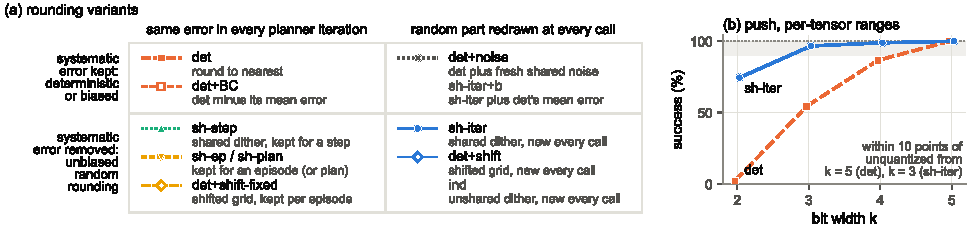
\includegraphics[width=\linewidth]{fig_schematic.pdf}
\caption{(a) Rounding variants (Table~\ref{tab:variants}) by whether they keep the systematic error of round-to-nearest (rows) and whether their error stays the same in every planner iteration or its random part is redrawn at every call (columns). (b) Success on push with per-tensor ranges against bit width $k$ (Section~\ref{sec:bits}; 90 paired episodes per point): within 10 points of the unquantized planner (shaded) from $k^*=\nv{e12.push.pt.kstar.det}$ under \dtm and from $k^*=\nv{e12.push.pt.kstar.shiter}$ under \shiter.}
\label{fig:schematic}
\end{figure}

% =====================================================================================================
% CLAIMS v2: positions C1-C4 against prior and concurrent work (PLAN 4.8, 4.9). No figure or table.
% Concurrent work after our arXiv v1 (2026-11-09), cited as concurrent without dates (double-blind): WM-Quant
%   (2611.21882), Search or Scoring? (2611.25347), LAQ (2611.25614), planner/hardware co-design (2611.22483).
% Their details were checked against the papers on 2026-11-22 (REFERENCES_CHECK.md sec. 3). Goodhart in the Planner
%   (2611.09670) and LoopQ (2611.05093) predate our v1 and are cited as prior work.
\section{Related Work}
\label{sec:related}

\textbf{Quantized world models and policies.} Post-training quantization of DINO-WM makes the planning objective and task success diverge at aggressive bit widths~\citep{fu2026wmquant}, and success depends on which modules keep their precision~\citep{ranganath2026bits}; for quantized world action models, offline action deviation predicts the closed-loop loss~\citep{xu2026prede}. A calibration objective recovers full-precision planning with 4-bit weights~\citep{anon2026modulemse}. Quantized vision-language-action and world action models are calibrated and benchmarked in closed loop~\citep{quantwams2026, vlaquantbench2026, qvla2026, park2026qcrl, loopq2026} and deployed with fused low-bit kernels~\citep{wang2026steerquant, anon2026wamptq, anon2026loopquant}, and quantization error has been reported to recur across their denoising loops~\citep{anon2026loopquant}.

\textbf{Concurrent work.} \citet{wmquant2026} find that quantization error in JEPA-style world models compounds over predictor steps until action rankings become near-random, and their calibration, which includes activation ranges learned per rollout step, brings planning with 4-bit weights and activations (W4A4) close to full precision on some tasks; our rollout-chosen ranges (Section~\ref{sec:bits}) are a simplified form of that range calibration, with one range per layer for all rollout steps. In a quantized world action model, an injected error of equal energy damages the predicted future more when held fixed across the denoising steps than when redrawn at every step~\citep{laq2026}, an analogue of our persistence axis without a planner. The works above calibrate, allocate bits or train; none randomizes rounding at inference or separates how the error is shared from how long it persists.

\textbf{Prediction error versus decisions.} Prediction error averaged over data need not track control performance~\citep{lambert2020mismatch}; decision-relevant error measures track planning quality better~\citep{you2026predictability, wang2026drpe}, and \citet{min2026lowerror} split end-point error across a candidate pool into a pool-common and an action-relative part. Iterating planners have been found to concentrate their candidates in regions where the model cannot rank them~\citep{anon2026elitecert, anon2026resolution}; replacing early CEM rounds with a deterministic approximation hurts while score noise of the same size does not~\citep{anon2026evaluations}, and harder MPPI search against a learned reward model lowers the true return while its held-out accuracy stays high~\citep{goodhart2026planner}. In concurrent diagnostics, rounding a predictor's weights to nearest at low bit widths turns most PushT failures into scoring rather than search failures~\citep{searchscoring2026}. These studies diagnose where a planner fails; we ask which property of the error it exploits, at a fixed per-entry error distribution.

\textbf{Exploitation and rounding rules.} Planners exploit model error~\citep{boney2019dae}, which is essentially unavoidable on large policy sets~\citep{bhamidipaty2026exploitable}; \citet{ha2018worldmodels} injected temperature noise into imagined rollouts so that the controller could not exploit them, and under noisy evaluations CEM optimizes a quantile rather than the mean~\citep{goschin2013cem}. Policy search on fixed random scenarios~\citep{ng2000pegasus} overfits to them, and changing the scenarios as the search proceeds reduces the overfitting~\citep{strens2002paired}. Re-evaluating candidates under redrawn noise is standard in noisy evolution strategies~\citep{hansen2009uncertainty}. Dither decorrelates quantization error from the signal~\citep{roberts1962picture, schuchman1964dither}. Randomized quantization controls limit cycles in recursive digital filters~\citep{kieburtz1977limit} and makes quantized average consensus, which fails under deterministic quantization, converge~\citep{aysal2008consensus}, and unbiased stochastic rounding keeps bias from accumulating~\citep{gupta2015limited, croci2022sr}. Comparisons of rounding rules for low-precision language-model inference give mixed results~\citep{chatelain2026sr, khilar2026dither, wu2026decisions}. These results concern error that accumulates within one computation; we study the selection bias a planner adds when it chooses among candidates across iterations.

% =====================================================================================================
% CLAIMS v2: definitions behind every claim (variants: C2, C4; metrics: all; k* and G: C4; rho_p, sigma_e/sigma_J: C5).
% Table 1 (variants: shared, redrawn, unbiased, error variance). The stage table (tab:setup) is in Appendix C (page budget).
% PLAN 4.6: "no calibration" -> "per-tensor percentile ranges, no error-minimizing calibration"; ranges set on held-out data.
\section{Setup}
\label{sec:setup}

\subsection{Sampling-based planning}
For $I$ iterations per control step, a planner samples $N$ candidate action sequences of horizon $H$ from a Gaussian, predicts the return of each with the world model and refits the Gaussian to the best ones; it then executes the first action of the final plan. CEM refits to the mean and standard deviation of the top $K$ candidates~\citep{rubinstein1999cem}; MPPI weights the top candidates (elites) by $\exp(\beta(J-J_{\max}))$~\citep{williams2017mppi}. Every iteration thus compares candidates through the same quantized network ($N\times I\times H$ calls per control step).

\subsection{Quantization and rounding variants}
\label{sec:variants}
We quantize hidden activations: the four hidden layers of the dynamics and reward MLPs of TD-MPC2 (after Mish) and the six MLP outputs of the DINO-WM predictor (after GELU). Each layer uses a uniform $k$-bit grid on $[\mathrm{lo},\mathrm{hi}]$ with step $\Delta=(\mathrm{hi}-\mathrm{lo})/(2^k-1)$. The default range is per tensor, from the minimum to the 99.99th percentile of held-out activations, with no error-minimizing calibration; Section~\ref{sec:bits} adds per-channel ranges and ranges chosen by rollout error. Inputs, weights and all other modules stay in floating point except in the integer kernels of Section~\ref{sec:cost}. Table~\ref{tab:variants} defines the rounding variants. The dither variants \ind, \shiter, \shstep and \shep use the same kind of unbiased draw and hence the same per-entry error distribution; they differ in how $u$ is shared and how long it is kept. The variants \detshift and \detshiftfix (subtractive dither: round-to-nearest on a randomly shifted grid) share another distribution, with the error variance of \dtm. In open-loop CEM, \shstep and \shep coincide and we call them \shplan. The variant \detbc subtracts a per-unit bias vector $b$, estimated on held-out rollouts by a damped fixed-point iteration until the residual mean error of every layer is below 1\% of $\Delta$ (Appendix~\ref{app:details}); it is the standard bias correction of post-training quantization~\citep{nagel2019dfq} and costs nothing at deployment, since $b$ folds into the next layer's bias.

\begin{table}[t]
\caption{Rounding variants at bit width $k$ ($x$ is the input in grid units, $u\sim U[0,1)$, $o\sim U[-\tfrac12,\tfrac12)$; draws have one entry per unit of a layer, per token and unit in DINO-WM). ``Shared'': one draw serves every candidate. ``Fixed'': the draw (or the rounding error) is the same in every planner iteration. ``Unbiased'': zero mean error over the draw. Error variances assume a uniformly distributed fractional part of $x$; the bias $b$ shifts the mean error, not the variance.}
\label{tab:variants}
\centering\footnotesize
\setlength{\tabcolsep}{3.5pt}
\begin{tabular}{@{}ll>{\raggedright}p{5.0cm}cccc@{}}
\toprule
Variant & Output & Draw & Shared & Fixed & Unbiased & Error variance \\
\midrule
\dtm & $\mathrm{round}(x)$ & none (a fixed function of $x$) & -- & yes & no & $\Delta^2/12$ \\
\detbc & $\mathrm{round}(x)-b$ & none; $b$ per unit, from held-out data & -- & yes & mean removed & $\Delta^2/12$ \\
\ind & $\lfloor x+u\rfloor$ & $u$ per entry and candidate, every call & no & no & yes & $\Delta^2/6$ \\
\shiter & $\lfloor x+u\rfloor$ & $u$ per layer, every call & yes & no & yes & $\Delta^2/6$ \\
\shstep / \shep & $\lfloor x+u\rfloor$ & $u$ per layer and horizon step, once per control step / episode & yes & yes & yes & $\Delta^2/6$ \\
\detshift & $\mathrm{round}(x-o)+o$ & $o$ per layer, every call & yes & no & yes & $\Delta^2/12$ \\
\detshiftfix & $\mathrm{round}(x-o)+o$ & $o$ per layer and horizon step, once per episode & yes & yes & yes & $\Delta^2/12$ \\
\shiterb & $\lfloor x+u\rfloor+b$ & as \shiter; $b$ as \detbc & yes & bias only & no & $\Delta^2/6$ \\
\detnoise & $\mathrm{round}(x)+u-\tfrac12$ & as \shiter & yes & \dtm part & no & $\Delta^2/6$ \\
\bottomrule
\end{tabular}
\end{table}

\subsection{Models, tasks and planners}
TD-MPC2~\citep{hansen2024tdmpc2}: the official 5M single-task checkpoints (three seeds) on 8 Meta-World tasks~\citep{yu2019metaworld}, scored by success, and 4 DMC tasks~\citep{tassa2018dmc}, scored by return, planned with the default MPPI (512 candidates including 24 policy trajectories, 64 elites, 6 iterations, horizon 3); and the official 317M multi-task checkpoint (mt80; prior work distilled and quantized it to FP16, \citealt{kuzmenko2025tdmpcopt}) on the same 8 Meta-World tasks. The Meta-World tasks are push, pick-place, door-open, drawer-open, button-press-topdown, peg-insert-side, window-open and sweep-into, and the DMC tasks cheetah-run, walker-walk, quadruped-walk and finger-turn-hard; we write button-press, peg-insert, cheetah, walker, quadruped and finger. DINO-WM~\citep{zhou2025dinowm}: the official PushT, Wall and PointMaze models with open-loop CEM (300 candidates, top 30, horizon 5, 30 iterations on PushT and 10 otherwise). Per task, a rule picks the primary bit width $k$ on held-out episodes as the largest $k$ at which \dtm loses at least 20 points of success (20\% of return on DMC). The main benchmark tests $k-1$, $k$ and $k+1$: 36 cells (one task at one bit width) for TD-MPC2 at 5M and 9 for DINO-WM. We call push, pick-place, cheetah-run and PushT at their primary bit widths the mechanism tasks. Later experiments use new seed ranges and, for DINO-WM, a new evaluation split, so their cells shared with the main benchmark are replications on independent episodes with the same checkpoints. We describe each experiment where its results appear; the appendices number them E1--E17 (Table~\ref{tab:setup} in Appendix~\ref{app:details}).

\subsection{Metrics and statistics}
\label{sec:stats}
Every variant is paired with the unquantized model on the same episode seeds and planner noise (90 pairs per cell for TD-MPC2: three checkpoints $\times$ 30 seeds, or one 317M checkpoint $\times$ 90 seeds; 100 for DINO-WM). The damage $D$ is the drop from that baseline in percentage points of success (points; \% of return on DMC). A cell is \emph{damaged} if \dtm's drop is significantly greater than zero in a one-sided paired bootstrap test ($10^4$ resamples; $\alpha=0.025$ in the main benchmark and the experiments planned with it, and $0.05$ later), with Holm correction~\citep{holm1979} over the bit widths of a task in the main benchmark and over the cells of a benchmark later. A variant $v$ removes the fraction $\red=(D_{\dtm}-D_v)/D_{\dtm}$ of the damage, \emph{repairs} a cell if $\red\ge0.5$, and is \emph{harmful} if the lower bound of the 95\% interval of $D_v-D_{\dtm}$ exceeds 5 points. Intervals are 95\% paired-bootstrap percentile intervals; the bootstrap resamples pairs, so intervals are conditional on the checkpoints. The smallest usable bit width $k^*$ of a configuration is the smallest $k$ such that $D\le\tau$ ($\tau=10$ points; 10\% on DMC) at $k$ and at every larger tested $k$, and the bits gained by dither are $G=\min(k^*_{\dtm},k^*_{\detbc})-\min(k^*_{\shiter},k^*_{\detshift})$; the DINO-WM sweep has no \detshift arm, so there the second minimum is $k^*_{\shiter}$. Each experiment's hypotheses, thresholds, seeds and analysis code were fixed in a design document before its data existed; analyses and cells added after we had seen results are labeled post hoc (Appendix~\ref{app:plan}).

\subsection{Measuring exploitation}
\label{sec:oei}
Let $e(a)$ be the cost error of candidate $a$: the return that the unquantized model predicts for $a$ minus the return that the quantized model predicts (for DINO-WM, the quantized minus the unquantized planning cost), so that $e(a)<0$ when quantization makes $a$ look better. The optimizer exploitation index $\mathrm{OEI}=e(a_{\mathrm{exec}})-\bar e_{\mathrm{first}}$ compares the executed plan with random first-iteration candidates and splits exactly into a \emph{selection} term (the last iteration's pick against its population) and a \emph{drift} term, the change in the population-mean error from the first to the last iteration. Negative drift means the planner moved its population toward candidates that the error favors; for \dtm we also report the drift share $S=\mathrm{drift}/\mathrm{OEI}$. The cost of persistence, the extra damage from keeping a draw for an episode at an equal per-entry error distribution, is $\dpers=D_{\detshiftfix}-D_{\detshift}$ or, where \detshiftfix was not run, $D_{\shep}-D_{\shiter}$ ($D_{\shplan}-D_{\shiter}$ in DINO-WM). The latent $n$-step error of a variant is its squared error against the unquantized model's $n$-step latent prediction on the first-iteration candidates, relative to the variance of that prediction and averaged over episodes and, for randomized variants, three draws (Appendix~\ref{app:details}). On held-out states common to all variants we also record the persistent share $\rho_p$ (the correlation of $e(a)$ between two evaluations of one candidate set under the random states of consecutive iterations) and the relative spread $\sigma_e/\sigma_J$ (the spread of $e(a)$ across candidates relative to that of the predicted returns).

% =====================================================================================================
% CLAIMS v2: C1 (phenomenon and replication) in 4.1; C5 (offline errors, summary statistic) in 4.2.
% Figure 2 = fig_damage (build/make_figs.py). tab:overview (tables/tab_overview.tex, generated) is in Appendix I.
% PLAN 4.6: "37 of 44" split by measurement condition (5M+DINO-WM 29/36; 317M 8/8); E13 common-state values added.
\section{Deterministic Rounding Breaks Planning}
\label{sec:break}

\subsection{Damage and repair at a glance}
\label{sec:glance}
Round-to-nearest costs up to \nv{e1.maxdet} points (button-press at \nv{e1.maxdet.k} bits). In the main benchmark, \shiter removes at least half of the damage in all \nv{e1.mw.naff} damaged Meta-World cells (a median of \nv{e1.mw.redmed}\%) and in \nv{e1.dw.nfix} of \nv{e1.dw.naff} DINO-WM cells (the exception, PushT at 5 bits, loses only \nv{e1.pusht5.D.det} points under \dtm), and it is not harmful in any of them (Figure~\ref{fig:damage}a). The dither variants share one per-entry error distribution, yet across the damaged Meta-World cells their mean drop ranges from \nv{e1.mw.mean.shiter} points under \shiter to \nv{e1.mw.mean.shep} under \shep, against \nv{e1.mw.mean.det} under \dtm (Table~\ref{tab:overview} in Appendix~\ref{app:new}). On the 317M multi-task model, \shiter removes \nv{e10.red}\% of the damage in all \nv{e10.naff} damaged tasks; the model's primary bit widths (3--5) are close to those at 5M (3--4), so we see no sign that the larger model is more robust to rounding.

\textbf{Replication on new seeds and splits.} The damage reappears on new seeds (Figure~\ref{fig:damage}b): \dtm damages all \nv{e11.td.ndam} TD-MPC2 cells at their primary bit widths, by \nv{e11.mw.ddet} points on Meta-World and \nv{e11.dmc.ddet}\% of return on DMC, and \shiter repairs \nv{e11.b4.n} of the \nv{e11.b4.of} Meta-World cells (all but window-open) without harming any. On new seeds of the 317M model, \dtm damages all \nv{e14.ndam} tasks (\nv{e14.ddet} points), and \shiter repairs all of them. On the new DINO-WM split, \dtm's damage is \nv{dw.wall3.D.det} points on Wall at 3 bits, replicating the exploratory cell of the main benchmark (\nv{e1.wall3.D.det}), and \nv{d4.D.det} points on PushT at 3 bits, a cell we added post hoc, against \nv{d4.e1.D.det} in the main benchmark. PushT at 4 bits did not replicate (\nv{dw.pusht4.D.det} points against \nv{e1.pusht4.D.det}), weak evidence from only \nv{dw.pusht4.nclusters} trajectories; a post hoc re-run of the original pairs on the new GPU type reproduced the original damage, so the split, not the hardware, explains the difference (Appendix~\ref{app:new}). PointMaze at 3 bits has a similar point estimate (\nv{dw.pm3.D.det} against \nv{e1.pm3.D.det}) but is not significant after Holm correction over the three cells. Appendix~\ref{app:new} pools the two splits for PointMaze and Wall but not for PushT.

\begin{figure}[t]
\centering
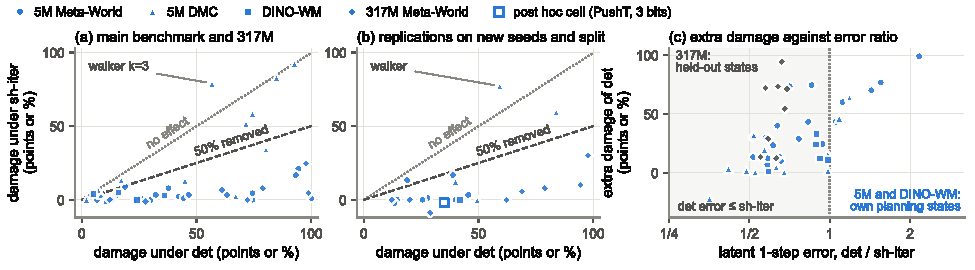
\includegraphics[width=\linewidth]{fig_damage.pdf}
\caption{Damage under \shiter against damage under \dtm (success points on Meta-World and DINO-WM, \% of return on DMC) in every damaged cell of (a) the main benchmark and the 317M model and (b) the replications on new seeds and a new DINO-WM split (Wall at 3 bits; open square: PushT at 3 bits, added post hoc). Below the dashed line \shiter removes at least half of the damage. (c) \dtm's extra damage, $D_{\dtm}-D_{\shiter}$, against the ratio of \dtm's to \shiter's latent one-step error for the cells of (a), on each variant's own planning states in the main benchmark and on held-out states of the unquantized planner at 317M (gray diamonds); in the shaded region \dtm's error is the smaller one.}
\label{fig:damage}
\end{figure}

\subsection{Offline errors and planning damage}
\label{sec:offline}
Although one-step error and damage rank together across bit widths, within a bit width the latent one-step error does not reveal \dtm's damage in most cells. In \nv{e1.h1.n} of the \nv{e1.h1.of} damaged cells of DINO-WM and the 5M TD-MPC2, \dtm's latent one-step error, measured on each variant's own planning states, is no larger than that of \shiter (Figure~\ref{fig:damage}c). Re-measured on held-out states common to all variants, \dtm's error is no larger than \shiter's in \nv{e13.h1common.n} of the \nv{e13.h1common.of} TD-MPC2 cells of the main benchmark, undamaged ones included. At 317M, on held-out states of the unquantized planner, \dtm's latent error is \nv{e10.errratio} times that of \shiter in all \nv{e10.naff} tasks. Errors over more steps distinguish \dtm in more cells: on common held-out states of the TD-MPC2 cells re-run on new seeds, \dtm's error is no larger than \shiter's in \nv{e.e13.err1.n} of \nv{e.e13.ncells} cells over one step, \nv{e.e13.err3.n} over three steps and \nv{e.e13.err5.n} over five steps. In DINO-WM, five-step errors distinguish \dtm too (PushT, 4 bits: \nv{e1.pusht4.err5.det} for \dtm vs.\ \nv{e1.pusht4.err5.shiter} for \shiter). A redefined one-step reward error (Appendix~\ref{app:mech}) is larger for \dtm in \nv{e.e13.rew.n} of \nv{e.e13.ncells} cells.

\textbf{A summary statistic consistent with the mechanism.} On the cells re-run on new seeds and splits, the ranking of the variants' damage within a bit width agrees better with $\rho_p\cdot\sigma_e/\sigma_J$ of the last-iteration candidates than with the latent one-step error: the mean within-cell difference of Spearman correlations is \nv{dg1.mw} on Meta-World (positive in all cells) and \nv{dg1.dmc} on DMC, above the planned threshold of 0.3, but only \nv{dg1.dw} in DINO-WM. Since $\rho_p$ is \nv{e13.rho.fixed} for every fixed variant and \nv{e13.rho.fresh} for every redrawn dither, the statistic nearly restates the manipulated variable, so we report it only as a summary consistent with the mechanism.

% =====================================================================================================
% CLAIMS v2: C2 (two components, double dissociation) in 5.1-5.2; C3 (planner swap) in 5.3; C6 (317M) in 5.1.
% Figure 3 = fig_mechanism; Figure 4 = fig_components, damage removed by each control per family (build/make_figs.py).
% tab:components (tables/tab_components.tex, generated) is in Appendix I. Theory summary 5.4 = E4 (appendix F).
% PLAN 4.6: the general sentence "what decides the outcome is persistence and sharing" is replaced by the two-component
%   statement; no causal "the model decides" (CLAIMS sec. 3).
\section{What the Planner Exploits}
\label{sec:mech}

\subsection{Persistence controls}
\label{sec:persist}
Under \dtm the population-mean error drifts in the favorable direction in all four mechanism tasks at their primary bit widths. We formulated this drift test after the main benchmark, when our original OEI tests had failed (see below). Of that drift, \shiter keeps at most \nv{e2.drift.shiter.max}\% and \detshift at most \nv{e2.drift.detshift.max}\%. Positive controls isolate persistence: holding the \emph{same} shared dither fixed for a control step (\shstep) or an episode (\shep) restores \nv{e2.drift.posctrl}\% of \dtm's drift in the three TD-MPC2 mechanism tasks (Figure~\ref{fig:mech}a). Error size and sharing are equal across these variants; only persistence differs. On PushT the fixed dither with one offset per token and unit did not reproduce the drift (ratio \nv{e2.drift.pusht.shplan}). At 317M, the cost of persistence $D_{\shep}-D_{\shiter}$ has a lower bound above zero in \nv{e14.p2.n} of \nv{e14.ndam} tasks (\nv{e14.p2.range} points; the exception, push, is \nv{e14.push.p2}), and on sweep-into \shep loses \nv{e14.sweep.r} times as many points as \dtm.

In TD-MPC2 the fix needs an iterating planner. With one MPPI iteration \shiter is no better than \dtm; at 12 iterations its damage is \nv{e2.it12.shiter} points or \% while \dtm's stays at \nv{e2.it12.det} and \shstep's at \nv{e2.it12.shstep} (Figure~\ref{fig:mech}b). With the number of elites fixed, \dtm's $|\mathrm{OEI}|$ and its damage grow with the number of candidates in \nv{e2.h2c.n} of 4 tasks, the dose-response expected from the optimizer's curse~\citep{smith2006curse}. A fixed dither drawn from a table of $N_{\mathrm{eff}}$ offsets hurts less as the table grows (\nv{e3.h4a.n} of \nv{e3.h4a.of} tasks, \nv{e3.h4a.exact} of them exactly at the planned Spearman cut-off of $-0.8$), and at 317M the full-size fixed dither is as harmful as \dtm. Sharing matters in TD-MPC2: $D_{\ind}-D_{\shiter}$, the cost of independent draws per candidate, has a lower bound above zero in \nv{e.e3.crn.n} of \nv{e.e3.ntasks} tasks on new seeds, while in DINO-WM no contrast of sharing or persistence had an interval excluding zero (Appendix~\ref{app:mech}).

\textbf{Theory in brief.}\label{sec:theory} A derivation under a Gaussian sampling model with a locally quadratic cost (Appendix~\ref{app:theory}) shows that redrawn unbiased noise produces no expected drift, whereas a persistent error field moves the population to the minimizer of the smoothed model cost, the bias of sample-average approximation~\citep{kleywegt2002saa}. The derivation's selection and drift terms matched \nv{e4.nruns} simulated MPPI and CEM runs. It also predicted, before the main benchmark was analyzed, that the OEI would be negative even under redrawn noise, because the last iteration's pick benefits from the noise it was selected on; this is why our original OEI tests failed (Appendix~\ref{app:neg}).

\begin{figure}[t]
\centering
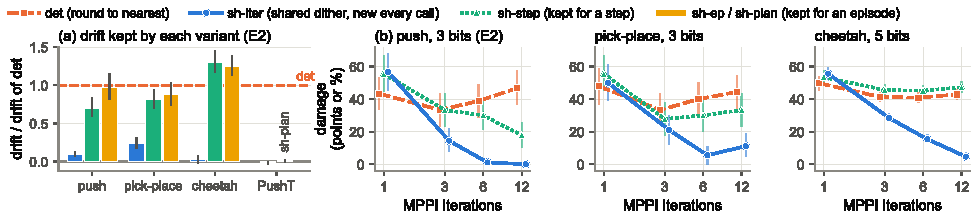
\includegraphics[width=\linewidth]{fig_mechanism.pdf}
\caption{Mechanism sweeps. (a) Favorable drift of the population-mean error kept by each variant, relative to \dtm's own drift (dashed line at 1; TD-MPC2 at its primary bit width; PushT at 4 bits, where \shstep and \shep coincide as \shplan); error bars show 95\% bootstrap intervals. (b) Damage against MPPI iterations (TD-MPC2, 90 paired episodes per point, 95\% intervals).}
\label{fig:mech}
\end{figure}

\subsection{Separating bias, resolution and persistence}
\label{sec:components}
Round-to-nearest error has a per-unit mean, a resolution limit (changes below the grid step vanish) and an input-determined pattern that is the same in every planner iteration. We call the first two together the systematic error. On new seeds and the new DINO-WM split we distinguish the three with the variants of Table~\ref{tab:variants}. If the mean bias causes the damage, \detbc and every unbiased variant repair it, and putting the bias back into redrawn dither (\shiterb) undoes the repair. If the resolution loss causes it, every unbiased randomized rounding repairs it, fixed (\shep, \detshiftfix) or redrawn, and \detbc does not. If the persistent pattern causes it, only the redrawn variants (\shiter, \detshift, \shiterb) repair it. The variant \detnoise keeps \dtm's rounding and adds fresh shared noise; we predicted that it would repair at most half of the damaged cells in every benchmark. Figure~\ref{fig:components} shows the fraction of the damage each variant removes in every damaged cell (counts in Table~\ref{tab:components}).

\textbf{TD-MPC2: persistence dominates.} The cost of persistence $\dpers$ has a lower bound above zero in all \nv{e11.pers.npos} damaged cells (\nv{e11.mw.pers} points on Meta-World, \nv{e11.dmc.pers}\% on DMC). Unbiased random errors held fixed across iterations (\shep, with twice the error variance of \dtm, and \detshiftfix, with the same variance) repair only \nv{e11.mw.nfix.shep} and \nv{e11.mw.nfix.detshiftfix} of the \nv{e11.mw.ndam} Meta-World cells, respectively. Fixed randomized rounding therefore does not repair these cells, which rules out a resolution explanation there. $D_{\shep}-D_{\shiter}$ is positive in all \nv{e11.td.ndam} cells (\nv{e11.shepminusshiter} points or \%), and keeping the draw only within a control step already costs most of this (in the main benchmark, \nv{e1.mw.mean.shstep} points for \shstep against \nv{e1.mw.mean.shep} for \shep and \nv{e1.mw.mean.shiter} for \shiter). The mean bias accounts for part of the damage: \detbc repairs \nv{e11.mw.nfix.detbc} of \nv{e11.mw.ndam} Meta-World cells, \nv{e11.dmc.nfix.detbc} of \nv{e11.dmc.ndam} DMC cells and \nv{e14.nfix.detbc} of \nv{e14.ndam} tasks at 317M. A per-cell classification (persistence \nv{e11.mw.class.persistence}, bias \nv{e11.mw.class.bias} on Meta-World) hinges on cells near the threshold, such as pick-place, where \detbc removes \nv{e11.pickplace.red.detbc} of the damage, so we rely on $\dpers$ and the fixed-versus-redrawn contrast, not on the class counts.

\textbf{DINO-WM: persistence does not dominate.} The new split has two damaged DINO-WM cells, Wall and PushT at 3 bits. Neither cell is dominated by persistence; on PushT we cannot tell whether the mean bias or the resolution loss is at work. In both cells fixed unbiased errors repair the damage (\shplan $\red=\nv{dw.wall3.red.shstep}$ on Wall and \nv{d4.red.shstep} on PushT, \detshiftfix \nv{dw.wall3.red.detshiftfix} and \nv{d4.red.detshiftfix}), as does \shiter (\nv{dw.wall3.red.shiter}, \nv{d4.red.shiter}), and in the main benchmark \shplan repaired PushT at 3 and 4 bits too. Putting \dtm's mean bias back into redrawn dither (\shiterb) or adding fresh noise to \dtm (\detnoise) repairs neither cell ($\red$ \nv{dw.wall3.red.shiterb} and \nv{dw.wall3.red.detnoise} on Wall, \nv{d4.red.shiterb} and \nv{d4.red.detnoise} on PushT). Bias correction (\detbc) repairs Wall ($\red=\nv{dw.wall3.red.detbc.ci}$) but is worse than \dtm on PushT ($\red=\nv{d4.red.detbc}$, and also at 3 bits in the bit sweep and at 4 bits on the new split), so the planned per-cell rule labels Wall bias-dominated and PushT resolution-dominated ($\dpers=\nv{d4.dpers}$ points). Our bias vector $b$, however, does not seem to fit PushT's planning states: subtracting it or adding it (\shiterb) is as harmful as \dtm, and it raises the planning-time latent error (Appendix~\ref{app:baselines}), so \detbc's failure there is not evidence against a mean bias. The DINO-WM evidence rests on two cells, one of them post hoc, and Wall's baseline is unstable: the unquantized model succeeds in \nv{dw.wall3.none}\% of the new pairs against \nv{e1.wall.none}\% of the original ones (\nv{dw.wall.rerun.none}\% when those are re-run on the same machine). Wall's $\dpers=\nv{dw.wall3.dpers}$ points arises because \detshift succeeds \nv{dw.wall3.detshift.better} points more often than the unquantized model. Round-to-nearest at 4 bits also beats the unquantized planner there (by \nv{dw.wall4.det.above} points on the new split and \nv{e1.wall4.det.above} on the original pairs), so the unquantized planner is not an upper bound on Wall and $\red$ can exceed 1.

\textbf{A double dissociation.} Fixed unbiased error and fresh noise thus have opposite effects on Meta-World and DINO-WM, and DMC fits neither pattern: fixed unbiased error repairs both DINO-WM cells but at most \nv{e11.mw.nfix.shep} of \nv{e11.mw.ndam} Meta-World cells, whereas fresh noise added to \dtm repairs all \nv{e11.mw.ndam} Meta-World cells but \nv{d4.comb.detnoise} of the \nv{d4.comb.ndam} DINO-WM cells (Section~\ref{sec:noise}). The three Meta-World cells classified as bias-dominated fall on the persistence side (\detshiftfix removes \nv{e11.mwbias.red.detshiftfix} of their damage, \detnoise \nv{e11.mwbias.red.detnoise}); we leave \detbc out because its effect differs between DINO-WM tasks.

\begin{figure}[t]
\centering
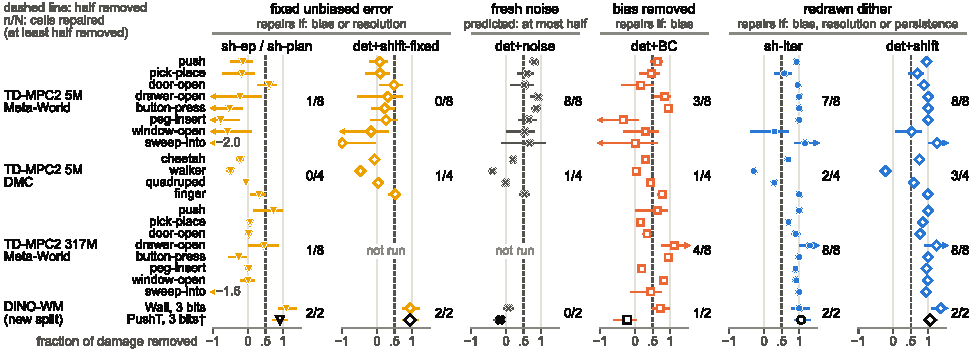
\includegraphics[width=\linewidth]{fig_components.pdf}
\caption{Fraction of the damage removed ($\red$), with 95\% intervals, by each control except \shiterb (Table~\ref{tab:components}) in every damaged cell: TD-MPC2 5M on new seeds (\nv{e11.mw.ndam} Meta-World and \nv{e11.dmc.ndam} DMC cells), the 317M model on new seeds (\nv{e14.ndam} tasks; \detshiftfix and \detnoise not run) and the two damaged DINO-WM cells of the new split (Wall at 3 bits; PushT at 3 bits, post hoc, open black markers); intervals leaving the axis end in an arrowhead. The line above each column names the causes of \dtm's damage that the control would repair (Section~\ref{sec:components}). The dashed line is $\red=0.5$, and $n/N$ counts the cells at or above it.}
\label{fig:components}
\end{figure}

\subsection{Planner swap}
\label{sec:swap}
To test whether the family difference comes from the planners, we swapped their update rules (Table~\ref{tab:e16}). TD-MPC2 with a CEM-like update (uniform elite weights, no policy trajectories, a lower standard-deviation floor) keeps the cost of persistence in all three TD-MPC2 mechanism tasks: $D_{\shep}-D_{\shiter}$ is \nv{e16.td.cem.push}, \nv{e16.td.cem.pickplace} and \nv{e16.td.cem.cheetah} (push, pick-place, cheetah-run), against \nv{e16.td.mppi.push}, \nv{e16.td.mppi.pickplace} and \nv{e16.td.mppi.cheetah} with the default MPPI. Without the policy trajectories \shiter still repairs push and pick-place but not cheetah-run ($\red=\nv{e16.td.cheetah.red.shiter}$). DINO-WM with an MPPI-like update (softmax weights and a standard-deviation floor) shows no cost of persistence that we can distinguish from zero, although \dtm damages PointMaze and Wall under it: $D_{\shplan}-D_{\shiter}$ has upper bounds of \nv{e16.dw.ciupper} points on both tasks with either planner, and the PushT cell at 3 bits gives \nv{d4.shplan.minus.shiter} with CEM. Only the PushT cell at 4 bits, which stayed out of the planned readings because \dtm did not damage it on the new split, gives an interval that excludes zero once its trajectories are resampled (\nv{r5.pusht4.shplan.cluster}). With every swapped planner keeping at least 60\% of the default planner's unquantized success, the pattern followed the model family rather than the update rule. The families differ in whether the interval excludes zero, but cell by cell the sizes overlap: DINO-WM's upper bounds (\nv{r5.dw.ciupper} points, PushT included) exceed TD-MPC2's smallest lower bounds (\nv{r5.td5m.minlower} points on \nv{r5.td5m.minlower.task} at 5M, \nv{r5.td317m.minlower} on push at 317M). The families also differ in architecture, closed versus open loop, horizon and objective, and the swapped planner was not run on PushT, so we do not claim that the model causes the pattern. One hypothesis is table size: DINO-WM's fixed dither has one offset per token and unit, and only coarser tables hurt planning there (Appendix~\ref{app:mech}).

% =====================================================================================================
% CLAIMS v2: C4 (fix, bit limit, noise vs dither, DMC boundary). Figure 5 (new): bit-success curves and k*.
% Figure 6 (new): DMC x iterations and persistent share. FP4 (E9) and QAT/weights stay short (PLAN 4.3: 6.3, 6.4).
% CLAIMS 5.1 item 4: "7/8" is the better of sh-iter and det+shift (sh-iter alone 6/8 PT, 5/8 PC); never pair it with
%   the 2% latency of sh-iter. Item 5: Wall G is 0-2 (borderline). Item 6: det+noise is described by numbers only.
\section{The Fix and Its Limits}
\label{sec:fix}
At the same bit width, \shiter repairs most damaged cells (Section~\ref{sec:glance}). The best post-training quantizer we tested, mostly per-channel ranges, already removes most of \dtm's damage at 3--4 bits (Meta-World $D$ of \nv{e5.pc.mw.range} points), and the extra gain of \shiter on top of it was borderline in TD-MPC2 (\nv{e5.h3b.td} of \nv{e5.h3b.td.of} cells) and found in only \nv{e5.h3b.dw} of \nv{e5.h3b.dw.of} DINO-WM cells. This section sweeps the bit width to ask how far dither lowers the smallest usable bit width $k^*$ on top of better ranges and where the repair stops.\label{sec:bits}

\textbf{Meta-World.} Dither gains at least one bit in \nv{e12.pt.nG} of \nv{e12.mw.n} tasks with per-tensor ranges and in \nv{e12.pc.nG} of \nv{e12.mw.n} with per-channel ranges, counting the better of \shiter and \detshift; \shiter alone gains a bit in \nv{e12.pt.nG.shiter} and \nv{e12.pc.nG.shiter} tasks and \detshift alone in \nv{e12.pt.nG.detshift} and \nv{e12.pc.nG.detshift}. In \nv{e12.mw.n1bit} tasks some rounding rule of the sweep loses at most 10 points at 1 bit, and in all of them that rule is a dither (Figure~\ref{fig:bits}); of the \detnoise curves, added post hoc, only drawer-open per tensor does so (\nv{x5.pt.draweropen1} points), a borderline case whose damage at 2 bits equals the threshold (\nv{x5.pt.draweropen2}). Post hoc, TD-MPC2's FP32 policy without any planning has $D\le\nv{x6.mw.dpol.max7}$ points on 7 of the 8 tasks and $D=\nv{x6.mw.dpol.pickplace}$ points on pick-place (Table~\ref{tab:x6}): the policy alone nearly matches the unquantized planner, so on Meta-World the low-bit results mainly mean that the low-bit planner does not fall below the policy.

\textbf{Robustness of the counts.} In a paired bootstrap over episodes, the task counts stay at or above the planned thresholds in at least \nv{r1.fr.pmin}\% of resamples whichever dither form is counted, and they do so for damage thresholds $\tau$ of \nv{r2.tau} points. Which tasks gain a bit is less stable, in particular pick-place and window-open (Tables~\ref{tab:r1} and~\ref{tab:r2}).

\textbf{DINO-WM and DMC.} On PushT, dither gains \nv{dw.pusht.G} bits with per-tensor ranges and \nv{r1.pusht.pcrc.G} bits with per-channel and rollout-chosen ranges; the bootstrap supports at least one bit with all three ranges but two bits only per tensor (Table~\ref{tab:r1}). Ranges chosen to minimize the multi-step latent error of planner rollouts (Section~\ref{sec:related}) do not change \dtm's $k^*$ (Figure~\ref{fig:bits}), and dither still gains \nv{r1.pusht.pcrc.G} bits on top of them. On Wall the gain is \nv{dw.wall.G.range} bits, borderline because \detbc's damage at 3 bits ($D=\nv{dw.wall3.D.detbc}$ points) lies just above the 10-point threshold. PointMaze gains \nv{dw.pm.G} bits. On DMC the gain is mostly zero (per tensor \nv{e12.dmc.G.pt}; per channel \nv{e12.dmc.G.pc} for cheetah, walker, quadruped and finger), but the policy alone loses \nv{x6.dmc.dpol}\% of return, and the lowest-bit dither planner (per channel, \nv{x6.dmc.k} bits) beats the policy in \nv{x6.dmc.better} of 4 tasks.

\begin{figure}[t]
\centering
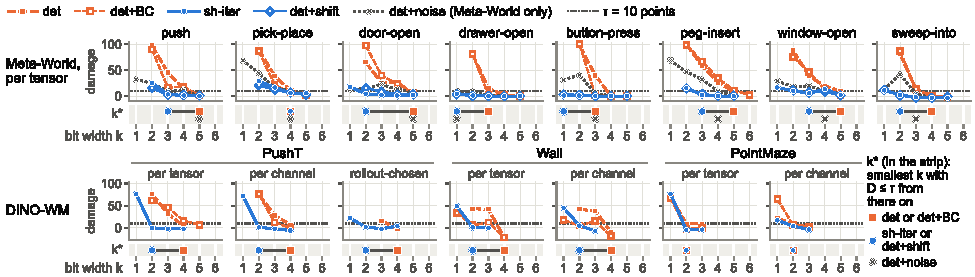
\includegraphics[width=\linewidth]{fig_bitlimit.pdf}
\caption{Damage (success points) against bit width $k$ on Meta-World with per-tensor ranges (per-channel ranges in Figure~\ref{fig:bitspc}) and on DINO-WM with per-tensor, per-channel and, for PushT, rollout-chosen ranges; \detnoise only on Meta-World, post hoc. Dotted line: $\tau=10$ points; missing markers: not run. The strip under each panel marks the smaller $k^*$ of \dtm and \detbc (square; \dtm only with rollout-chosen ranges), of \shiter and \detshift (circle; \shiter only on DINO-WM) and $k^*$ of \detnoise (cross); the gap from square to circle is the point estimate of $G$, which the bootstrap supports less on DINO-WM (Section~\ref{sec:bits}).}
\label{fig:bits}
\end{figure}

\textbf{Fresh noise versus dither.}\label{sec:noise} Contrary to our prediction (Section~\ref{sec:components}), adding fresh shared noise to \dtm (\detnoise) repairs all \nv{e11.mw.ndam} damaged Meta-World cells ($\red$ \nv{e11.mw.red.detnoise}). It repairs \nv{e11.dmc.nfix.detnoise} of \nv{e11.dmc.ndam} DMC cells (finger, the one cell classified as bias-dominated) and \nv{d4.comb.detnoise} of the \nv{d4.comb.ndam} damaged DINO-WM cells ($\red$ \nv{dw.wall3.red.detnoise} on Wall, \nv{d4.red.detnoise} on PushT); dither repairs more in both (\detshift \nv{e11.dmc.nfix.detshift} and \shiter \nv{e11.dmc.nfix.shiter} of the DMC cells; on Wall $\red$ \nv{dw.wall3.red.shiter} for \shiter and \nv{dw.wall3.red.detshift} for \detshift). Its persistent share $\rho_p$ on the last-iteration candidates of the cells re-run on new seeds, \nv{e13.rho.detnoise}, lies between that of the fixed variants (\nv{e13.rho.fixed}) and that of redrawn dither (\shiter \nv{e13.rho.e11.shiter}, \detshift \nv{e13.rho.e11.detshift}); we did not test whether this difference relates to which cells are repaired, nor did we identify why dither repairs more. On the bit axis, \detnoise gains fewer bits than dither. It gains at least one bit over \dtm and \detbc in \nv{x5.pt.nG} of \nv{e12.mw.n} Meta-World tasks per tensor and \nv{x5.pc.nG} per channel, against \nv{e12.pt.nG} and \nv{e12.pc.nG} for dither, and its $k^*$ is no larger than that of \shiter in only \nv{x5.pt.le.shiter} and \nv{x5.pc.le.shiter} tasks. Its damage is also often not monotone in the bit width (per tensor, door-open loses \nv{x5.pt.dooropen3} points at 3 bits but \nv{x5.pt.dooropen2} at 2).

\textbf{Where it helps less: DMC and planner iterations.}\label{sec:dmc} At the default six MPPI iterations, \shiter repairs \nv{e11.dmc.nfix.shiter} of \nv{e11.dmc.ndam} DMC cells on new seeds (and \nv{e1.dmc.nfix} of \nv{e1.dmc.naff} in the main benchmark, where it is harmful on walker at 3 bits: \nv{e1.walker.D.shiter}\% of return lost vs.\ \nv{e1.walker.D.det}\% under \dtm). The drift share $S$ of \dtm is lower on DMC (\nv{e3.share.dmc}) than on Meta-World (\nv{e3.share.mw}), and across the 12 TD-MPC2 tasks it is rank-correlated with the damage that \shiter removes (Spearman \nv{e3.spearman}, new seeds; Figure~\ref{fig:iters}a). With 12 iterations, the better of \shiter and \detshift repairs \nv{e15.it1.n} of the 4 DMC tasks, and its $\red$ grows monotonically from 6 to 12 to 24 iterations in \nv{e15.it2.n} tasks (Figure~\ref{fig:iters}b--e), at the cost of planning time (cheetah-run: \nv{e15.cheetah.detk1.ms}~ms per control step with 6 iterations, \nv{e15.cheetah.ds24.ms}~ms with 24). On \nv{e15.it1.n} of the 4 DMC tasks the fix is thus limited by the number of planner iterations; walker-walk is not repaired at any iteration count we tested ($\red$ \nv{e15.walker.red24} at 24 iterations).

\textbf{Number formats, training and weights.}\label{sec:fp4} Block-scaled FP4 activations reduce the failure in TD-MPC2. With NVFP4~\citep{nvidia2025nvfp4}, \dtm damaged \nv{e9.nvfp4.ndam} of 12 tasks and with MXFP4~\citep{rouhani2023mx} \nv{e9.mxfp4.ndam}; on cheetah-run \dtm lost \nv{e9.nvfp4.cheetah}\% and \nv{e9.mxfp4.cheetah}\% of return, against \nv{e1.cheetah4.D.det}\% with a uniform 4-bit grid; where damage remained, \dtm's latent one-step error was again the smaller one (Appendix~\ref{app:cells}). Our quantization-aware-training baseline was weak and weight quantization exploratory (Appendix~\ref{app:baselines}).

\begin{figure}[t]
\centering
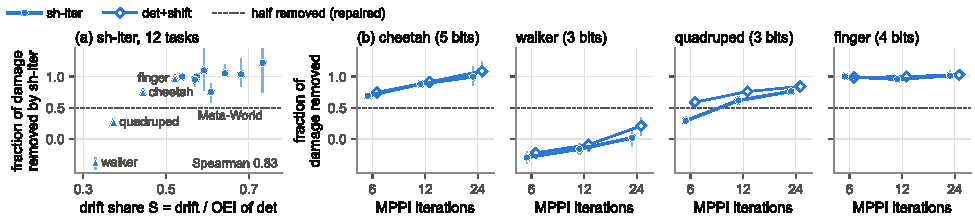
\includegraphics[width=\linewidth]{fig_iterations.pdf}
\caption{(a) Drift share $S=\mathrm{drift}/\mathrm{OEI}$ of \dtm against the fraction of the damage that \shiter removes with the default planner, over the 12 TD-MPC2 tasks (circles Meta-World, triangles DMC; Spearman \nv{e3.spearman}). (b--e) DMC: fraction of the damage removed by \shiter and \detshift against MPPI iterations (90 paired episodes at 6 and 12 iterations, 60 at 24; 95\% intervals).}
\label{fig:iters}
\end{figure}

% =====================================================================================================
% CLAIMS v2: C7 (cost and integer path). Figure 7 = fig_latency (build/make_figs.py). PLAN 4.5: speed is the cost of the fix,
%   not a contribution; A40 pre-converted BF16 is faster and is said so. det+shift is a mechanism control and one form of
%   the fix, not a co-equal prescription (T3, K1 failed). CLAIMS sec. 3: never "W8A4 faster than BF16".
\section{Cost of the Fix}
\label{sec:cost}
\textbf{Overhead and the integer path.} We timed the world-model rollouts of one control step in the fused Triton~\citep{tillet2019triton} kernel of our integer path (int8 weights, 4- or 8-bit activation codes, shared dither drawn on the GPU) as one CUDA graph on an NVIDIA A40 at 5M and 317M parameters and $N\in\{512, 2048, 8192\}$ candidates. In all six conditions, \shiter adds at most \nv{e17.shiter.overhead.max}\% to their latency, because one draw per layer and call serves every candidate (Figure~\ref{fig:latency}c, Appendix~\ref{app:latency}). The variant \detshift adds \nv{e17.detshift.big}\% at $N\ge2048$ but \nv{e17.detshift.5m512}\% (5M) and \nv{e17.detshift.317m512}\% (317M) at $N=512$, because its offset correction reads the next layer's weights once more per call. For this reason we use \detshift as a mechanism control and as one form of the fix, and we recommend \shiter. The integer kernel reproduces the fake-quantization results: $D_{\dtm}-D_{\detshift}$ has the same sign and overlapping intervals in \nv{e17.k2.n} of 4 tasks, including walker, where \detshift is worse than \dtm in both implementations. Per-channel ranges, folded into the next layer's weights because standard integer stacks take activation scales per tensor, match fake quantization in \nv{e17.pc.n} of \nv{e17.pc.of} cells.

\textbf{Latency against floating point.} Replayed as CUDA graphs, the integer rollout with 8-bit weights and 4-bit activations (W8A4) is \nv{e8.speedup}$\times$ faster than FP32 in all 12 conditions of each of two runs on separate A40 instances. BF16 with the weights converted once in advance, however, is the fastest float format in all \nv{e8c.bf16fastest} conditions of the second run, and our integer rollout takes \nv{e8c.int.over.bf16}$\times$ its time (Figure~\ref{fig:latency}a; much of the gap is the first layer, which we keep in FP32, Appendix~\ref{app:latency}). The whole planning step gains less (\nv{e8c.step.speedup}$\times$ over FP32, \nv{e8c.step.over.bf16}$\times$ the time of pre-converted BF16; Figure~\ref{fig:latency}b), since the dynamics and reward networks take only \nv{e8c.wmshare}\% of an FP32 step; shared dither adds at most \nv{e8c.step.overhead.max}\% to it.

Pre-converted BF16 is nearly lossless in closed loop: no damage in \nv{e17.k3.n} of \nv{e17.k3.of} tasks, small damage on door-open (\nv{e17.bf16.dooropen} points) and cheetah-run (\nv{e17.bf16.cheetah}\%), and a small gain on finger. On other hardware low-bit arithmetic can be much faster than 16-bit floating point. An NVFP4 GEMM at the 317M layer width is up to \nv{e8b.nvfp4.gemm}$\times$ faster than BF16 on an RTX 5090, and concurrent work reports custom W4A4 integer kernels that are 1.36--2.13$\times$ faster than PyTorch FP16 on a Jetson AGX Orin~\citep{wmquant2026}.

\begin{figure}[t]
\centering
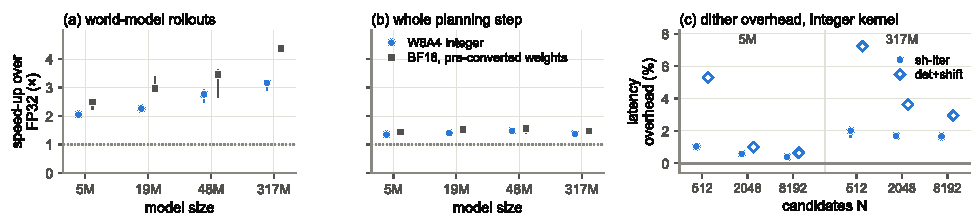
\includegraphics[width=\linewidth]{fig_latency.pdf}
\caption{Latency on an NVIDIA A40 as CUDA graphs (second run): speed-up over FP32 of (a) the world-model rollouts of one MPPI step and (b) the whole planning step, for W8A4 and for BF16 with pre-converted weights (medians over $N$; bars: range); (c) overhead of \shiter and \detshift over \dtm in the fused integer kernel (medians and 95\% intervals over paired blocks).}
\label{fig:latency}
\end{figure}

% =====================================================================================================
% CLAIMS v2: limits of C1-C7 (sec. 2 "한정" items); FINAL_A sec. 6. PLAN 4.6: the RSS "Planned Extensions" list is gone.
\section{Limitations}
\label{sec:limits}
We study two model families, which differ in more than the planner (Section~\ref{sec:swap}), so the family difference is descriptive. The 317M results come from one checkpoint, on Meta-World only, replicated over seeds but on the same GPU type. Each DINO-WM task has one checkpoint, the new split has two damaged cells, one of them post hoc, and the Wall baseline moves between splits. The prescription needs an iterating planner: it does not help with one iteration, needs more than the default iterations on DMC, and on walker-walk at 3 bits is worse than round-to-nearest at the default six. On top of per-channel ranges the bit gain is smaller and absent on PointMaze, and on Meta-World the policy alone nearly matches the unquantized planner; we did not test learned rounding~\citep{nagel2020adaround}, tried outlier-aware scaling~\citep{xiao2023smoothquant, lin2024awq} only in simplified forms (Appendix~\ref{app:baselines}), and did not combine dither with calibration objectives~\citep{anon2026modulemse, wmquant2026}. Our quantization-aware-training baseline was weak, and weights stay in floating point except in the integer kernel. Latency comes from one GPU type and TD-MPC2 only, the FP4 results are fake quantization of the 5M models, and we have no physical-robot experiments. The bit-limit counts rest on a damage threshold; they survive resampling and thresholds of \nv{r2.tau} points, but the per-task results do not.

% =====================================================================================================
\section{Conclusion}
\label{sec:conclusion}
At a fixed bit width and grid, changing only the rounding rule changed whether our low-bit world models planned well. Deterministic rounding error carries a systematic part, which any unbiased randomized rounding removes, and a persistent error field, which an iterating planner exploits and redrawing removes; the second dominates in TD-MPC2 but not in DINO-WM, where a fixed unbiased error repaired both damaged cells. Dither shared by all candidates and redrawn at every iteration removes most of the damage without training and lowers the smallest usable bit width by at least one bit in most Meta-World tasks, even on per-channel grids; since the policy alone nearly matches the unquantized planner there, this means that the low-bit planner does not fall below the policy. The simplest form of this dither adds at most about \nv{e17.shiter.overhead.max0}\% to rollout latency in our integer kernel. Because in most damaged cells the latent one-step error did not distinguish the rounding rules that plan well from those that do not, we recommend validating quantized planners in closed loop.

\section*{Broader Impact Statement}
A low-bit world model can predict well offline and still plan badly, so deploying it on robots without closed-loop validation could cause unsafe behavior. We see no other direct negative societal impact.

% end of the main text (build/build.sh reports where it ends); the references start on a new page, so the last
% page of the main text is not stretched to the full text height
\clearpage
\bibliography{refs}
\bibliographystyle{tmlr}

% =====================================================================================================
\clearpage
\appendix

% PLAN 4.4 A: design document versions (freeze times, SHA-256), what was decided before and after results,
%   deviations (E1-E10: 28 + tolerance fix; E11-E17: D1-D6). Source: FINAL_A 2.4, 8.1; main/LOG.md; tmlr_ext/LOG.md.
\FloatBarrier
\section{Analysis Plan Record}
\label{app:plan}
% Appendix A -- Analysis Plan Record (body; \section and \label stay in main.tex).
% Sources: main/reports/FINAL_A.md 2.4, 2.5, 8.1; main/LOG.md, rss_ext/LOG.md, tmlr_ext/LOG.md (hashes, times);
%   tmlr_ext/DESIGN_tmlr.md sec. 11 (D1-D6). Hashes of v5.1 and of the D5/D6 version: build/make_numbers.py (plan.*).
Each stage's hypotheses, thresholds, seeds, sample sizes and analysis code were frozen in a design document whose SHA-256 hash and time (UTC) were logged before any of the stage's data existed. After freezing, a design document only received additions (rows of its change table and appended sections), so each earlier version can be recovered from the current document; the README of the supplementary material states, version by version, how its logged hash is reproduced. In the supplement, the copies of the main design for v2--v5.3 no longer reproduce their logged hashes because one line naming a server was removed; the copies of the extension, E8c and E11--E17 designs reproduce theirs. The hash of v1 was logged at its freeze, and that of v5.1 only by its first eight hexadecimal digits, in two worker logs. Here a worker is an LLM agent that implemented and ran one group of experiments under the authors' direction, and the coordinator is the LLM agent that assigned work to the workers and kept the main logs; the authors approved every design document and every claim. Operational choices made in short trial runs (smoke tests), such as process counts, block lengths of the latency runs and kernel tile sizes, were recorded before the main runs. Table~\ref{tab:versions} lists the versions and Appendix~\ref{app:tests} the tests they fixed\ifarxiv\else; the hashes are listed in the supplementary material\fi.

\begin{table}[h]
\caption{Versions of the design documents\ifarxiv. Hash = first 12 hexadecimal digits of the SHA-256 of the whole document at that time\fi.}
\label{tab:versions}
\centering\small
\setlength{\tabcolsep}{4pt}
\ifarxiv
\begin{tabular}{@{}>{\raggedright}p{2.6cm}>{\raggedright}p{2.4cm}>{\raggedright}p{2.2cm}>{\raggedright\arraybackslash}p{7.2cm}@{}}
\toprule
Document & Time (UTC) & SHA-256 & What it fixed, and what was known \\
\midrule
Main design v1 & 2026-10-21 18:14 & 9f84ab7f597f & hypotheses, metrics, thresholds and decision rules; TD-MPC2 details; before any E1 data \\
v2 & 2026-10-21 20:01 & 05bf60148145 & DINO-WM details \\
v3 & 2026-10-21 22:54 & 9b86506e744a & DINO-WM OEI reference; PushT evaluation pairs redrawn \\
v4 & 2026-10-22 06:55 & b814a4092a4b & common verdict computation for both families, before the TD-MPC2 E1 results \\
v5, v5.1 & 2026-10-22 09:00, 09:30 & a7895d735cf4, \nv{plan.v51.sha} & E2, E3, E5, E7 details, before their data \\
v5.2 & 2026-10-22 09:50 & 41e1f39d6bd8 & claims narrowed after E1 (OEI diagnostic dropped); H2a$'$, DMC rule \\
v5.3 & 2026-10-24 02:38 & eee46e0aa4f0 & QAT reporting; two post hoc checks \\
Extension design & 2026-10-31 08:46 & c660a10dc72b & E8--E10, before their data \\
E8c design & 2026-10-31 15:51 & 2e9174b32c26 & pre-converted BF16, whole-step graph \\
E11--E17 design v1.0 & 2026-11-21 17:59 & 36d69ea82ef9 & E11--E17, before their data; later D1--D7 appended (its Section 11) \\
E11--E17 design, D5 and D6 & \nv{plan.tmlr.time} & \nv{plan.tmlr.sha} & the post hoc runs X17 and X5 (its Section 11.1), before their data \\
E11--E17 design, D7 & \nv{plan.tmlr.d7.time} & \nv{plan.tmlr.d7.sha} & the post hoc run X6 (its Section 11.1), before its data \\
\bottomrule
\end{tabular}
\else
\begin{tabular}{@{}>{\raggedright}p{3.2cm}>{\raggedright}p{2.6cm}>{\raggedright\arraybackslash}p{9.4cm}@{}}
\toprule
Document & Time (UTC) & What it fixed, and what was known \\
\midrule
Main design v1 & 2026-10-21 18:14 & hypotheses, metrics, thresholds and decision rules; TD-MPC2 details; before any E1 data \\
v2 & 2026-10-21 20:01 & DINO-WM details \\
v3 & 2026-10-21 22:54 & DINO-WM OEI reference; PushT evaluation pairs redrawn \\
v4 & 2026-10-22 06:55 & common verdict computation for both families, before the TD-MPC2 E1 results \\
v5, v5.1 & 2026-10-22 09:00, 09:30 & E2, E3, E5, E7 details, before their data \\
v5.2 & 2026-10-22 09:50 & claims narrowed after E1 (OEI diagnostic dropped); H2a$'$, DMC rule \\
v5.3 & 2026-10-24 02:38 & QAT reporting; two post hoc checks \\
Extension design & 2026-10-31 08:46 & E8--E10, before their data \\
E8c design & 2026-10-31 15:51 & pre-converted BF16, whole-step graph \\
E11--E17 design v1.0 & 2026-11-21 17:59 & E11--E17, before their data; later D1--D7 appended (its Section 11) \\
E11--E17 design, D5 and D6 & \nv{plan.tmlr.time} & the post hoc runs X17 and X5 (its Section 11.1), before their data \\
E11--E17 design, D7 & \nv{plan.tmlr.d7.time} & the post hoc run X6 (its Section 11.1), before its data \\
\bottomrule
\end{tabular}
\fi
\end{table}

\textbf{What was decided after results.} Four groups of rules were fixed after some results of the same study existed, each before the data it governs. After the TD-MPC2 E1 results, v5 and v5.2 fixed the DMC rule, narrowed the mechanism claim from the OEI to drift, and added H2a$'$ and the independently redrawn H2a; these were tested on the new seeds of E2 and E3 and, for PushT, on the 4-bit cell of E1, whose drift had not been computed when the rule was fixed (marked $^\dagger$ in Table~\ref{tab:tests}). After the TD-MPC2 E5 and E7 results, v5.3 fixed how the QAT baseline is reported and added two descriptive checks (QAT without quantization; a paired re-measurement of latency). After E8--E10, the E8c design added pre-converted BF16 and the whole-step graph. Within E11--E17, D3 was decided after the unquantized Wall results on the new split, D4--D6 after the E11 readings, and D7 after a review of the manuscript; the cells they added are labeled post hoc throughout. Analyses chosen after seeing the data they analyze are labeled post hoc.

\textbf{Deviations in E1--E7.} The following deviations from the main design were recorded during the main study. None of them changed a verdict; the tolerance fix described after the list did.
\begin{enumerate}\setlength{\itemsep}{0pt}\setlength{\parskip}{0pt}
\item The rule's ``20 held-out episodes'' was read as the sum over the three checkpoints, which is the E1 condition and gives more episodes (before any E1 data).
\item For tasks whose primary bit width is 3, the cell at 2 bits was included as the rule requires, although 2 lies outside the design's candidate range.
\item No tested bit width gave the 20-point drop on drawer-open or PointMaze, so the pilot's fallback rule (the smallest tested width) was used. On sweep-into, the drop at 3 bits lay exactly at the threshold.
\item Wall: the rule, read literally, chose 5 bits, where the held-out drop lay exactly at the threshold; on the evaluation pairs no Wall cell was damaged, so Wall contributes no tested cell, and the 3-bit cell was added as exploratory.
\item Open-loop CEM makes \shstep and \shep identical, so DINO-WM ran one of them (\shplan).
\item The PushT evaluation pairs were redrawn so that no frame overlaps the held-out frames (v3, before the PushT E1 runs).
\item The DINO-WM OEI was defined against the cost of the unquantized model, correcting the design's ``true cost'' wording (v3, before the OEI analysis).
\item The variant \detshift was defined operationally as one offset per unit, shared by all candidates and redrawn at every forward call.
\item The two families' OEI code differed: TD-MPC2 scored the executed plan with the draw that selected it, DINO-WM with an independent draw. From E2 on both versions were recorded, and the three TD-MPC2 H2a cells were re-measured with independent draws as a post hoc correction; the frozen verdict stands.
\item The H2c sweep was corrected to a fixed number of elites, which the design's extreme-value argument requires (v5.1, before the E2 data); the fixed-ratio sweep ran as an auxiliary for TD-MPC2 only.
\item The clipping grid of the MSE baseline of E5 was widened before the E5 results, because at 3 bits most selected values lay at its lower end; this keeps the baseline from being weak.
\item An auxiliary measure, the variance of the fixed-table error across candidates, was added to E3 (v5.1).
\item The sixth E3 slot of TD-MPC2 was filled with an independent table kept for the episode; walker, where dither had been harmful in E1, was added to the table-size sweep, a choice made after E1 and stated in v5.
\item All settings ran with the protocol's episode counts, which exceeded the design's compute estimate for E2 (cost only).
\item E7: no torchao baseline and no CUDA graphs; success was measured with 4-bit codes held in int8 containers, and packed int4 was used for latency only.
\item The E7 worker saw latency summaries before finishing the code review (disclosed); code changes followed the design text only.
\item Bootstrap Spearman values with ties use average ranks, and the final E3 analysis was run exactly once (before results).
\item H3b, which the design had placed in no family of tests for multiplicity correction, was judged per cell with uncorrected 95\% intervals, as its rule states.
\item DINO-WM H4a eligibility: Wall at 5 bits was excluded because its E1 drop was not significant, and ``majority'' was read as more than half; the other reading gives the same verdict.
\item The weak-baseline caveat attached to the TD-MPC2 QAT (v5.3) was not attached to the DINO-WM QAT, whose result does not show the same signs.
\item The DINO-WM QAT stopped at its time budget, as the design allows.
\item Run order: a second DINO-WM chain used the TD-MPC2 GPU once it was free, and the QAT stages moved to the other GPU (allowed by v5).
\item E2 DINO-WM: the same-draw selection term of \shiter needs a second GPU pass and was reported in its elite form.
\item The E1 DINO-WM worker deleted its own test files outside its working directory, against the run rules (no data affected).
\item The theory worker briefly exceeded its CPU-process limit (no data affected).
\item The optional E6 (other deterministic error sources: activation sparsification, and an offline test on a larger world model) was not run, so H6 has no evidence.
\item Two post hoc checks (QAT without quantization; paired latency re-measurement) were added in v5.3 as descriptive results.
\item Routine monitoring was paused twice, which delayed the detection of one stalled run queue; no result changed.
\end{enumerate}

\textbf{Tolerance of threshold comparisons.} SciPy returns Spearman correlations whose exact value is $\pm0.8$ as $\pm0.7999999999999999$. Before any H2c or H4a result was computed, every threshold comparison of both families was changed to use a tolerance of $10^{-9}$, and later stages kept it. The fix decides H4a: without it, H4a would fail in both families, because \nv{e3.h4a.exact} of the \nv{e3.h4a.n} passing tasks sit exactly at $-0.8$.

\textbf{E8--E10 and E8c.} These ran as designed. Implementation choices that the design delegated to the workers were made by timing \dtm only, as prescribed, and recorded before the main measurements; the E10 bit width of sweep-into was chosen at a held-out drop exactly at the threshold, under the tolerance rule. The comparison with pre-converted BF16 of an integer rollout whose first layer runs in TF32 was chosen after the E8c results and is labeled post hoc.

\textbf{Deviations in E11--E17.} The E11--E17 design records seven changes after its freeze (Section 11 of the E11--E17 design document). D1 and D2 were decided before any data they affect; D3--D7 were decided after some results and are labeled post hoc. D1--D3 were decided by an LLM agent under a procedure the authors had set in advance for the unattended runs: questions that would change the design went to a separate LLM agent, which decided from information available before the affected results, and claims could change only with the authors' approval. D4--D7 were decided by the authors, D5--D7 on the proposal of LLM agents.
\begin{enumerate}\setlength{\itemsep}{0pt}\setlength{\parskip}{0pt}
\item[D1.] PushT split: the design required new evaluation pairs sharing no frame with any earlier split, but earlier splits had used almost every frame of the validation trajectories. Pairs were drawn excluding all frames of the held-out split, the trial-run (smoke) split and the E1 split, and sharing as few frames as possible with the split used in E0 to reproduce the published DINO-WM results; the new pairs come from \nv{dw.pusht4.nclusters} trajectories, so a bootstrap over trajectories is reported alongside (before any planning on the new split).
\item[D2.] Bias vector: the design's three undamped sweeps $b\leftarrow b+m$ failed the convergence check in all three model groups (diverging or oscillating in TD-MPC2, converging too slowly in DINO-WM). The rule became $b\leftarrow b+\eta m$ from $b=0$ until the per-unit mean residual of every layer is below 1\% of $\Delta$, with at most 60 updates, trying $\eta=1$, then $\tfrac12$, then $\tfrac14$; a cell that never converges would use the smallest-residual $b$ and be reported both ways (no cell needed this; Appendix~\ref{app:details}). This rule was fixed before any \detbc result with a converged $b$, and episodes run with an old $b$ were discarded.
\item[D3.] Wall baseline: the unquantized model succeeded in \nv{dw.wall3.none}\% of the new Wall pairs, outside the planned window of $\pm10$ points around E1's \nv{e1.wall.none}\%. Re-running the E1 pairs on the same machine gave \nv{dw.wall.rerun.none}\%, so the pipeline was not at fault; the new split was kept and all three baselines are reported (post hoc, before any quantized Wall result).
\item[D4.] PushT at 3 bits was added on the new split after the new split had shown a single damaged DINO-WM cell (post hoc). The planned readings B2, B3 and Dg1 were left unchanged; the cell and the combined DINO-WM reading are reported separately.
\item[D5.] X17: PushT at 4 bits re-run on the E1 pairs on the GPU type of the new split, with a reading rule (i)--(iii) fixed before its data (post hoc).
\item[D6.] X5: the bit curve of \detnoise on Meta-World, per tensor at 1--5 bits and per channel at 1--3 bits, descriptive, fixed before its data (post hoc).
\item[D7.] X6: TD-MPC2's policy without planning (FP32, mean action, no world-model calls) on the 12 tasks of E11, paired with the unquantized planner on the same 90 episodes, descriptive, fixed before its data (post hoc).
\end{enumerate}
Run incidents (out-of-memory failures, a stalled GPU-sharing daemon, an unreachable cloud API) are listed in the coordinator and worker logs; none lost or changed data, and the affected jobs were re-run.


% PLAN 4.4 B: every planned test with its outcome (holds / fails / borderline). Source: FINAL_A 3, CLAIMS_rss, RESULTS_tmlr 0.
\FloatBarrier
\section{All Planned Tests}
\label{app:tests}
% Appendix B -- All Planned Tests (body). Table rows: tables/tabB_tests_e1e10.tex, tabB_tests_e11e17.tex
%   (build/make_tables.py; values from the numbers.tex keys b.*, e1.*, e9.*, e10.*, e11.* ..., computed from the result
%   files). Labels H1, B1, ... appear only in the appendices (PLAN 4.2).
Tables~\ref{tab:tests} and~\ref{tab:tests2} list every planned test with its outcome. Threshold conditions are judged on point estimates, with a tolerance of $10^{-9}$ (Appendix~\ref{app:plan}); a drop counts when it is significantly greater than zero under the test and Holm correction of Section~\ref{sec:stats}, and intervals are 95\% paired-bootstrap intervals. The tests of E1--E7 were fixed in the main design, those of E8--E10 in the extension design, L2c and S1--S3 in the E8c design, and B1--K3 in the E11--E17 design, each before the data of its stage. Rows marked $^\dagger$ were added after the first results and tested on data collected afterwards (for PushT, on E1 episodes not yet analyzed for that quantity); ``borderline'' marks an outcome decided by one cell, one rank or a value exactly at a threshold. The four mechanism tasks are push, pick-place, cheetah-run and PushT at their primary bit widths. Results that no planned test covers, such as the post hoc cells of D4--D6, are reported as descriptive findings in the main text and Appendix~\ref{app:new}.

\begin{table}[t]
\caption{Planned tests of E1--E10 and their outcomes. A benchmark is TD-MPC2 Meta-World, TD-MPC2 DMC or DINO-WM. OEI and drift are defined in Section~\ref{sec:oei}; percentages of DMC are of return. $^\dagger$ added after the first results.}
\label{tab:tests}
\centering\scriptsize
\setlength{\tabcolsep}{3pt}
\begin{tabular}{@{}l>{\raggedright}p{6.3cm}>{\raggedright\arraybackslash}p{7.6cm}@{}}
\toprule
Test & Hypothesis & Outcome \\
\midrule
\inputrows{tables/tabB_tests_e1e10.tex}
\bottomrule
\end{tabular}
\end{table}

\begin{table}[t]
\caption{Planned tests of E11--E17 and their outcomes. $k^*$ and $G$ are defined in Section~\ref{sec:stats}, $\rho_p$ and $\sigma_e/\sigma_J$ in Section~\ref{sec:oei}; percentages of DMC are of return.}
\label{tab:tests2}
\centering\scriptsize
\setlength{\tabcolsep}{3pt}
\begin{tabular}{@{}l>{\raggedright}p{6.3cm}>{\raggedright\arraybackslash}p{7.6cm}@{}}
\toprule
Test & Hypothesis & Outcome \\
\midrule
\inputrows{tables/tabB_tests_e11e17.tex}
\bottomrule
\end{tabular}
\end{table}


% PLAN 4.4 C: checkpoints, quantization sites and ranges, planner settings, seed splits, hardware. Source: DESIGN_main,
%   DESIGN_ext, DESIGN_tmlr 0.2-0.6.
\FloatBarrier
\section{Experimental Details}
\label{app:details}
% Appendix C -- Experimental Details (body). Sources: main/DESIGN_main.md (0, 4, 7), rss_ext/DESIGN_ext.md (0-3),
%   tmlr_ext/DESIGN_tmlr.md (0.2-0.6, 1-7, 11); bias-vector counts: td_summary.json, e14_bias.csv, calib_summary_dw.json.
Table~\ref{tab:setup} lists the stages of the study, which the main text calls experiments, and their cells.

\begin{table}[h]
\caption{Stages, models and cells. Seeds of each stage are disjoint from all earlier ones; the seeds, planners and GPUs of each stage are given below. The optional E6 was not run (Appendix~\ref{app:plan}).}
\label{tab:setup}
\centering\small
\setlength{\tabcolsep}{4pt}
\begin{tabular}{@{}l>{\raggedright}p{4.5cm}>{\raggedright\arraybackslash}p{9.6cm}@{}}
\toprule
Stage & Question & Models and cells \\
\midrule
E1 & damage, repair, offline errors & TD-MPC2 5M: 12 tasks $\times$ 3 bit widths, 7 variants, 90 pairs; DINO-WM: 9 cells (+1 exploratory), 6 variants, 100 pairs \\
E2, E3 & iterations, candidates, table size, sharing vs.\ persistence & TD-MPC2 mechanism tasks (push, pick-place, cheetah-run) and 12 tasks; DINO-WM PushT \\
E4 & derivation against simulation & simulated MPPI and CEM planners on a locally quadratic cost, \nv{e4.nruns} runs on CPUs (Appendix~\ref{app:theory}) \\
E5, E7--E10 & strong post-training baselines, integer kernels, latency, FP4, 317M & TD-MPC2 5M and 317M; DINO-WM \\
E11 & bias vs.\ resolution vs.\ persistence & TD-MPC2 5M: 12 tasks at the primary $k$, 8 variants, 90 pairs; DINO-WM: PushT 4-bit, PointMaze 3-bit, Wall 3-bit, new split, 100 pairs \\
E12 & smallest usable bit width & TD-MPC2 5M 12 tasks and DINO-WM 3 tasks; per-tensor, per-channel and (PushT) rollout-chosen ranges \\
E13 & offline errors on common held-out states & all E1 and E11 cells \\
E14 & persistence at 317M & 8 Meta-World tasks, primary $k$, 6 variants, 90 pairs \\
E15, E16 & DMC $\times$ iterations; planner swap & DMC 4 tasks $\times$ \{6, 12, 24\} iterations; CEM-like TD-MPC2, MPPI-like DINO-WM \\
E17 & integer kernel, pre-converted BF16 & TD-MPC2 5M, 4 tasks (kernel) and 12 tasks (BF16) \\
\bottomrule
\end{tabular}
\end{table}

\textbf{Models and code.} TD-MPC2: the official single-task 5M checkpoints of seeds 1, 2 and 3 for the 12 tasks, and the official multi-task checkpoint mt80 of 317M parameters. The official code does not evaluate a multi-task checkpoint on one task, so a wrapper reproduces the training-time observation padding, action mask and task embedding; it matched the official multi-task path bit for bit. DINO-WM: the official PushT, Wall and PointMaze models with their DINOv2 ViT-S/14 encoder~\citep{oquab2024dinov2}. Upstream code is pinned to TD-MPC2 commit \texttt{332f19e}, DINO-WM commit \texttt{0a9492f}, Meta-World \texttt{04be337} and D4RL~\citep{fu2020d4rl} \texttt{89141a6} (for PointMaze), with PyTorch 2.7.1 (CUDA 12.6) for TD-MPC2 and 2.4.1 (CUDA 12.4) for DINO-WM; the FP4 GEMM timings of E8b used the PyTorch of a CUDA 12.8 image. Checkpoint and data files were checked against recorded SHA-256 hashes whenever they were copied to a new machine.

\textbf{Quantization sites and grid.} TD-MPC2 quantizes the Mish outputs of the two hidden layers of the dynamics MLP and the two of the reward MLP; the encoder, the Q-ensemble and the policy stay in FP32. DINO-WM quantizes the six GELU outputs of the predictor's MLP blocks; the encoder and all other modules stay in floating point. With range $[\mathrm{lo},\mathrm{hi}]$, $n=2^k-1$ and $\Delta=(\mathrm{hi}-\mathrm{lo})/n$, an activation $a$ maps to $x=(\mathrm{clip}(a,\mathrm{lo},\mathrm{hi})-\mathrm{lo})/\Delta$ and back to $\mathrm{lo}+\Delta\cdot\mathrm{clamp}(r(x),0,n)$, where $r$ is the rounding rule of Table~\ref{tab:variants}; the offset variants add $\Delta o$ back after clamping, and the bias vector $b$ is subtracted or added after the map. Random draws come from per-episode CUDA generators, so the planner's own random stream is identical across variants; this was checked before the E11--E17 runs and, at 317M, by comparing the planner's random state at the end of every episode across variants.

\textbf{Ranges.} Per-tensor ranges are $[\min, \text{99.99th percentile}]$ of each layer's activations on held-out calibration episodes of the unquantized planner (E0 for the 5M models and DINO-WM, held-out episodes of E10 for 317M); every stage reuses these ranges. Per-channel ranges take the same statistics per unit, recomputed on the cloud machines from held-out data: five calibration episodes (12{,}000 planning inputs, three horizon steps) for TD-MPC2 and 256 calibration windows for DINO-WM. Rollout-chosen ranges (PushT, E12) choose each layer's upper bound from the percentiles $\{99, 99.9, 99.99, 99.999, \max\}$ by two rounds of coordinate descent, minimizing the five-step latent relative error of \dtm on the held-out pairs; this is a simplified form of the range calibration of concurrent work~\citep{wmquant2026}, with one range per layer for all rollout steps and without its other components.

\textbf{Bias vector.} The variants \detbc and \shiterb use one vector $b$ per (task, checkpoint, range, bit width). Starting from $b=0$, the quantized and the unquantized model roll out the same start states and action sequences on held-out data (three steps for TD-MPC2, five for DINO-WM), and $b$ moves by $\eta$ times the per-unit mean of (quantized $-$ unquantized) output of each layer, which also corrects the mean shift that earlier layers and steps produce. The iteration stops when the mean residual of every layer is below 1\% of $\Delta$, with at most 60 updates and $\eta=1$, then $\tfrac12$, then $\tfrac14$, each from $b=0$ (deviation D2). All \nv{c.bias.td.n} TD-MPC2 vectors converged (\nv{c.bias.td.a1} with $\eta=1$, \nv{c.bias.td.a2} with $\tfrac12$, \nv{c.bias.td.a4} with $\tfrac14$; at most \nv{c.bias.td.maxupd} updates), as did the eight 317M vectors (\nv{c.bias.mt.a2} with $\tfrac12$, \nv{c.bias.mt.a4} with $\tfrac14$; at most \nv{c.bias.mt.maxupd} updates, from ten held-out episodes per task) and the \nv{c.bias.dw.n} DINO-WM vectors (all with $\eta=1$; at most \nv{c.bias.dw.maxupd} updates). Because no vector failed to converge, the two readings that D2 prescribes for that case coincide. Appendix~\ref{app:baselines} reports how well $b$ fits outside its data.

\textbf{Latent errors.} The planning-time errors of E1 are measured on the first-iteration candidates of up to eight planning states per TD-MPC2 episode and of every DINO-WM episode, against the unquantized model on the same candidates; randomized variants average three dither draws, and a cell averages its episodes. For TD-MPC2, the $n$-step error is $\sum_i\|z^{q}_{i,n}-z^{0}_{i,n}\|^2$ over the candidates $i$, divided by their number and by the variance of the unquantized latents $z^{0}_{i,n}$ across them, where $z_{i,n}$ is the open-loop latent prediction after $n$ steps; the one-step error instead feeds the unquantized latent of every horizon position to one quantized step and averages the squared error over the positions, normalized by the variance of all unquantized next latents. For DINO-WM, the error at horizon step $n$ of the first-iteration rollout is the planning cost's distance between the quantized and the unquantized prediction of the same candidate (visual MSE plus $\alpha$ times the proprioceptive MSE), averaged over the candidates and divided by the variance of the unquantized predictions across the candidates. E9 and E10 measure the TD-MPC2 errors on held-out states of the unquantized planner, and E13 on states common to all variants.

\textbf{Planners.} Table~\ref{tab:planners} gives the planner settings. The CEM-like TD-MPC2 planner of E16 sets the MPPI temperature to 0, which weights every elite equally, lowers the standard-deviation floor and drops the policy trajectories. The MPPI-like DINO-WM planner replaces the top-30 mean by a softmax-weighted mean and standard deviation, $w\propto\exp(-J/\lambda)$, with a floor of 5\% of the initial standard deviation; $\lambda$ is $c$ times the standard deviation of the first iteration's elite costs, with $c\in\{0.25, 0.5, 1, 2\}$ chosen by unquantized success on the 20 held-out pairs ($c=\nv{c.e16.c.pm}$ on PointMaze, $\nv{c.e16.c.wall}$ on Wall). Every swapped planner kept at least 60\% of the default planner's unquantized success.

\begin{table}[h]
\caption{Planner settings. MPPI weights the elites by $\exp(\beta(J-J_{\max}))$; CEM refits to the top $K$ candidates. $N$ counts all candidates.}
\label{tab:planners}
\centering\footnotesize
\setlength{\tabcolsep}{3.5pt}
\begin{tabular}{@{}l>{\raggedright}p{2.4cm}cccc>{\raggedright\arraybackslash}p{4.2cm}@{}}
\toprule
Model & Planner & $N$ & Elites & Iterations & Horizon & Other \\
\midrule
TD-MPC2 (default) & MPPI, warm start & 512 & 64 & 6 & 3 & 24 policy trajectories; $\beta=0.5$; std in $[0.05, 2]$ \\
TD-MPC2, E2 & MPPI & 64--1024 & 64 & 1--12 & 3 & elite count, temperature and warm start also varied \\
TD-MPC2, E15 & MPPI & 512 & 64 & 6, 12, 24 & 3 & default otherwise \\
TD-MPC2, E16 & CEM-like & 512 & 64 & 6 & 3 & $\beta=0$; std floor 0.01; no policy trajectories \\
DINO-WM (default) & open-loop CEM & 300 & 30 & 30 (PushT), 10 & 5 & first sample at the mean \\
DINO-WM, E2 & open-loop CEM & 64--1024 & 6--75 & 5--30 & 5 & PushT at 4 bits \\
DINO-WM, E16 & MPPI-like & 300 & -- & 10 & 5 & softmax weights; std floor 5\% \\
\bottomrule
\end{tabular}
\end{table}

\textbf{Seeds and splits.} Every TD-MPC2 cell pairs three checkpoints with 30 episode seeds (one 317M checkpoint with 90 seeds), and the seed range of each stage is new: E0 held-out runs 12000--12019, E1 20000--20029, E2 40000--40029, E3 50000--50029, E5 60000--60029 (QAT data 65000--65019), E7 70000--70029, E9 80000--80029, E10 90000--90089, E11, E12, E15, E16 and X5 100000--100029, E14 102000--102089. Offline errors use held-out states from separate seeds (E9 81000--81029, E10 91000--91029, E13 101000--101029; the 317M bias vectors 103000--103009). DINO-WM pairs a start--goal pair with a planner seed: E1 used 100 evaluation pairs per task (PushT pairs redrawn so that no frame overlaps the 20 held-out pairs), and E11--E16 a new split of 100 pairs with new planner seeds and dither salt (deviation D1 for PushT). DMC cells of E12 and PushT cells start with 45 pairs or 50 episodes and add the rest when the interval contains the threshold; their intervals are not corrected for this interim look.

\textbf{Hardware.} E1--E7 ran on two RTX A5000 GPUs of a local server: TD-MPC2 on one GPU with 16 processes under NVIDIA's Multi-Process Service (MPS), which does not change any episode, and each DINO-WM cell on a single GPU. Later stages ran on rented cloud GPUs: A40 for E8, E8c, E9, E17 and the TD-MPC2 parts of E11--E16 and X5; RTX 5090 for E8b; RTX 4090 for E10, E14, the DINO-WM parts of E11--E16, D4 and X17 (RTX A5000 was unavailable). A variant and its unquantized baseline always ran on the same machine, because the same seeds give bit-identical episodes only on one device and software stack.


% PLAN 4.4 D: per-cell tables of E1 (TD-MPC2 36 cells x 7 variants), DINO-WM, 317M (E10), FP4 (E9, 24 cells).
\FloatBarrier
\section{Per-Cell Results of the Main Stages}
\label{app:cells}
% Appendix D -- Per-Cell Results of the Main Stages (body). Tables: tables/tabD_e1_td.tex, tabD_e1_dw.tex, tabD_e10.tex,
%   tabD_e9.tex (build/make_tables.py from e1_tdmpc2_cells.csv, e1_dinowm_cells.csv, e10_eval.csv, e9_cells.csv).
Tables~\ref{tab:e1td}--\ref{tab:e9} give every cell of E1, E10 and E9. $D$ is the drop from the unquantized model on the same pairs, in success points (Meta-World, DINO-WM) or \% of return (DMC); a cell is damaged ($^\ast$) when \dtm's drop is significantly greater than zero (Section~\ref{sec:stats}; Holm correction over the bit widths of a task, and over the tasks of E10 and of each format in E9). In E1 the latent one-step error is measured on each variant's own planning states, as in Section~\ref{sec:offline}, and in E9 and E10 on held-out states of the unquantized planner. Appendix~\ref{app:new} repeats the E1 measurement on common held-out states. In E1 the dither variants share one per-entry error distribution at each bit width, yet their damage ranges from \shep, often worse than \dtm, through \shstep and \ind to \shiter, which, like \detshift, stays near the unquantized model in most Meta-World cells.

\begin{table}[t]
\caption{E1, TD-MPC2 5M: damage $D$ of every variant (90 pairs) and the latent one-step error of \dtm and \shiter. none = unquantized success (\%) or return; $^\ast$ damaged cell.}
\label{tab:e1td}
\centering\scriptsize
\setlength{\tabcolsep}{3.5pt}
\begin{tabular}{@{}lrrlrrrrrrr@{}}
\toprule
 & & & \multicolumn{6}{c}{$D$} & \multicolumn{2}{c}{latent error} \\
\cmidrule(lr){4-9}\cmidrule(l){10-11}
Task & $k$ & none & \dtm & \ind & \shiter & \shstep & \shep & \detshift & \dtm & \shiter \\
\midrule
\inputrows{tables/tabD_e1_td.tex}
\bottomrule
\end{tabular}
\end{table}

\begin{table}[h]
\caption{E1, DINO-WM: damage of every variant (100 pairs) and the latent one- and five-step errors of \dtm / \shiter. In open-loop CEM \shstep and \shep coincide (\shplan). $^\ast$ damaged cell; $^\circ$ exploratory cell, not part of the tests.}
\label{tab:e1dw}
\centering\scriptsize
\setlength{\tabcolsep}{3.5pt}
\begin{tabular}{@{}lrrlrrrrcc@{}}
\toprule
 & & & \multicolumn{5}{c}{$D$ (points)} & \multicolumn{2}{c}{latent error, \dtm / \shiter} \\
\cmidrule(lr){4-8}\cmidrule(l){9-10}
Task & $k$ & none & \dtm & \ind & \shiter & \shplan & \detshift & 1 step & 5 steps \\
\midrule
\inputrows{tables/tabD_e1_dw.tex}
\bottomrule
\end{tabular}
\end{table}

\begin{table}[h]
\caption{E10, TD-MPC2 317M (one checkpoint, 90 seeds): damage of \dtm and \shiter (points), $\red$ of \shiter, and the latent one-step errors on held-out states of the unquantized planner. Every task is damaged.}
\label{tab:e10}
\centering\scriptsize
\setlength{\tabcolsep}{3.5pt}
\begin{tabular}{@{}lrrlllrr@{}}
\toprule
 & & & & & & \multicolumn{2}{c}{latent error} \\
\cmidrule(l){7-8}
Task & $k$ & none & $D_{\dtm}$ & $D_{\shiter}$ & $\red$ \shiter & \dtm & \shiter \\
\midrule
\inputrows{tables/tabD_e10.tex}
\bottomrule
\end{tabular}
\end{table}

\textbf{FP4 formats (E9).} We repeated the 5M experiment with activations in NVFP4~\citep{nvidia2025nvfp4} (blocks of 16, E4M3 scale) and MXFP4~\citep{rouhani2023mx} (blocks of 32, power-of-two scale), rounding each block to the E2M1 grid to nearest (\dtm) or stochastically (\shiter); weights stay in FP32 and the block scales are deterministic in both variants. The variant \dtm damaged \nv{e9.nvfp4.ndam} of 12 tasks under NVFP4 (cheetah-run \nv{e9.nvfp4.cheetah}\%, walker \nv{e9.nvfp4.walker}\%) and \nv{e9.mxfp4.ndam} of 12 under MXFP4 (e.g.\ cheetah-run \nv{e9.mxfp4.cheetah}\%, window-open \nv{e9.mxfp4.windowopen} points), against \nv{e1.cheetah4.D.det}\% on cheetah-run with a uniform 4-bit grid (Table~\ref{tab:e9}). Where damage remained, the pattern matched the uniform grid: \dtm's latent one-step error was \nv{e9.errratio} times that of \shiter in all \nv{e9.ndam} damaged cells. Block scaling reduces the size of the error, and dither changes whether it persists; quantized vision-language-action policies can still lose success under NVFP4~\citep{park2026qcrl}.

\begin{table}[h]
\caption{E9, TD-MPC2 5M with FP4 activations (90 pairs): damage of \dtm and \shiter per format, against \dtm on the uniform 4-bit grid of E1. $^\ast$ damaged cell (Holm over the 12 tasks of a format).}
\label{tab:e9}
\centering\scriptsize
\setlength{\tabcolsep}{4pt}
\begin{tabular}{@{}llrlrl@{}}
\toprule
 & \multicolumn{2}{c}{NVFP4} & \multicolumn{2}{c}{MXFP4} & E1, 4 bits \\
\cmidrule(lr){2-3}\cmidrule(lr){4-5}\cmidrule(l){6-6}
Task & $D_{\dtm}$ & $D_{\shiter}$ & $D_{\dtm}$ & $D_{\shiter}$ & $D_{\dtm}$ \\
\midrule
\inputrows{tables/tabD_e9.tex}
\bottomrule
\end{tabular}
\end{table}
\clearpage


% PLAN 4.4 E: OEI decomposition, region effect, two-axis control, table-size sweep, near-tie density. Source: E2, E3.
\FloatBarrier
\section{Mechanism Details}
\label{app:mech}
% Appendix E -- Mechanism Details (body). Sources: main/reports/E1_tdmpc2.md 10, E1_dinowm.md 8, E2_tdmpc2.md 6, E3_tdmpc2.md 4-7,
%   E3_dinowm.md 3-4; tmlr_ext/TD_tdmpc2/REPORT.md 2, 6; DW_dinowm/REPORT.md 1.2, 9.2. Tables: tables/tabE_*.tex.
\textbf{Selection and drift.} With $e(a)$ the cost error of candidate $a$ (Section~\ref{sec:oei}; negative when quantization makes $a$ look better), $\bar e_{\mathrm{first}}$ the mean error of the first iteration's random candidates and $\bar e_{\mathrm{last}}$ that of the last iteration's population, $\mathrm{OEI}=e(a_{\mathrm{exec}})-\bar e_{\mathrm{first}}$ splits exactly into the selection term $e(a_{\mathrm{exec}})-\bar e_{\mathrm{last}}$ and the drift $\bar e_{\mathrm{last}}-\bar e_{\mathrm{first}}$. Table~\ref{tab:decomp} gives both terms for the TD-MPC2 mechanism tasks (post hoc in E1, a planned descriptive item from E2 on). Drift comes mainly from the variants that keep their error across iterations: \dtm's drift is \nv{e.dec.push.det.drift}, \nv{e.dec.pickplace.det.drift} and \nv{e.dec.cheetah.det.drift} (push, pick-place, cheetah-run), \shstep and \shep come close, and the redrawn variants drift much less. The OEI of \shiter is nevertheless negative, mostly through selection (\nv{e.dec.push.shiter.sel}, \nv{e.dec.pickplace.shiter.sel}, \nv{e.dec.cheetah.shiter.sel}): TD-MPC2's OEI scores the executed plan with the draw that selected it, so the last pick benefits from the noise it was selected on, a winner's curse that redrawn noise also produces (Appendix~\ref{app:theory}). Re-scored under an independent draw, the selection term of the redrawn variants vanishes; that version of the test still failed in 2 of the 3 tasks because a small drift remains (below). DINO-WM's OEI re-scores the plan after planning, and on PushT at 4 bits \dtm's OEI of \nv{e.dec.pusht4.oei} is mostly drift (\nv{e.region.pusht4.det}).

\begin{table}[h]
\caption{E1, TD-MPC2 at the primary bit width: selection term and drift of the OEI (value units of each task; 90 pairs).}
\label{tab:decomp}
\centering\small
\setlength{\tabcolsep}{5pt}
\begin{tabular}{@{}lrrrrrr@{}}
\toprule
 & \multicolumn{2}{c}{push, 3 bits} & \multicolumn{2}{c}{pick-place, 3 bits} & \multicolumn{2}{c}{cheetah-run, 5 bits} \\
\cmidrule(lr){2-3}\cmidrule(lr){4-5}\cmidrule(l){6-7}
Variant & selection & drift & selection & drift & selection & drift \\
\midrule
\inputrows{tables/tabE_decomp.tex}
\bottomrule
\end{tabular}
\end{table}

\textbf{Region effect.} Part of a drift can come from where the population moves rather than from the planner exploiting the error. Scoring the unquantized planner's first and last populations with the quantized model gives a reference drift; a variant's drift minus this reference is the planner's own part (descriptive, added in version 5.2 of the main design). In TD-MPC2 (E2 seeds) \dtm's reference drift is positive in all three tasks (\nv{e.region.td.ref}), so its own part (\nv{e.region.td.own}) is larger in magnitude than its drift. The small drift of \shiter in Meta-World is mostly a region effect on push, but on pick-place an own part of \nv{e.region.pp.shiter.own} remains, for reasons we did not identify. In DINO-WM (E1 populations, offline), the reference drift on PushT at 4 bits is \nv{e.region.pusht4.ref}, about two thirds of \dtm's drift (\nv{e.region.pusht4.det}), which leaves \nv{e.region.pusht4.own}; at 3 bits a reference drift of \nv{e.region.pusht3.ref} turns \dtm's drift positive (\nv{e.region.pusht3.det}) although its own part is \nv{e.region.pusht3.own}. The own part is at most zero in all \nv{e.region.dw.ncells} E1 cells of DINO-WM, so the sign of the whole OEI does not follow the damage across DINO-WM cells, which is one reason the OEI tests failed there.

\textbf{Drift of the E11 variants.} Table~\ref{tab:drift11} extends the drift to the controls of E11. In the TD-MPC2 mechanism tasks, the fixed unbiased variants keep \nv{e.dr.fixed}\% of \dtm's drift and the redrawn dither at most \nv{e.dr.fresh}\%; fresh noise added to \dtm keeps \nv{e.dr.noise}\% and removing \dtm's mean bias keeps \nv{e.dr.bc}\%. In the two damaged DINO-WM cells, the fixed unbiased variants keep at most \nv{e.dr.dw.fixed}\% of \dtm's drift, while \detnoise keeps all of it (\nv{e.dr.dw.noise}\%), in line with the double dissociation of Section~\ref{sec:components}.

\begin{table}[h]
\caption{E11: drift of each variant relative to \dtm's (TD-MPC2 mechanism tasks at the primary bit width, 90 pairs; DINO-WM damaged cells of the new split at 3 bits, 100 episodes). $^\dagger$ post hoc cell.}
\label{tab:drift11}
\centering\small
\setlength{\tabcolsep}{5pt}
\begin{tabular}{@{}lrrrrr@{}}
\toprule
 & \multicolumn{3}{c}{TD-MPC2 5M} & \multicolumn{2}{c}{DINO-WM} \\
\cmidrule(lr){2-4}\cmidrule(l){5-6}
Variant & push & pick-place & cheetah-run & Wall & PushT$^\dagger$ \\
\midrule
\inputrows{tables/tabE_drift11.tex}
\bottomrule
\end{tabular}
\end{table}

\textbf{Sharing and persistence (E3).} E3 crossed sharing (one draw for all candidates or one per candidate) with persistence (redrawn at every call, kept for a control step, kept for an episode) at the primary bit width of all 12 TD-MPC2 tasks, on new seeds. The paired difference has a lower bound above zero in \nv{e.e3.crn.n} of \nv{e.e3.ntasks} tasks for $D_{\ind}-D_{\shiter}$, the benefit of sharing a redrawn dither; in \nv{e.e3.shstep.n} for $D_{\shstep}-D_{\shiter}$ and \nv{e.e3.shep.n} for $D_{\shep}-D_{\shiter}$, the cost of keeping a shared dither; and in \nv{e.e3.shepstep.n} for $D_{\shep}-D_{\shstep}$, so keeping it longer costs more. Tables kept per candidate drift little, as expected, but they were more harmful than the redrawn per-candidate dither in \nv{e.e3.indstep.n} (per control step) and \nv{e.e3.indep.n} (per episode) tasks, which we did not predict and did not explain. In DINO-WM, with the full-size fixed table, all \nv{e.e3.dw.ncon} contrasts of the same design across \nv{e.e3.dw.ncells} cells have intervals that contain zero: with that table neither sharing nor persistence separates the damage.

\textbf{Table size (H4a).} A fixed dither drawn from a table with fewer independent offsets gives the planner a coarser, more exploitable error field. Table~\ref{tab:sweep} shows the damage per table size. Damage falls as the table grows in the TD-MPC2 tasks other than walker and in PushT and PointMaze, but in Meta-World most of the decrease is the step from the coarsest table, \nv{e3.h4a.exact} of the \nv{e3.h4a.n} passing tasks sit exactly at the threshold, and walker, where dither was harmful in E1, goes the other way. The exploratory Wall cell collapses only with a single offset per layer (\nv{e3.wall.singleoffset} points). The variance of the fixed-table error across candidates, which the theory names as the direct predictor of the damage, followed the table size in DINO-WM but not in TD-MPC2. At 317M the full-size table is as harmful as \dtm (Section~\ref{sec:persist}), so table size does not explain the cost of persistence there.

\begin{table}[h]
\caption{Table-size sweep of a fixed shared dither (E3): damage from the coarsest to the full table, and the Spearman correlation of table size and damage (H4a passes at $\le-0.8$). TD-MPC2 tables hold 4, 128, 2048 and 6144 independent offsets in all (one per layer, 32 groups per layer, one per unit, one per unit and horizon step); DINO-WM tables hold one offset per layer, one per group of units, one per unit, or the full token-by-unit table. $^\circ$ exploratory cell; Wall at 5 bits does not qualify because \dtm's E1 drop was not significant.}
\label{tab:sweep}
\centering\small
\setlength{\tabcolsep}{5pt}
\begin{tabular}{@{}llrrrrrr@{}}
\toprule
 & & & \multicolumn{4}{c}{$D$ (points, \% on DMC), coarse $\rightarrow$ full} & \\
\cmidrule(lr){4-7}
Family & Task & $k$ & 1 & 2 & 3 & 4 & Spearman \\
\midrule
\inputrows{tables/tabE_sweep.tex}
\bottomrule
\end{tabular}
\end{table}

\textbf{Near-tie density (H4b).} Sharing a draw should matter most where candidates are nearly tied. The median gap between the two best candidates, in units of the candidates' standard deviation, is \nv{e.nt.td.last} in the last iteration's candidate set of TD-MPC2 (\nv{e.nt.td.first} in the first) and \nv{e.nt.dw.last} in DINO-WM. The benefit of sharing ($D_{\ind}-D_{\shiter}$, E3 seeds) has a lower bound above zero in \nv{e.crn.n} of \nv{e.crn.of} TD-MPC2 tasks, but its Spearman correlation with the near-tie density is \nv{b.h4b.rho} (first set \nv{b.h4b.rho.first}; with the three DINO-WM tasks added, \nv{e.h4b.pool.last} and \nv{e.h4b.pool.first}). The theory predicts a positive correlation (Appendix~\ref{app:theory}), which the data do not show.

\textbf{Offline errors on common states (E13).} E13 recomputed the offline errors on held-out states shared by all variants: the first iteration's candidates and the last iteration's candidates of the unquantized planner (Table~\ref{tab:e13}). On the E11 cells of TD-MPC2, \dtm's latent error is no larger than \shiter's in \nv{e.e13.err1.n} of \nv{e.e13.ncells} cells at one step, \nv{e.e13.err3.n} at three steps and \nv{e.e13.err5.n} at five steps, so errors over five steps do begin to separate \dtm on these cells. E1's reward error, a mean squared error divided by the variance of the candidates' rewards, diverged on states where that variance is small; E13 redefines it as the median absolute reward error divided by the standard deviation of the candidates' rewards. With this definition, \dtm's reward error exceeds \shiter's in \nv{e.e13.rew.n} of \nv{e.e13.ncells} cells. Neither error was a planned test.


% PLAN 4.4 F: theory (E4): assumptions, derivation, comparison with simulation, failed predictions. W13: "derivation under a model".
\FloatBarrier
\section{Theory}
\label{app:theory}
% Appendix F -- Theory (body). Source: main/reports/E4_theory.md (derivation 2, predictions 3, grid 4, results 5,
%   mismatches 6); numbers from main/results/E4/e4_comparisons.json and manifest.json (keys f.*, e4.*).
This appendix summarizes a derivation under a model: Gaussian sampling planners on a locally quadratic cost, with the quantization error treated as a random field. It was written, and its simulations were run on CPUs, before the E1 results were read.

\textbf{Setting.} In this appendix $J$ denotes a cost, to be minimized (Section~\ref{sec:setup} writes $J$ for a return). In one evaluation (planner iteration $t$) the planner draws candidates $a_1,\dots,a_N$ from its population, with true cost $J_i$, error $e_i$ and model cost $\hat J_i=J_i+e_i$. Its weights $w_i$ depend only on the model costs and are shift invariant, $W(\hat J+c\mathbf 1)=W(\hat J)$, as are argmin, the top-$K$ mean of CEM and the softmax over the top $K$ of MPPI; the next mean is $\sum_i w_ia_i$. The OEI of Section~\ref{sec:oei} is the identity $\mathrm{OEI}=\mathrm{sel}_{\mathrm{last}}+\mathrm{drift}$.

\textbf{Selection within one evaluation.} If $(J_i,e_i)$ are i.i.d.\ bivariate normal with standard deviations $\sigma_J,\sigma_e$ and correlation $\rho$, then for every such rule
\[
\mathbb E\Big[\textstyle\sum_i w_ie_i\Big]-\mathbb E[\bar e]=-\frac{\sigma_e^2+\rho\sigma_J\sigma_e}{\sigma_{\hat J}}\,S_{\mathrm{op}},\qquad S_{\mathrm{op}}=\mathbb E\Big[\textstyle\sum_i w_iZ_i\Big],\quad Z_i=\frac{\mu_{\hat J}-\hat J_i}{\sigma_{\hat J}},
\]
exactly, since $e_i$ splits into a multiple of $\hat J_i$ and a part independent of the weights. $S_{\mathrm{op}}$ is the selection intensity of the rule: about $\sqrt{2\ln N}$ for argmin, nearly constant in $N$ for a top-$K$ mean with a fixed elite fraction, and growing with $N$ when $K$ is fixed. Without the normality of $J$, if $e$ is normal with covariance $\Sigma_e$ and independent of $J$, Stein's identity gives the selection term as $\sum_{i,j}(\Sigma_e)_{ij}\,\mathbb E[\partial w_i/\partial\hat J_j]$; shift invariance makes every error component common to all candidates cancel exactly, and only the per-candidate variance $\sigma_\perp^2$ remains, multiplied by the density of candidates at the selection boundary. Selection therefore exploits error in proportion to the density of near ties, and common random numbers remove the shared part. Redrawn noise produces this winner's curse as well: scored with the draw that selected it, the executed plan's error is negative in expectation, and scored with an independent draw it is zero. This predicted, before E1, that TD-MPC2's OEI, which uses the same draw, would be negative under \shiter, as it was (Appendices~\ref{app:mech} and~\ref{app:neg}).

\textbf{Redrawn unbiased noise does not drift.} If the error of iteration $t$ is $m(a)+\varepsilon_t(a)$ with $\varepsilon_t$ independent of everything before iteration $t$, the last population's positions are independent of $\varepsilon_I$, so $\mathbb E[\mathrm{drift}]=\mathbb E[\bar m_{p_I}-\bar m_{p_1}]$, which is zero for first-order unbiased noise ($m$ constant), for any $N$, $K$, $I$ and planner; a draw shared by the candidates adds a common component that contributes variance, not bias. What remains is a second-order field: for unbiased dither the expected model cost differs from the unquantized one by $b_2(a)=\tfrac12\sum_\ell\Delta_\ell^2\sum_{i\in\ell}\mathcal H_{ii}(a)v_i(a)$, with $\mathcal H$ the downstream Hessian and $v_i=f_i(1-f_i)$ for stochastic rounding ($f_i$ the fractional part) or $\tfrac1{12}$ for \detshift. It is deterministic in expectation and hence exploitable, but it scales as $4^{-k}$ while first-order rounding error scales as $2^{-k}$.

\textbf{A persistent field is exploited.} With $e(a)=b(a)$ fixed across iterations, the elite update follows, to first order, the gradient of the model cost smoothed by the population,
\[
\mu_{t+1}-\mu_t\approx-\frac{S_{\mathrm{op}}\sigma_t^2}{\sigma_{\hat J,t}}\nabla\hat J_{\sigma_t}(\mu_t),\qquad \hat J_\sigma(\mu)=\mathbb E_z\big[\hat J(\mu+\sigma z)\big]=J_\sigma+b_\sigma,
\]
so the iterations converge to the minimizer of $J+b$ smoothed at the final population width: the planner solves the perturbed problem exactly, which is the bias of sample-average approximation~\citep{kleywegt2002saa}. For a weak stationary Gaussian field of variance $\sigma_b^2$ and correlation length $\lambda$ around a quadratic $J$ with Hessian $\mathcal H$ in $d$ dimensions,
\[
\mathbb E[\mathrm{drift}]\approx-\frac{\sigma_b^2\,\mathrm{tr}\,\mathcal H^{-1}}{\lambda^2}\Big(1+\frac{2\sigma_I^2}{\lambda^2}\Big)^{-d/2-1}=-2\,\mathbb E[\mathrm{regret}].
\]
The drift does not depend on $N$ to first order at a fixed elite fraction, grows with the iterations until it saturates, and is not averaged away by iterating. A field that is rough on the population's scale ($\lambda\ll\sigma_t$) is smoothed out and acts between iterations like redrawn noise, so the population schedule decides how much of a deterministic rounding field a planner exploits: MPPI's population width stops at its floor $\sigma_{\min}$, while CEM's keeps shrinking.

\textbf{Fixed dither and \detshift.} A dither table kept for a plan or an episode is a persistent field of the same kind, and its exploitable variance across candidates has an exact expression in the table's sharing pattern; it reduces to $A/N_{\mathrm{eff}}+B$ only when the units sharing an offset move together, so the table-size law is not guaranteed in a real network (Appendix~\ref{app:mech}). The error of \detshift is the sawtooth part of the stochastic-rounding error (subtractive dither): uniform with variance $\Delta^2/12$ for every input and redrawn at every call. It belongs to the redrawn-shared class, has no drift and less exploitable variance than \shiter, so the theory predicts $D_{\detshift}\le D_{\shiter}$ at equal bits.

\textbf{Simulation.} The two planners were re-implemented from their code (TD-MPC2's MPPI with 512 candidates, 64 elites, 6 iterations, a standard-deviation range of $[0.05, 2]$, 24 policy proposals and a sampled elite; DINO-WM's CEM with 300 candidates, top 30 and 30 iterations) and run on quadratic costs of 2 to 12 dimensions, with seven error models: a persistent random-feature field, redrawn i.i.d.\ noise, a redrawn shared field with a common shock, and toy rounding models under \dtm, \shiter, a fixed table and \detshift. A pre-declared grid of \nv{f.jobs} jobs varied $N$, the elite rule, the error scale, the table size, the bit width and the number of iterations, with 128 problem instances and two planner seeds per cell, for \nv{e4.nruns} planner runs in all. Table~\ref{tab:theory} compares the derivation with the simulation.

\begin{table}[h]
\caption{Derivation against simulation (E4). Slopes are from regressions of measured on predicted values through the origin; ``cells'' are grid cells, each the mean of 256 planner runs.}
\label{tab:theory}
\centering\small
\setlength{\tabcolsep}{4pt}
\begin{tabular}{@{}>{\raggedright}p{4.3cm}>{\raggedright}p{3.6cm}>{\raggedright\arraybackslash}p{6.4cm}@{}}
\toprule
Quantity & Prediction & Simulation \\
\midrule
Selection, one evaluation, normal $(J,e)$ & exact formula & median relative error \nv{f.c1.err}\% over \nv{f.c1.n} cells \\
Selection term inside the planners, same draw & formula with the rule's $S_{\mathrm{op}}$ & slope \nv{f.c2.elite.slope} ($R^2$ \nv{f.c2.elite.r2}; CEM elite mean, \nv{f.c2.elite.n} cells), \nv{f.c2.argmin.slope} (\nv{f.c2.argmin.r2}; CEM argmin, near-tie count), \nv{f.c2.mppi.slope} (\nv{f.c2.mppi.r2}; MPPI, \nv{f.c2.mppi.n} cells) \\
Redrawn noise: drift and re-scored selection & zero & intervals contain 0 in \nv{f.c3.fresh.cover}\% (drift) and \nv{f.c3.redraw.cover}\% (selection) of cells, nominal 95\%; same-draw selection below 0 in \nv{f.c3.same.below}\% \\
Persistent field: drift & negative; depth from the smoothed problem & negative in \nv{f.c3.pers.cem}\% (CEM) and \nv{f.c3.pers.mppi}\% (MPPI) of cells; depth slope \nv{f.c4.slope}, $R^2$ \nv{f.c4.r2} \\
Fixed table: variance across candidates & exact formula & measured/exact \nv{f.c9.ratio}, $R^2$ \nv{f.c9.r2} \\
\detshift vs.\ \shiter, equal bits & $D_{\detshift}\le D_{\shiter}$ & significantly worse in \nv{f.c10.worse} of \nv{f.c10.of} cells; median damage ratio \nv{f.c10.med} \\
Second-order dither field $b_2$ & $\propto4^{-k}$ ($-2$ in $\log_2$ per bit) & \nv{f.c11.slope} per bit \\
\bottomrule
\end{tabular}
\end{table}

\textbf{What the theory did not get right.} (i) A persistence index, the agreement of plans across re-runs, does not distinguish persistent from redrawn error (medians \nv{f.c12.persistent} against \nv{f.c12.fresh}), because a strong persistent field has several local minima and different seeds reach different ones; drift is the better measure, and the experiments use it. (ii) The smoothed problem predicts how deep the planner exploits a persistent field but not which minimum it reaches. (iii) The steady-state damage of redrawn independent noise under MPPI has the predicted shape but not its size or its dependence on the number of elites. (iv) In the simulated CEM, which has no standard-deviation floor, iterating did not average out redrawn noise, because the collapsing population freezes the displacement it causes; in DINO-WM, however, \shiter stayed at the unquantized level for every number of CEM iterations tested (E2). (v) The predicted growth of the benefit of sharing with the near-tie density did not appear in the experiments (H4b, Appendix~\ref{app:neg}), and the $1/N_{\mathrm{eff}}$ law held only partly (Appendix~\ref{app:mech}). The predictions that held are the negative OEI of redrawn noise in TD-MPC2's definition, the flat drift of a persistent field in $N$, the growth of $|\mathrm{OEI}|$ with $N$ only at a fixed elite count (H2c), \detshift being no worse than \shiter at equal bits, and, under MPPI, damage of redrawn noise that falls with the iterations and equals that of a persistent error at one iteration (Section~\ref{sec:persist}).


% PLAN 4.4 G: strong baselines: PTQ selection, bias correction, QAT (a weak baseline, said so), weight quantization.
\FloatBarrier
\section{Strong Baselines}
\label{app:baselines}
% Appendix G -- Strong Baselines (body). Sources: main/reports/E5_tdmpc2.md, E5_dinowm.md, posthoc_tdmpc2.md;
%   tmlr_ext/MT_317m/REPORT.md 5, DW_dinowm/REPORT.md 5, 9.2. Table: tables/tabG_h3b.tex.
\textbf{Post-training quantizers (E5).} E5 asked whether dither still helps on top of the best post-training quantizer at the same bit width. Each TD-MPC2 cell chose among four quantizers: per-channel ranges, MSE-optimal clipping, SmoothQuant-style smoothing, and a mixed-precision grid that keeps the last dynamics and reward layers at 8 bits; each DINO-WM cell among seven: per-channel ranges, percentile ranges at 99.9, 99.99 (the E1 grid) and 99.999, MSE-optimal clipping, smoothing, and the last block at 8 bits. The quantizer $B$ was chosen on held-out data by the smallest damage of $B$+\dtm (TD-MPC2, held-out seeds) or the highest success (DINO-WM, 20 held-out pairs), ties broken by list order; per-channel ranges won \nv{g.sel.td.pc} of the \nv{g.sel.td.n} TD-MPC2 cells. Table~\ref{tab:h3b} gives every cell. The best quantizer already removes most of \dtm's damage, so the room left for dither is small: the extra gain of \shiter has a lower bound above zero in \nv{e5.h3b.td} of \nv{e5.h3b.td.of} TD-MPC2 cells, exactly the threshold, and in \nv{e5.h3b.dw} of \nv{e5.h3b.dw.of} DINO-WM cells. On PushT at 4 bits three quantizers tied on the held-out pairs, and only the first in list order was evaluated. E12 (Section~\ref{sec:bits}) replaced this same-bit comparison with the smallest usable bit width.

\begin{table}[h]
\caption{E5: damage of the best post-training quantizer $B$ with \dtm and with \shiter, and the paired difference (TD-MPC2 90 pairs, points or \% of return; DINO-WM 100 pairs, points). \checkmark: lower bound above zero (H3b).}
\label{tab:h3b}
\centering\scriptsize
\setlength{\tabcolsep}{4pt}
\begin{tabular}{@{}lrlrrlc@{}}
\toprule
Task & $k$ & $B$ & $D_{B+\dtm}$ & $D_{B+\shiter}$ & $D_{B+\dtm}-D_{B+\shiter}$ & \\
\midrule
\inputrows{tables/tabG_h3b.tex}
\bottomrule
\end{tabular}
\end{table}

\textbf{Bias correction.} The variant \detbc subtracts the per-unit mean of \dtm's error, estimated on held-out rollouts (Appendix~\ref{app:details}); it is the standard bias correction of post-training quantization. As a remedy it is partial: it repairs \nv{e11.mw.nfix.detbc} of \nv{e11.mw.ndam} damaged Meta-World cells and \nv{e11.dmc.nfix.detbc} of \nv{e11.dmc.ndam} DMC cells at 5M and \nv{e14.nfix.detbc} of \nv{e14.ndam} tasks at 317M, repairs Wall but is worse than \dtm on PushT. Three properties of the fitted vector qualify these numbers. First, it is fitted in sample: at 317M, a vector fitted on half of the held-out episodes leaves a mean residual of \nv{g.bias.mt.oos}~$\Delta$ in the second dynamics layer on the other half, against \nv{g.bias.mt.oos0}~$\Delta$ without correction, so it removes most but not all of the mean bias out of sample. Second, a zero mean residual does not imply a smaller error: on drawer-open at 317M the second dynamics layer's mean squared error grew from \nv{g.bias.mt.drawer}~$\Delta^2$, although \detbc removed the whole damage there. Third, on PushT the vector does not fit the planning states: it raises the planning-time latent error (one step \nv{d4.err1.det} to \nv{d4.err1.detbc}, five steps \nv{d4.err5.det} to \nv{d4.err5.detbc}) and leaves the propagated five-step error of its own calibration unchanged (\nv{d4.b.rel5}), and both subtracting and adding it (\shiterb) are as harmful as \dtm. A better-fitting bias vector might repair more cells; our evidence for a mean-bias component therefore rests on the unbiased variants, not on \detbc (Section~\ref{sec:components}).

\textbf{Quantization-aware training (QAT; a weak baseline).} The planned TD-MPC2 QAT fine-tuned the dynamics and reward networks of each of 11 primary cells with \dtm fake quantization and a straight-through gradient~\citep{bengio2013ste} (5{,}000 steps, batch 256, learning rate $10^{-4}$, data from 20 unquantized episodes). It never removed the damage: QAT+\dtm lost \nv{g.qat.td.det} points or \% of return, with upper bounds far above 5, and it was worse than the best post-training quantizer in \nv{g.qat.td.worseB} of \nv{g.qat.td.of} cells. A post hoc check showed why: the QAT models were damaged even without quantization, by \nv{g.qat.td.none} points or \% in \nv{g.qat.td.none.n} of \nv{g.qat.td.of} cells, so this baseline is weak and we draw no conclusion about training. Within it, \shiter beat \dtm with a lower bound above zero in \nv{g.qat.td.shiter.better} of \nv{g.qat.td.of} cells. The DINO-WM QAT (PushT at 4 bits, stopped at its time budget) behaved differently: QAT+\dtm lost \nv{g.qat.dw.det} points, \nv{g.qat.dw.vs.e1} points less than \dtm without training, and \shiter on the QAT model lost \nv{g.qat.dw.shiter} points more than \dtm. Training may have adapted the model to deterministic rounding; we did not test this. QAT with dither in the forward pass, or longer training, was not run.

\textbf{Weight quantization (exploratory).} Weights stay in floating point in the main experiments. In an exploratory sweep with activations in FP32, 8-bit weights cause no damage (\nv{g.w.td.w8} points or \% of return), while 4-bit round-to-nearest (RTN) weights alone lose \nv{e5.weights.w4.pts} (four TD-MPC2 tasks). Stochastic rounding (SR) of the 4-bit weights, with $M$ copies cycled over the planner iterations, reduced the damage as $M$ grew from 1 to 4 in all four tasks, and with four copies it beat round-to-nearest on push, pick-place and cheetah-run but not on walker ($D_{\mathrm{RTN}}-D_{\mathrm{SR}}$ of \nv{g.w.td.sr4} points or \%). On DINO-WM PushT at 4 bits, 8-bit weights lost \nv{g.w.dw.w8} points and 4-bit round-to-nearest weights \nv{g.w.dw.w4}, an AWQ-like scheme \nv{g.w.dw.awq}, and stochastic rounding with one, two and four copies \nv{g.w.dw.sr}, worse than round-to-nearest. The directions differ between the families, so we do not extend the activation results to weights.


% PLAN 4.4 H: latency protocol, all conditions, two measurement modes, eager vs CUDA graph. Source: E7, E8, E8c, E17.
\FloatBarrier
\section{Latency}
\label{app:latency}
% Appendix H -- Latency (body). Sources: rss_ext/DESIGN_ext.md 1.3-1.5, rss_ext/E8_latency/REPORT.md, E8c_latency/REPORT.md,
%   main/reports/E7_tdmpc2.md, posthoc_tdmpc2.md, tmlr_ext/K_kernel/REPORT.md 2. Tables: tables/tabH_e8.tex, tabH_e17.tex.
\textbf{Protocol.} All latencies are of the TD-MPC2 world model, measured on one GPU used exclusively by a single process. After 30 warm-up calls, each condition is timed in blocks with CUDA events; a block lasts about two seconds or more (at least 10 calls) and its value is the median time per call. A rounding variant and \dtm are timed as two adjacent blocks in random order, which form a pair; the float formats are single blocks. Ten rounds are run, with the order of the conditions reshuffled in every round, and the SM clock, GPU temperature and host load are recorded for every block. A condition's latency is the median of its block values, a ratio is a ratio of these medians, and an overhead is the median over the ten pairs of (variant $-$ \dtm)/\dtm, with a bootstrap interval over pairs ($10^4$ resamples). ``Graph'' captures the world-model rollouts of one control step (6 iterations $\times$ 3 horizon steps of dynamics and reward for $N$ candidates, plus the policy rollouts) as one CUDA graph, as TD-MPC2's compiled planner runs them; ``step'' captures the whole planning step, with encoder, policy, Q-ensemble and MPPI update, in one graph (E8c). E8 and E8c time TD-MPC2's architecture at 5M, 19M, 48M and 317M parameters with random weights, since latency does not depend on the weight values.

\textbf{Eager execution and two measurement modes.} E7 timed the fused Triton kernel eagerly on an RTX A5000 at $N=512$: the integer kernel was \nv{b.h5.slow}\% slower than FP32 (median over conditions, per kernel), and the dither overhead lay between \nv{b.h5.min} and \nv{b.h5.max}\% (H5 held, with an upper limit of 10\%). These eager timings had two modes: in a post hoc paired re-measurement, \nv{h.ph.slow}\% of the blocks were at least 15\% slower than the rest, about half of them together with a drop of the SM clock, and the paired overhead medians lay within \nv{h.ph.med}\%, with intervals containing zero in \nv{h.ph.ci0} of \nv{h.ph.n} conditions. Eager execution is dominated by kernel-launch cost at small sizes: E8 found the eager integer rollout at 5M and $N=512$ at \nv{h.e8.eager5}$\times$ the FP32 time (\nv{h.e8.eager.range}$\times$ over all sizes and $N$), and the eager planning step at 5M \nv{h.e8.step5}\% slower than FP32 with the new kernel (\nv{h.e8.step5.e7}\% with E7's), while at 317M the eager step took \nv{h.e8.step317}$\times$ the FP32 time and \nv{h.e8.step317.min}$\times$ that of the faster of TF32 and BF16. Captured as CUDA graphs, the integer path is faster than FP32 in every condition (Table~\ref{tab:e8}).

\begin{table}[h]
\caption{World-model latency on an NVIDIA A40 as CUDA graphs: E8 rollouts (FP32 time, integer W8A4 time relative to FP32 and to the faster of TF32 and BF16 with per-call conversion, \shiter overhead) and E8c, a second run on another A40 (integer rollout relative to BF16 with weights converted once in advance; whole planning step relative to FP32 and to pre-converted BF16, the fastest float format there, and \shiter overhead).}
\label{tab:e8}
\centering\scriptsize
\setlength{\tabcolsep}{4pt}
\begin{tabular}{@{}lrrrrrrrrr@{}}
\toprule
 & & \multicolumn{4}{c}{E8 rollout} & E8c rollout & \multicolumn{3}{c}{E8c planning step} \\
\cmidrule(lr){3-6}\cmidrule(lr){7-7}\cmidrule(l){8-10}
Size & $N$ & FP32 (ms) & /FP32 & /min(TF32, BF16) & \shiter (\%) & /BF16 pre-conv. & /FP32 & /BF16 pre-conv. & \shiter (\%) \\
\midrule
\inputrows{tables/tabH_e8.tex}
\bottomrule
\end{tabular}
\end{table}

\textbf{The first layer.} The integer path keeps the first layer in FP32, and much of its gap to pre-converted BF16 lies there: with TF32 in that layer (post hoc, not evaluated in closed loop), the integer rollout takes \nv{e8c.tf32first.over.bf16}$\times$ the time of pre-converted BF16.

\textbf{Integer \detshift and the cost of the offset (E17).} Table~\ref{tab:latency} gives the integer-kernel overheads of E17 (paired blocks, 10 rounds per condition, median and 95\% interval). The variant \shiter adds one draw per layer and call that every candidate shares, so its overhead is at most \nv{e17.shiter.overhead.max}\%. The variant \detshift adds the same draw and, in addition, the correction $W(\Delta o)$ of the next layer's bias, a matrix--vector product that reads that layer's int8 weights once more per call. This product does not grow with $N$, so its share is largest at $N=512$, where \detshift adds \nv{e17.detshift.5m512}\% (5M) and \nv{e17.detshift.317m512}\% (317M), against \nv{e17.detshift.big}\% at $N\ge2048$. The split of this product across GPU programs was changed once after the smoke test, before the main measurement.

\begin{table}[h]
\caption{World-model rollout latency of the integer kernel (\dtm) and the overheads of \shiter and \detshift (E17, NVIDIA A40, CUDA graph).}
\label{tab:latency}
\centering\small
\begin{tabular}{@{}lrrrr@{}}
\toprule
Model & $N$ & \dtm (ms) & \shiter overhead (\%) & \detshift overhead (\%) \\
\midrule
\inputrows{tables/tabH_e17.tex}
\bottomrule
\end{tabular}
\end{table}

\textbf{Hardware with fast low-bit arithmetic.} On the A40, an Ampere GPU, int8 tensor cores do not beat BF16 with pre-converted weights in our rollouts. On an RTX 5090 (Blackwell), E8b timed single GEMMs at the 317M layer width with the PyTorch of a CUDA 12.8 image: NVFP4 was up to \nv{e8b.nvfp4.gemm}$\times$ faster than BF16. We did not run closed-loop planning on that GPU.
\clearpage


% PLAN 4.4 I: full tables of E11-E17.
\FloatBarrier
\section{Full Results of E11--E17}
\label{app:new}
% Appendix I -- Full Results of E11-E17 (body). Tables: tables/tabI_*.tex (build/make_tables.py) from
%   tmlr_ext/TD_tdmpc2/results/analysis/td_summary.json, td_e13_cells.csv; DW_dinowm/results/analysis/analysis_dw.json,
%   analysis_posthoc/*.json; MT_317m/results/analysis/e14_eval.csv; K_kernel/results/raw/k.1/analysis*/;
%   coordinator/e17_pc_vs_e12.txt; coordinator/reanalysis/r1_G.csv, r2_fr.csv, r4_pooled.csv, r5_side_by_side.csv;
%   TD_tdmpc2/results/analysis_x5/x5_kstar.csv.
Tables~\ref{tab:overview} and~\ref{tab:components} summarize the damage and the repairs of every family (Sections~\ref{sec:glance} and~\ref{sec:components}). Tables~\ref{tab:e11cells}--\ref{tab:x5} give the cells behind Sections~\ref{sec:break}--\ref{sec:cost}: E11 (every cell), E12 (smallest usable bit widths), E14 (317M), E16 (planner swap), E13 (offline errors on common states), E15 (DMC and iterations), E17 (closed loop of the integer kernel and of pre-converted BF16), the five re-analyses R1--R5 of the E11--E17 results, and the post hoc cell D4 and runs X5, X6 and X17. The re-analyses use no new episodes: R1 bootstraps $k^*$ and $G$ over the paired episodes of each task (stratified for the two-stage cells), R2 varies the damage threshold $\tau$ of $k^*$, R3 counts the bits gained by each dither form alone, R4 pools the two DINO-WM splits with inverse-variance weights, and R5 sets the costs of persistence of both families side by side; all are post hoc. Where a post hoc run overlapped an earlier cell, it reproduced that cell exactly: the E11 \detnoise cells of all \nv{x5.repro.ntasks} Meta-World tasks were reproduced bit for bit on a second machine of the same type.

\begin{table}[h]
\caption{Mean damage over the damaged cells of each group, by rounding variant. E1/E10 are the main stages; E11/E14 re-ran cells on new seeds, and the DINO-WM Wall and PushT columns are the damaged cells of the new split. Meta-World, 317M and DINO-WM in success points, DMC in \% of return; -- not run; $^\dagger$ post hoc cell. Figure~\ref{fig:damage} shows the same cells one by one.}
\label{tab:overview}
\centering\small
\setlength{\tabcolsep}{4pt}
\begin{tabular}{@{}lrrrrrrrrr@{}}
\toprule
 & \multicolumn{2}{c}{5M Meta-World} & \multicolumn{2}{c}{5M DMC} & \multicolumn{2}{c}{317M Meta-World} & \multicolumn{3}{c}{DINO-WM} \\
\cmidrule(lr){2-3}\cmidrule(lr){4-5}\cmidrule(lr){6-7}\cmidrule(lr){8-10}
Variant & E1 & E11 & E1 & E11 & E10 & E14 & E1 & Wall & PushT$^\dagger$ \\
\midrule
\inputrows{tables/tab_overview.tex}
\bottomrule
\end{tabular}
\end{table}

\begin{table}[h]
\caption{Damaged cells repaired ($\red\ge0.5$) by each variant: TD-MPC2 5M (E11, new seeds), 317M (E14) and the two damaged DINO-WM cells of the new split (3 bits; values are $\red$). -- not run; $^\dagger$ post hoc cell.}
\label{tab:components}
\centering\small
\setlength{\tabcolsep}{6pt}
\begin{tabular}{@{}lccccc@{}}
\toprule
Variant & 5M Meta-World & 5M DMC & 317M Meta-World & Wall ($\red$) & PushT$^\dagger$ ($\red$) \\
\midrule
\inputrows{tables/tab_components.tex}
\bottomrule
\end{tabular}
\end{table}

\begin{table}[h]
\caption{E11: every cell. Top: $D_{\dtm}$ in points (\% on DMC), the planned reading of the cell (class), $\dbias=D_{\dtm}-D_{\detbc}$ and $\dpers=D_{\detshiftfix}-D_{\detshift}$, with 95\% intervals. Bottom: $\red$ of each variant.}
\label{tab:e11cells}
\centering\footnotesize
\setlength{\tabcolsep}{4pt}
\begin{tabular}{@{}lrllll@{}}
\toprule
Cell & $k$ & $D_{\dtm}$ & Class & $\dbias$ & $\dpers$ \\
\midrule
\inputrows{tables/tabI_e11_cells.tex}
\bottomrule
\end{tabular}

\medskip
\begin{tabular}{@{}lrccccccc@{}}
\toprule
Cell & $k$ & \detbc & \shep/\shplan & \detshiftfix & \shiterb & \shiter & \detshift & \detnoise \\
\midrule
\inputrows{tables/tabI_e11_red.tex}
\bottomrule
\end{tabular}
\end{table}

\textbf{Checkpoints.} The intervals of the TD-MPC2 stages resample the 90 pairs of a cell and are therefore conditional on its three checkpoints. Table~\ref{tab:e11ckpt} splits every E11 cell by checkpoint (30 pairs each): the damage of \dtm varies considerably between checkpoints, and \shiter repairs most checkpoint-level cells in Meta-World but not on walker and quadruped.

\begin{table}[h]
\caption{E11 by checkpoint (30 pairs each): $D_{\dtm}$ in points (\% of return on DMC) and $\red$ of \shiter; -- where \dtm causes no damage.}
\label{tab:e11ckpt}
\centering\small
\begin{tabular}{@{}lrrrrrrr@{}}
\toprule
 & & \multicolumn{2}{c}{Checkpoint 1} & \multicolumn{2}{c}{Checkpoint 2} & \multicolumn{2}{c}{Checkpoint 3} \\
\cmidrule(lr){3-4}\cmidrule(lr){5-6}\cmidrule(l){7-8}
Task & $k$ & $D_{\dtm}$ & $\red$ & $D_{\dtm}$ & $\red$ & $D_{\dtm}$ & $\red$ \\
\midrule
\inputrows{tables/tabI_e11_ckpt.tex}
\bottomrule
\end{tabular}
\end{table}

\begin{table}[h]
\caption{E12: smallest usable bit width $k^*$ for \dtm / \detbc / \shiter / \detshift, and bits gained $G$, with per-tensor (PT) and per-channel (PC) ranges. DINO-WM has no \detshift arm. $^\ddagger$ borderline; bootstrap in Table~\ref{tab:r1}.}
\label{tab:e12}
\centering\small
\begin{tabular}{@{}lcccc@{}}
\toprule
Task & $k^*$ PT & $G$ PT & $k^*$ PC & $G$ PC \\
\midrule
\inputrows{tables/tabI_e12_kstar.tex}
\bottomrule
\end{tabular}
\end{table}

\begin{table}[h]
\caption{E14 (317M): $D_{\dtm}$ (points), $\red$ of \shiter, the cost of persistence $D_{\shep}-D_{\shiter}$ (points), $r=D_{\shep}/D_{\dtm}$, and $\red$ of \detbc and \detshift.}
\label{tab:e14}
\centering\scriptsize
\setlength{\tabcolsep}{3pt}
\begin{tabular}{@{}lrlllllr@{}}
\toprule
Task & $k$ & $D_{\dtm}$ & $\red$ \shiter & $D_{\shep}-D_{\shiter}$ & $r$ & \detbc & \detshift \\
\midrule
\inputrows{tables/tabI_e14.tex}
\bottomrule
\end{tabular}
\end{table}

\begin{table}[h]
\caption{E16: cost of persistence (TD-MPC2: $D_{\shep}-D_{\shiter}$; DINO-WM: $D_{\shplan}-D_{\shiter}$) with the default and the swapped planner (TD-MPC2: CEM-like, without policy trajectories; DINO-WM: MPPI-like), the damage of \dtm and \shiter with the swapped planner, and the swapped planner's unquantized success relative to the default (qualification: at least 0.6). Points, \% of return on cheetah-run.}
\label{tab:e16}
\centering\scriptsize
\setlength{\tabcolsep}{3.5pt}
\begin{tabular}{@{}llllllr@{}}
\toprule
 & & \multicolumn{2}{c}{Cost of persistence} & \multicolumn{2}{c}{Swapped planner} & \\
\cmidrule(lr){3-4}\cmidrule(lr){5-6}
Model & Task & Default planner & Swapped planner & $D_{\dtm}$ & $D_{\shiter}$ & Relative success \\
\midrule
\inputrows{tables/tabI_e16.tex}
\bottomrule
\end{tabular}
\end{table}

\textbf{Offline errors on common states (E13).} Table~\ref{tab:e13} gives, for each damaged E11 cell, the two sides of the planned comparison Dg1 and the offline errors discussed in Section~\ref{sec:offline} and Appendix~\ref{app:mech}. The mean within-cell difference of the two Spearman correlations is \nv{dg1.mw} on Meta-World (positive in all cells) and \nv{dg1.dmc} on DMC, above the planned threshold of 0.3, and \nv{dg1.dw} in DINO-WM. The persistent share $\rho_p$ is 1 for every fixed variant by construction, which is why the summary statistic nearly restates the manipulated variable.

\begin{table}[h]
\caption{E13 on held-out states common to all variants (TD-MPC2: 90 held-out episodes per task; DINO-WM Wall: 120 states). Dg1: within-cell Spearman correlation of the eight variants' damage with $P_1=\rho_p\cdot\sigma_e/\sigma_J$ (last-iteration candidates) and with $P_2$, the latent one-step error (first-iteration candidates), and their difference (threshold 0.3). Errors of \dtm / \shiter on first-iteration candidates; the reward error is the median absolute error over the candidates' reward standard deviation (DINO-WM: the planning cost). $\rho_p$ on last-iteration candidates.}
\label{tab:e13}
\centering\scriptsize
\setlength{\tabcolsep}{3pt}
\begin{tabular}{@{}lrrrrcccc@{}}
\toprule
 & & \multicolumn{3}{c}{Dg1} & \multicolumn{3}{c}{\dtm / \shiter} & $\rho_p$ \\
\cmidrule(lr){3-5}\cmidrule(lr){6-8}\cmidrule(l){9-9}
Cell & $k$ & $P_1$ & $P_2$ & diff. & latent, 1 step & latent, 5 steps & reward & \detnoise / \shiter / \detshift \\
\midrule
\inputrows{tables/tabI_e13.tex}
\bottomrule
\end{tabular}
\end{table}

\textbf{DMC and planner iterations (E15).} Table~\ref{tab:e15} gives every cell of E15; the unquantized baseline is re-run for every number of iterations. The damage of \dtm stays about the same with more iterations, while that of both dither forms falls on cheetah-run, quadruped-walk and walker-walk, on walker only to about \dtm's level; on finger-turn-hard both forms already repair the damage at six iterations.

\begin{table}[h]
\caption{E15: DMC at the primary bit width with 6, 12 and 24 MPPI iterations (\% of return; 6 iterations = the E11 cells). The last column is the median planning time per control step (ms) of \dtm / \detshift.}
\label{tab:e15}
\centering\scriptsize
\setlength{\tabcolsep}{3.5pt}
\begin{tabular}{@{}lrrrlrrrrc@{}}
\toprule
 & & & & & \multicolumn{2}{c}{\shiter} & \multicolumn{2}{c}{\detshift} & \\
\cmidrule(lr){6-7}\cmidrule(lr){8-9}
Task & Iterations & Pairs & none & $D_{\dtm}$ & $D$ & $\red$ & $D$ & $\red$ & ms \\
\midrule
\inputrows{tables/tabI_e15.tex}
\bottomrule
\end{tabular}
\end{table}

\textbf{Closed loop of the integer path (E17).} Table~\ref{tab:e17} gives K3 for all 12 tasks and K2 for its four tasks; Table~\ref{tab:e17pc} compares the integer configuration with per-channel activation ranges folded into the next layer (int8 weights quantized per output channel) with the fake-quantized per-channel cells of E12. The two come from different machines and are independent samples, so the interval of their difference combines two bootstraps; it contains zero in \nv{e17.pc.n} of \nv{e17.pc.of} cells.

\begin{table}[h]
\caption{E17 closed loop (90 pairs). K3: damage of BF16 with weights converted once in advance (points, \% on DMC). K2: $D_{\dtm}-D_{\detshift}$ with fake quantization (E11) and in the integer kernel.}
\label{tab:e17}
\centering\small
\setlength{\tabcolsep}{4pt}
\begin{tabular}{@{}llll@{}}
\toprule
 & K3 & \multicolumn{2}{c}{K2: $D_{\dtm}-D_{\detshift}$} \\
\cmidrule(l){3-4}
Task & BF16, pre-converted & fake quantization & integer kernel \\
\midrule
\inputrows{tables/tabI_e17.tex}
\bottomrule
\end{tabular}
\end{table}

\begin{table}[h]
\caption{E17: folded per-channel integer configuration against fake quantization with per-channel ranges (E12), damage in points (\% on DMC); $n$ = pairs of the E12 cell (90 for the integer cells).}
\label{tab:e17pc}
\centering\small
\setlength{\tabcolsep}{4pt}
\begin{tabular}{@{}lrllll@{}}
\toprule
Task & $k$ & Variant & Integer & Fake quantization ($n$) & Difference \\
\midrule
\inputrows{tables/tabI_e17pc.tex}
\bottomrule
\end{tabular}
\end{table}

\textbf{Robustness of the bit counts (R1--R3).} Table~\ref{tab:r1} gives, per task and range, the point estimate of $G$ and the bootstrap probabilities that $G\ge1$ and $G\ge2$; Table~\ref{tab:r2} the Meta-World counts behind Fr1 and Fr2 for damage thresholds of 5--20 points and for a strict threshold. With the better dither, both tests hold at every threshold; \shiter alone sits exactly at the count needed at some thresholds.

\begin{table}[h]
\caption{R1 (post hoc): bootstrap of $k^*$ and $G$ over the paired episodes of each task ($10^4$ resamples; better of \shiter and \detshift for TD-MPC2, \shiter for DINO-WM). Point $G$, and the share of resamples with $G\ge1$ and $G\ge2$. RC: rollout-chosen ranges (PushT only).}
\label{tab:r1}
\centering\small
\setlength{\tabcolsep}{4pt}
\begin{tabular}{@{}lccccccccc@{}}
\toprule
 & \multicolumn{3}{c}{PT} & \multicolumn{3}{c}{PC} & \multicolumn{3}{c}{RC} \\
\cmidrule(lr){2-4}\cmidrule(lr){5-7}\cmidrule(l){8-10}
Task & $G$ & $P(G\ge1)$ & $P(G\ge2)$ & $G$ & $P(G\ge1)$ & $P(G\ge2)$ & $G$ & $P(G\ge1)$ & $P(G\ge2)$ \\
\midrule
\inputrows{tables/tabI_r1.tex}
\bottomrule
\end{tabular}
\end{table}

\begin{table}[h]
\caption{R2 (post hoc): number of Meta-World tasks (of 8) that gain at least one bit, for damage thresholds $\tau$ of $k^*$ (points), with the better dither, \shiter alone and \detshift alone, and the number each test needs.}
\label{tab:r2}
\centering\small
\setlength{\tabcolsep}{4pt}
\begin{tabular}{@{}lcccccccc@{}}
\toprule
 & \multicolumn{4}{c}{Fr1 (per tensor)} & \multicolumn{4}{c}{Fr2 (per channel)} \\
\cmidrule(lr){2-5}\cmidrule(l){6-9}
$\tau$ & better & \shiter & \detshift & needed & better & \shiter & \detshift & needed \\
\midrule
\inputrows{tables/tabI_r2.tex}
\bottomrule
\end{tabular}
\end{table}

\textbf{DINO-WM across splits (R4, D4, X17).} Table~\ref{tab:dwsplits} sets each DINO-WM cell of the new split next to E1. The two splits use different evaluation pairs and are therefore unpaired; the new split also ran on another GPU type (RTX 4090 against RTX A5000). Re-running the E1 pairs of PushT at 4 bits on the new GPU type reproduced the E1 damage, and re-running the E1 Wall pairs reproduced the E1 baseline, so the differences come from the splits; X17's episodes agreed with E1 in \nv{x17.agree.det}\% of the \dtm episodes. Pooling the two splits with inverse-variance weights gives \nv{r4.pm3.pooled} points for PointMaze at 3 bits and \nv{r4.wall3.pooled} for Wall at 3 bits. PushT at 4 bits is the only cell whose splits are heterogeneous (heterogeneity test $p=\nv{r4.pusht4.pQ}$, $I^2=\nv{r4.pusht4.i2}\%$; $p=\nv{r4.pusht4.pQ.cluster}$ with the trajectory-level variance of the new split), and it is reported side by side rather than pooled.

\begin{table}[h]
\caption{DINO-WM cells on the E1 split (RTX A5000) and on the new split (RTX 4090): unquantized success (\%), $D_{\dtm}$ (points), the interval of a bootstrap over the new split's trajectories (PushT), the E1 pairs re-run on the new GPU type, and the inverse-variance pooled $D_{\dtm}$ (R4, post hoc). $^\dagger$ post hoc cell (D4).}
\label{tab:dwsplits}
\centering\scriptsize
\setlength{\tabcolsep}{3pt}
\begin{tabular}{@{}lrrlrllrll@{}}
\toprule
 & & \multicolumn{2}{c}{E1 split} & \multicolumn{3}{c}{new split} & \multicolumn{2}{c}{E1 pairs re-run} & \\
\cmidrule(lr){3-4}\cmidrule(lr){5-7}\cmidrule(lr){8-9}
Cell & $k$ & none & $D_{\dtm}$ & none & $D_{\dtm}$ & trajectories & none & $D_{\dtm}$ & Pooled \\
\midrule
\inputrows{tables/tabI_dwsplits.tex}
\bottomrule
\end{tabular}
\end{table}

\textbf{The Wall baseline.} The unquantized model succeeds in \nv{dw.wall3.none}\% of the new Wall pairs against \nv{e1.wall.none}\% of the original ones (\nv{dw.wall.rerun.none}\% when those are re-run on the same machine). Wall's $\dpers=\nv{dw.wall3.dpers}$ points arises because \detshift succeeds \nv{dw.wall3.detshift.better} points more often than the unquantized model, and round-to-nearest at 4 bits also beats the unquantized planner (by \nv{dw.wall4.det.above} points on the new split and \nv{e1.wall4.det.above} on the original pairs), so the unquantized planner is not an upper bound on Wall and $\red$ can exceed 1.

\textbf{Costs of persistence side by side (R5).} Table~\ref{tab:r5} lists, for every DINO-WM contrast of a fixed against a redrawn dither, its estimate and upper bound, and how many TD-MPC2 cells have a lower bound above that upper bound. The families differ in whether the interval excludes zero, not in the size of every cell: several TD-MPC2 cells have lower bounds below some DINO-WM upper bounds.

\begin{table}[h]
\caption{R5 (post hoc): DINO-WM costs of persistence (points) and the number of TD-MPC2 cells whose lower bound of $D_{\shep}-D_{\shiter}$ exceeds the DINO-WM upper bound (5M Meta-World cells of E11, 317M tasks of E14). PushT at 4 bits is outside the planned readings.}
\label{tab:r5}
\centering\small
\setlength{\tabcolsep}{4pt}
\begin{tabular}{@{}lllrrcc@{}}
\toprule
DINO-WM cell & Planner & Contrast & Estimate & Upper & 5M MW & 317M \\
\midrule
\inputrows{tables/tabI_r5.tex}
\bottomrule
\end{tabular}
\end{table}

Figure~\ref{fig:bitspc} shows the Meta-World bit curves with per-channel ranges, in the format of Figure~\ref{fig:bits}.

\begin{figure}[h]
\centering
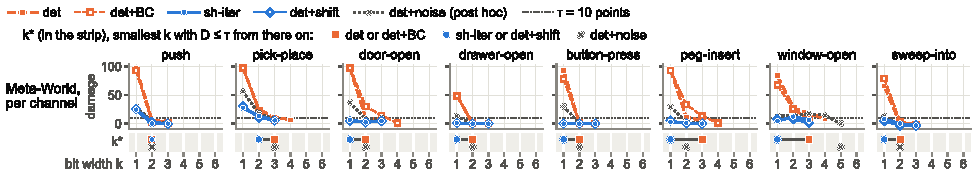
\includegraphics[width=\linewidth]{fig_bitlimit_pc.pdf}
\caption{Damage (success points) against bit width $k$ on Meta-World with per-channel ranges (E12; \detnoise post hoc), as in Figure~\ref{fig:bits}: the dotted line is $\tau=10$ points, missing markers: not run, and the strip under each panel marks the smaller $k^*$ of \dtm and \detbc (square), of \shiter and \detshift (circle) and of \detnoise (cross).}
\label{fig:bitspc}
\end{figure}

\textbf{Fresh noise on the bit axis (X5).} Table~\ref{tab:x5} sets $k^*$ of \detnoise next to the $k^*$ of E12. The E12 values come from another machine of the same type and are not paired with X5, so the comparison is descriptive. The damage of \detnoise is often not monotone in the bit width (per tensor, door-open loses \nv{x5.pt.dooropen3} points at 3 bits but \nv{x5.pt.dooropen2} at 2).

\begin{table}[h]
\caption{X5 (post hoc): smallest usable bit width of \detnoise on Meta-World next to E12's $k^*$ of \dtm / \detbc / \shiter / \detshift, and the bits that \detnoise gains over the better of \dtm and \detbc ($G_{\mathrm{noise}}$).}
\label{tab:x5}
\centering\small
\setlength{\tabcolsep}{4pt}
\begin{tabular}{@{}lcccccc@{}}
\toprule
 & \multicolumn{3}{c}{PT} & \multicolumn{3}{c}{PC} \\
\cmidrule(lr){2-4}\cmidrule(l){5-7}
Task & $k^*$ \detnoise & $k^*$ E12 & $G_{\mathrm{noise}}$ & $k^*$ \detnoise & $k^*$ E12 & $G_{\mathrm{noise}}$ \\
\midrule
\inputrows{tables/tabI_x5.tex}
\bottomrule
\end{tabular}
\end{table}

\textbf{The policy without planning (X6).} Table~\ref{tab:x6} compares TD-MPC2's policy, run without planning, with the unquantized planner on the 90 E11 pairs of each task, and sets it next to the lowest-bit dither configuration of E12 (the smallest $k^*$; among ties, the smaller damage at $k^*$, then per tensor before per channel and \shiter before \detshift). The policy uses the same FP32 encoder and $\pi$ as the planner and never calls the dynamics or reward networks, so it is not quantized; the comparison asks whether the low-bit planner falls below the policy. On Meta-World the policy comes close to the unquantized planner, and the dither configuration is better than the policy in \nv{x6.mw.better} task and the same in \nv{x6.mw.same}; on DMC the policy loses much more, and the dither configuration is better in \nv{x6.dmc.better} of the 4 tasks. Which configuration counts as lowest among ties changes some Meta-World comparisons, so we report these counts only here.

\begin{table}[h]
\caption{X6 (post hoc, D7): TD-MPC2 5M without planning (FP32 policy, mean action) against the unquantized planner (none), 90 pairs: success (\%) on Meta-World, return on DMC, and $D_{\mathrm{policy}}$ (points, \% of return on DMC); next to it the lowest-bit dither configuration of E12 (range, rounding, $k$) and its damage. Better/worse: the two intervals do not overlap; same: they overlap. The DMC cells of E12 have 45 pairs (two-stage cells, intervals not corrected for the interim look).}
\label{tab:x6}
\centering\scriptsize
\setlength{\tabcolsep}{3.5pt}
\begin{tabular}{@{}lrrllrrl@{}}
\toprule
 & & & & \multicolumn{3}{c}{Lowest dither configuration (E12)} & \\
\cmidrule(lr){5-7}
Task & none & policy & $D_{\mathrm{policy}}$ & configuration & $D$ & pairs & vs.\ policy \\
\midrule
\inputrows{tables/tabI_x6.tex}
\bottomrule
\end{tabular}
\end{table}
\clearpage


% PLAN 4.4 J: what did not hold, and claims we do not make. Source: FINAL_A 4.2-4.3, CLAIMS_tmlr 3, CLAIMS_rss 3.
\FloatBarrier
\section{What Did Not Hold}
\label{app:neg}
% Appendix J -- What Did Not Hold (body). Sources: main/reports/FINAL_A.md 4.2-4.3, rss_ext/CLAIMS_rss.md 3,
%   tmlr_ext/CLAIMS_tmlr.md 3; outcomes from Table tab:tests (keys b.*, e11.*, e17.*, dw.*, x17.*).
\textbf{Tests and predictions that did not hold.}
\begin{itemize}\setlength{\itemsep}{1pt}\setlength{\parskip}{0pt}
\item \emph{The OEI tests.} The original mechanism tests failed: \shiter's OEI was not near zero (H2a, \nv{b.h2a.n} of 4 mechanism tasks; push \nv{b.h2a.push.shiter}), also when the executed plan was re-scored with an independent draw (\nv{b.h2aindep.n} of 4), and the OEI did not rank the damage better than the one- and three-step errors (H2b: \nv{b.h2b.td} in TD-MPC2, \nv{b.h2b.dw} in DINO-WM, against a threshold of 0.15). The first failure is the winner's curse that the theory predicted (Appendix~\ref{app:theory}); after E1 the mechanism claim was narrowed to drift, tested on new seeds for TD-MPC2 and on the E1 cell for PushT (H2a$'$).
\item \emph{Near-tie density.} The benefit of sharing a draw did not grow with the density of near ties (H4b: Spearman \nv{b.h4b.rho}), although sharing helped in most tasks.
\item \emph{DMC.} The variant \shiter repaired \nv{e1.dmc.nfix} of \nv{e1.dmc.naff} damaged DMC cells in E1 (H3a fails for DMC) and was harmful on walker at 3 bits ($D_{\shiter}-D_{\dtm}$ \nv{b.h3a.walker}\% of return); in E11 it repaired \nv{e11.dmc.nfix.shiter} of \nv{e11.dmc.ndam}. With 12 iterations the better dither repairs \nv{e15.it1.n} of the 4 tasks (It1), but walker stays unrepaired even at 24 iterations ($\red$ \nv{e15.walker.red24}).
\item \emph{Better post-training quantizers.} On top of the best post-training quantizer, the extra gain of \shiter was borderline in TD-MPC2 (\nv{b.h3b.td} cells, exactly the threshold) and found in DINO-WM in only one of three cells (\nv{b.h3b.dw}), where the quantizer alone left little damage.
\item \emph{The PushT positive control.} Holding the full-size shared dither fixed for the plan (\shplan) should have brought back \dtm's drift on PushT, as it did in TD-MPC2; its drift ratio was \nv{e2.drift.pusht.shplan}. Only coarse tables were exploited in DINO-WM (Appendix~\ref{app:mech}). H2c also failed on PushT (Spearman of $N$ and damage \nv{b.h2c.pusht.d}), and the E3 expectation that tables kept per candidate behave like redrawn per-candidate dither failed in \nv{e.e3.indstep.n}--\nv{e.e3.indep.n} of 12 TD-MPC2 tasks.
\item \emph{Wall in E1.} None of the planned Wall cells was damaged, and at 4 bits \dtm beat the unquantized model, so Wall contributed only an exploratory cell to E1.
\item \emph{Fresh noise (B3).} We predicted that adding fresh noise to \dtm would not repair a majority of the damaged cells in any benchmark; it repaired \nv{e11.mw.nfix.detnoise} of \nv{e11.mw.ndam} Meta-World cells, though only \nv{e11.dmc.nfix.detnoise} of \nv{e11.dmc.ndam} DMC cells and neither damaged DINO-WM cell, and on the bit axis it held up less well than dither (Section~\ref{sec:noise}).
\item \emph{Dg1 on DINO-WM.} The summary statistic did not beat the latent one-step error by the planned margin on DINO-WM's single damaged cell (\nv{dg1.dw}).
\item \emph{PushT at 4 bits on the new split.} The E1 damage (\nv{e1.pusht4.D.det} points) did not reappear on the new split (\nv{dw.pusht4.D.det}); re-running the E1 pairs on the new GPU type reproduced it (\nv{x17.D.det}), so the split, not the hardware, explains the difference (post hoc, X17).
\item \emph{Latency and formats.} The kernel overhead of \detshift exceeded 5\% at $N=512$ (K1 held in only \nv{e17.k1.n} of \nv{e17.k1.of} conditions; \nv{e17.detshift.5m512}\% and \nv{e17.detshift.317m512}\%). Pre-converted BF16 was not lossless (K3: \nv{e17.k3.n} of \nv{e17.k3.of} tasks without damage; door-open \nv{e17.bf16.dooropen} points, cheetah-run \nv{e17.bf16.cheetah}\%). The integer rollout was not faster than pre-converted BF16 (L2c: \nv{b.l2c.range}$\times$ its time), nor was the whole planning step (S2: \nv{b.s2.range}$\times$). In eager execution the integer kernel was slower than FP32 (E7), and H5's cases where dither with fewer bits Pareto-dominates \dtm with more were weak (push only). NVFP4 caused too little damage for F1 (\nv{b.f1.nv} of 12 tasks), and on DMC the FP4 cells were not repaired (F2: \nv{b.f2.dmc}).
\item \emph{Few iterations and weights.} With one MPPI iteration \shiter is no better than \dtm, and in the E7 kernel at three iterations dither was harmful on DMC. Stochastic rounding of weights helped in TD-MPC2 and hurt in DINO-WM.
\end{itemize}

\textbf{Claims we do not make.}
\begin{itemize}\setlength{\itemsep}{1pt}\setlength{\parskip}{0pt}
\item That the OEI predicts damage better than one-step error, or that planners do not exploit redrawn noise: the winner's curse of the last selection arises under fresh noise too.
\item That one-step or multi-step error is the wrong measure in general. Our statement concerns the variants at one bit width; across bit widths the one-step error ranks the damage, errors over several steps separate \dtm in DINO-WM, and the reward error partly separates it in TD-MPC2.
\item That persistence decides the outcome in both families, that DINO-WM is dominated by mean bias (\detbc is worse than \dtm on PushT), or that the model family causes which component dominates: E16 swapped only the planners' update rules, and the families differ in more than the planner.
\item That any noise or that randomization alone removes the damage, or that a low persistent share implies repair: \detnoise repairs Meta-World but not DMC or DINO-WM.
\item That a loss of resolution causes \dtm's damage in TD-MPC2: fixed random thresholds repair at most \nv{e11.mw.nfix.shep} of \nv{e11.mw.ndam} Meta-World cells.
\item That bias correction is a remedy, that \shiter alone gains a bit in most Meta-World tasks (it does so in \nv{e12.pt.nG.shiter} per tensor and \nv{e12.pc.nG.shiter} per channel, of \nv{e12.mw.n}), or that dither gains two bits on Wall (\nv{dw.wall.G.range}).
\item That $\rho_p\cdot\sigma_e/\sigma_J$, measured before deployment, predicts the damage: it nearly restates the manipulated variable and fails on DINO-WM.
\item That \detshift comes without latency cost, that pre-converted BF16 is lossless, that our integer W8A4 world model is faster than BF16, that 4-bit activations run faster than 8-bit ones on the GPUs we used, that low-bit arithmetic speeds up the whole planning step as much as the rollouts, or that the world model dominates the cost of a planning step.
\item That the fix works on DMC at the default number of iterations, with a single planner iteration, or in every task and planner setting.
\item That dither helps in general on top of strong post-training quantization, or any conclusion about quantization-aware training, whose baseline was weak.
\item That accelerator FP4 formats reproduce the failure of uniform grids, or that larger models are more robust to rounding: the primary bit widths at 317M are close to those at 5M.
\item That every persistent error is exploited, that a fixed dither obeys a $1/N_{\mathrm{eff}}$ law, or that sharing and redrawing are both always needed: in DINO-WM the full-size fixed table was not exploited.
\item That the PushT damage at 4 bits replicates on the new split.
\end{itemize}


% PLAN 4.4 K: compute and reproducibility. The repository URL appears only in the arXiv build (\ifarxiv);
%   the submission points to the anonymous supplement (PLAN 5.3).
\FloatBarrier
\section{Compute and Reproducibility}
\label{app:repro}
\ifarxiv
Code, design documents, run logs and result files are available at \url{https://github.com/thddydgnl/dithered-world-models}.
\else
Code, design documents, run logs and result files are provided as anonymized supplementary material.
\fi

% Appendix K -- Compute and Reproducibility (body after the \ifarxiv ... \fi sentence, which stays in main.tex).
% Sources: main/reports/FINAL_A.md 8.2-8.4, main/LOG.md, rss_ext/LOG.md, tmlr_ext/LOG.md and RESULTS_tmlr.md 4 (keys k.*,
%   kind 'report'); DESIGN_tmlr.md 0.2. Anonymous: no names, server, repository or home paths (PLAN 4.2 item 6, 5.3).
\textbf{Compute.} The main study (E0--E7) ran on two RTX A5000 GPUs of a local server and occupied them for about \nv{k.gpuh.main} GPU-hours: \nv{k.gpuh.td} hours of one GPU shared by 16 MPS processes for TD-MPC2 and \nv{k.gpuh.dw} GPU-hours for DINO-WM, including time slowed by sharing. The theory simulations took \nv{k.cpuh.e4} CPU-hours. The extension E8--E10 with E8c ran on rented A40, RTX 4090 and RTX 5090 GPUs for \$\nv{k.cost.rss}, and E11--E17 with the post hoc runs on rented A40 and RTX 4090 GPUs for \$\nv{k.cost.tmlr} (\$\nv{k.cost.tmlr.main} for the planned runs and \$\nv{k.cost.tmlr.posthoc} for D4--D6), including setup and idle time; X6 (D7) cost a further \$\nv{k.cost.x6}. Every job of E11--E17 completed; jobs hit by run incidents were re-run (Appendix~\ref{app:plan}).

\textbf{What the supplementary material contains.} The code of every stage as it ran; the design documents of all versions, two documents of them redacted (the main design and the initial experiment plan; Appendix~\ref{app:plan}); the coordinator and worker logs; the stage reports; and the result files the scripts read and the per-stage analysis outputs, including episode-level tables for the TD-MPC2 stages E9--E17. The raw job records of the cloud machines (about 210 MB) are not included. It is organized as the main study (designs, code, results per stage, reports), the extension E8--E10, and E11--E17 with one folder per group of runs (TD-MPC2 5M, 317M, DINO-WM, integer kernel), each holding its operational plan fixed before the main run, its code, results, log and report; a separate folder holds the scripts that recomputed the verdicts and the re-analyses R1--R5. Checkpoints and datasets are not included: they are the public releases of TD-MPC2 and DINO-WM, and their hashes are recorded. Upstream commits and software versions are listed in Appendix~\ref{app:details}.

\textbf{Recomputing every number.} Every result number in this paper is a macro defined in \texttt{numbers.tex}, which \texttt{build/make\_numbers.py} writes from the result files; each definition records the file and field it comes from. \texttt{build/make\_tables.py} writes every numeric table from the same files. \texttt{build/verify\_numbers.py} re-runs the computation and checks that \texttt{numbers.tex} is current, that every macro used in the text is defined, that statements whose wording depends on the data (``in all cells'', ``none harmful'', ``indistinguishable from zero'') agree with it, and that every number still typed in the text is a registered design constant or label. A few values exist only in the stage reports and logs (the compute and cost figures above and the number of simulated planner runs); \texttt{numbers.tex} marks them, and \texttt{verify\_numbers.py} lists them as not verified against data. Run from \texttt{paper/tmlr}, the commands \texttt{python3 build/make\_numbers.py}, \texttt{python3 build/make\_tables.py} and \texttt{python3 build/verify\_numbers.py --strict} regenerate and check all numbers from the supplementary material alone, without a GPU; these scripts use only the Python standard library (with a UTF-8 locale), and the figures additionally need matplotlib and PyMuPDF. The supplement includes an anonymized copy of the manuscript source, which \texttt{verify\_numbers.py} reads, and a README that maps every table and figure to its result files. The episode-level tables of E9--E17 on TD-MPC2 allow their intervals to be recomputed (paired bootstrap, $10^4$ resamples, NumPy \texttt{RandomState(0)}); for E1--E7 and for DINO-WM the supplement holds the per-cell and per-job summaries, whose episode records are part of the raw job records. The verdicts of E11, E14, K2 and the DINO-WM stages were recomputed from the raw job records by scripts independent of the analysis code. These scripts and their outputs are included, but the raw records they read are not.

\textbf{Re-running the experiments.} Seeds are listed in Appendix~\ref{app:details}. Results are bit-identical only on the same GPU type and software stack: on a second machine of the same type, the E11 cells of \detnoise and of the unquantized model were reproduced bit for bit, the first jobs of every new DINO-WM machine matched those of the first one bit for bit, and on another GPU type the planner outputs differ while the episode outcomes agree in most episodes (X17, Appendix~\ref{app:new}).


\end{document}
